This appendix presents more details on the measurement of the data-driven real lepton efficiency using the $Z$ tag-and-probe method.

%%%
%%%
%%%

\section{The $Z$ tag-and-probe method}
\label{sec:app_RLE_ZTandP_method}
The $Z$ tag-and-probe method is used to extract the leptons from data and measure the real lepton efficiency.
The selected events are required to have at least two baseline leptons.
The lepton candidates with $\pt > 25$~{\GeV} and satisfying all the signal lepton requirements are categorized into \textit{tag leptons}.
The lepton candidates passing baseline lepton requirements can be classified as \textit{probe leptons}.
In order to form a tag-and-probe pair, the two selected leptons have to carry the same flavor and opposite charge.
The invariant mass of the tag-and-probe pair system should satisfy the $Z$ boson mass window $80 < m_{\ell \ell} < 100$~{\GeV}.
All possible combinations of the tag-and-probe pairs are considered to avoid any bias and to increase the statistics.
For the $Z \to ee$ decay, an additional $|\eta| < 2$ requirement is applied on the tag and probe leptons.
However, no additional requirement is applied for the $Z \to \mu \mu$ decay.
The tag lepton is used to select the probe lepton only and the probe lepton is used for the real efficiency measurements.
In this study, the tag and probe leptons are required to match the lepton triggers listed in Table~\ref{tab:app_RLE_single_lepton_triggers}.

\begin{table}[htb]
    %\begin{center}
    \resizebox{\textwidth}{!}{% <------ Don't forget this %
        \begin{tabular}{cccc}
            \hline
            \hline
            Trigger                                & lepton   & 2015                                     & 2016\\
            \hline
            \multirow{2}{*}{Single lepton trigger} & electron & \texttt{e24\_lhmedium\_iloose\_L1EM20VH} & \texttt{e26\_lhtight\_nod0\_ivarloose}\\
                                                   & muon     & \texttt{mu20\_iloose\_L1MU15}            & \texttt{mu26\_ivarmedium}\\
            \hline
            \multirow{2}{*}{Dilepton trigger}      & electron & \texttt{2e12\_lhloose\_L12EM10VH}        & \texttt{2e17\_lhvloose\_nod0}\\
                                                   & muon     & \texttt{mu18\_mu8noL1}                   & \texttt{mu22\_mu8noL1}\\
            \hline
            \hline
        \end{tabular}
    }
    %\end{center}
    \caption{The list of single lepton and dilepton triggers used for the real lepton efficiency measurements.
    The dilepton triggers are used for studying the systematic uncertainties causing by the trigger.}
    \label{tab:app_RLE_single_lepton_triggers}
\end{table}

Figure~\ref{fig:app_RLE_mll_distributions} shows the data-to-MC comparison of the tag-and-probe pair invariant mass distributions which indicate the need of subtracting the background especially for the probe electron with $\pt < 20$~{\GeV}.
%
\begin{figure}[htb]
    \begin{center}
        \begin{subfigure}[b]{0.48\textwidth}
            \begin{center}
                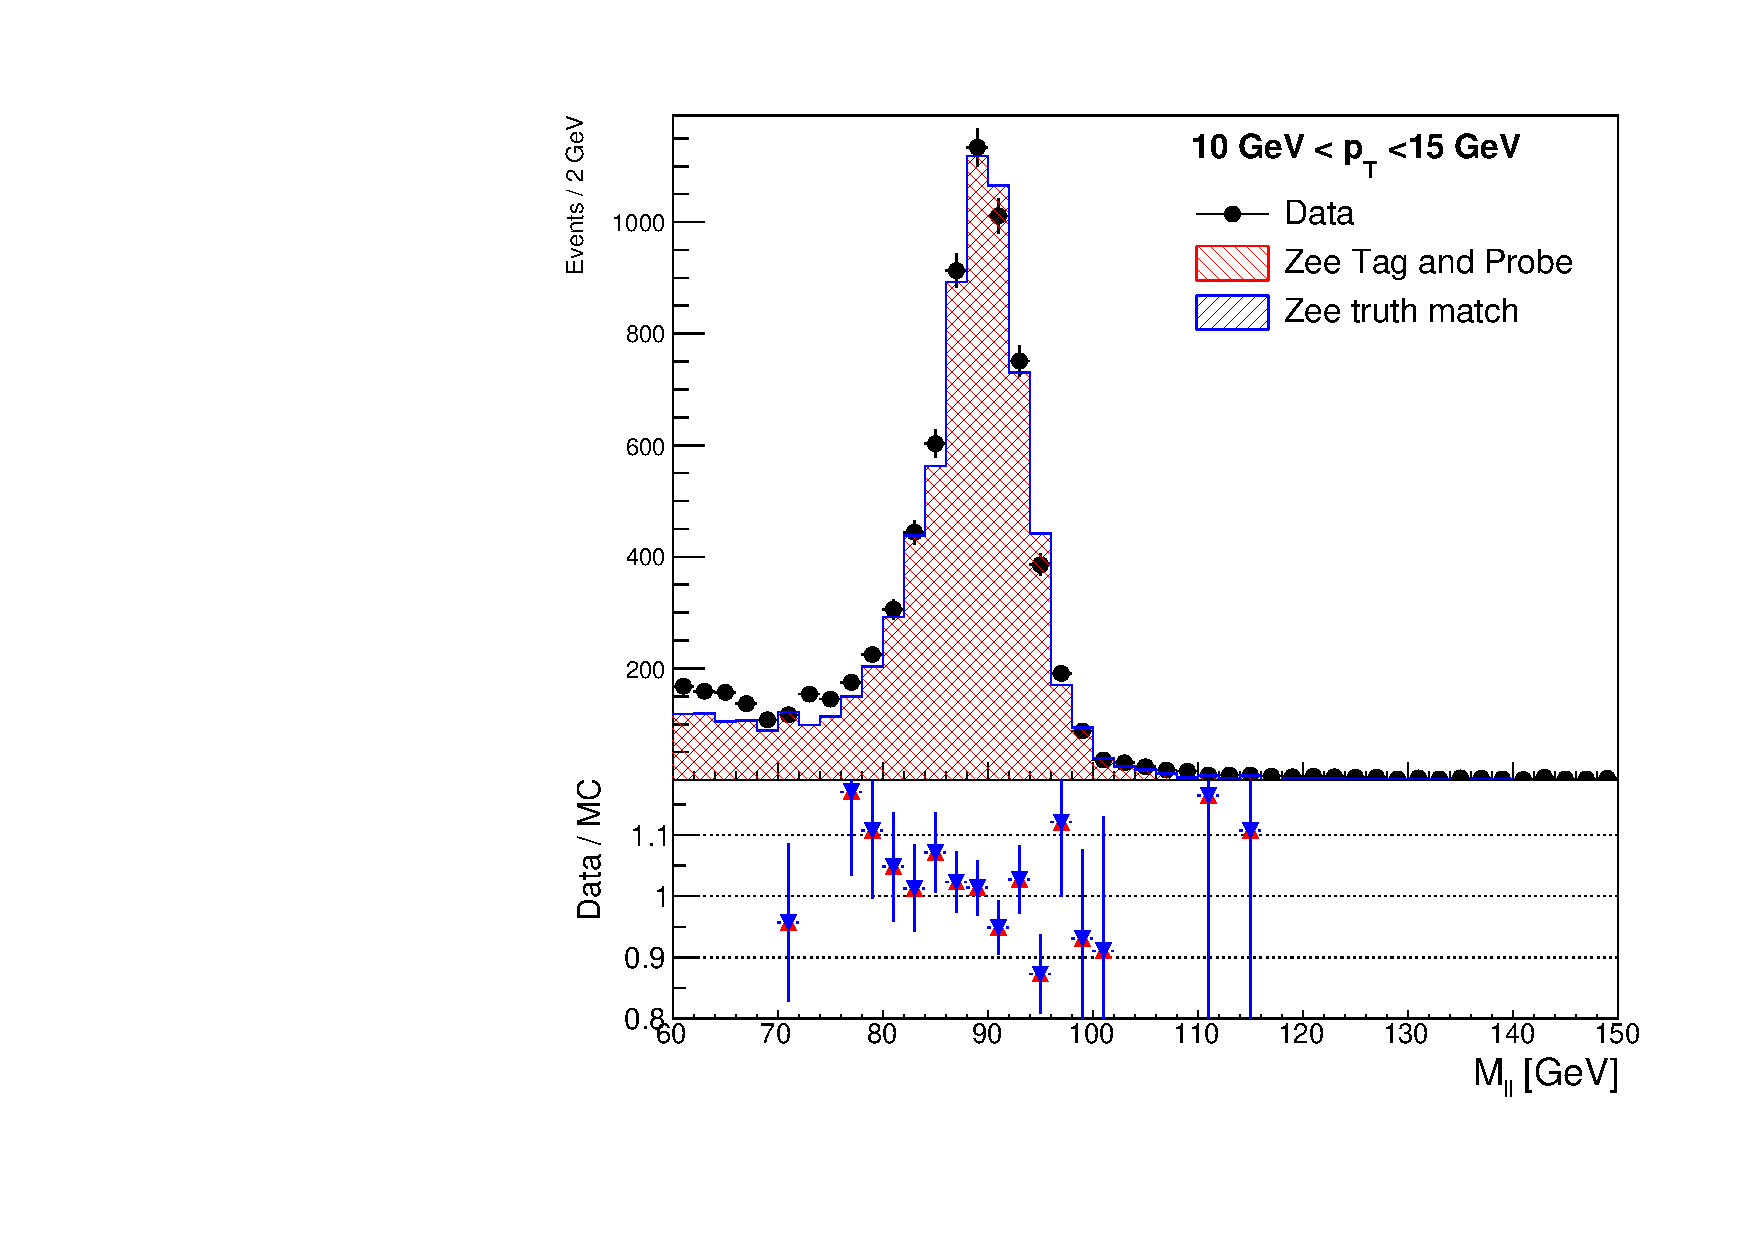
\includegraphics[scale=0.4]{signal_level_Mee_pt1015_ratio_plot_MC_normalized.pdf}
                \caption{The $m_{ee}$ distribution with $10 < \pt < 15$~{\GeV}.}
            \end{center}
        \end{subfigure}%
        \begin{subfigure}[b]{0.48\textwidth}
            \begin{center}
                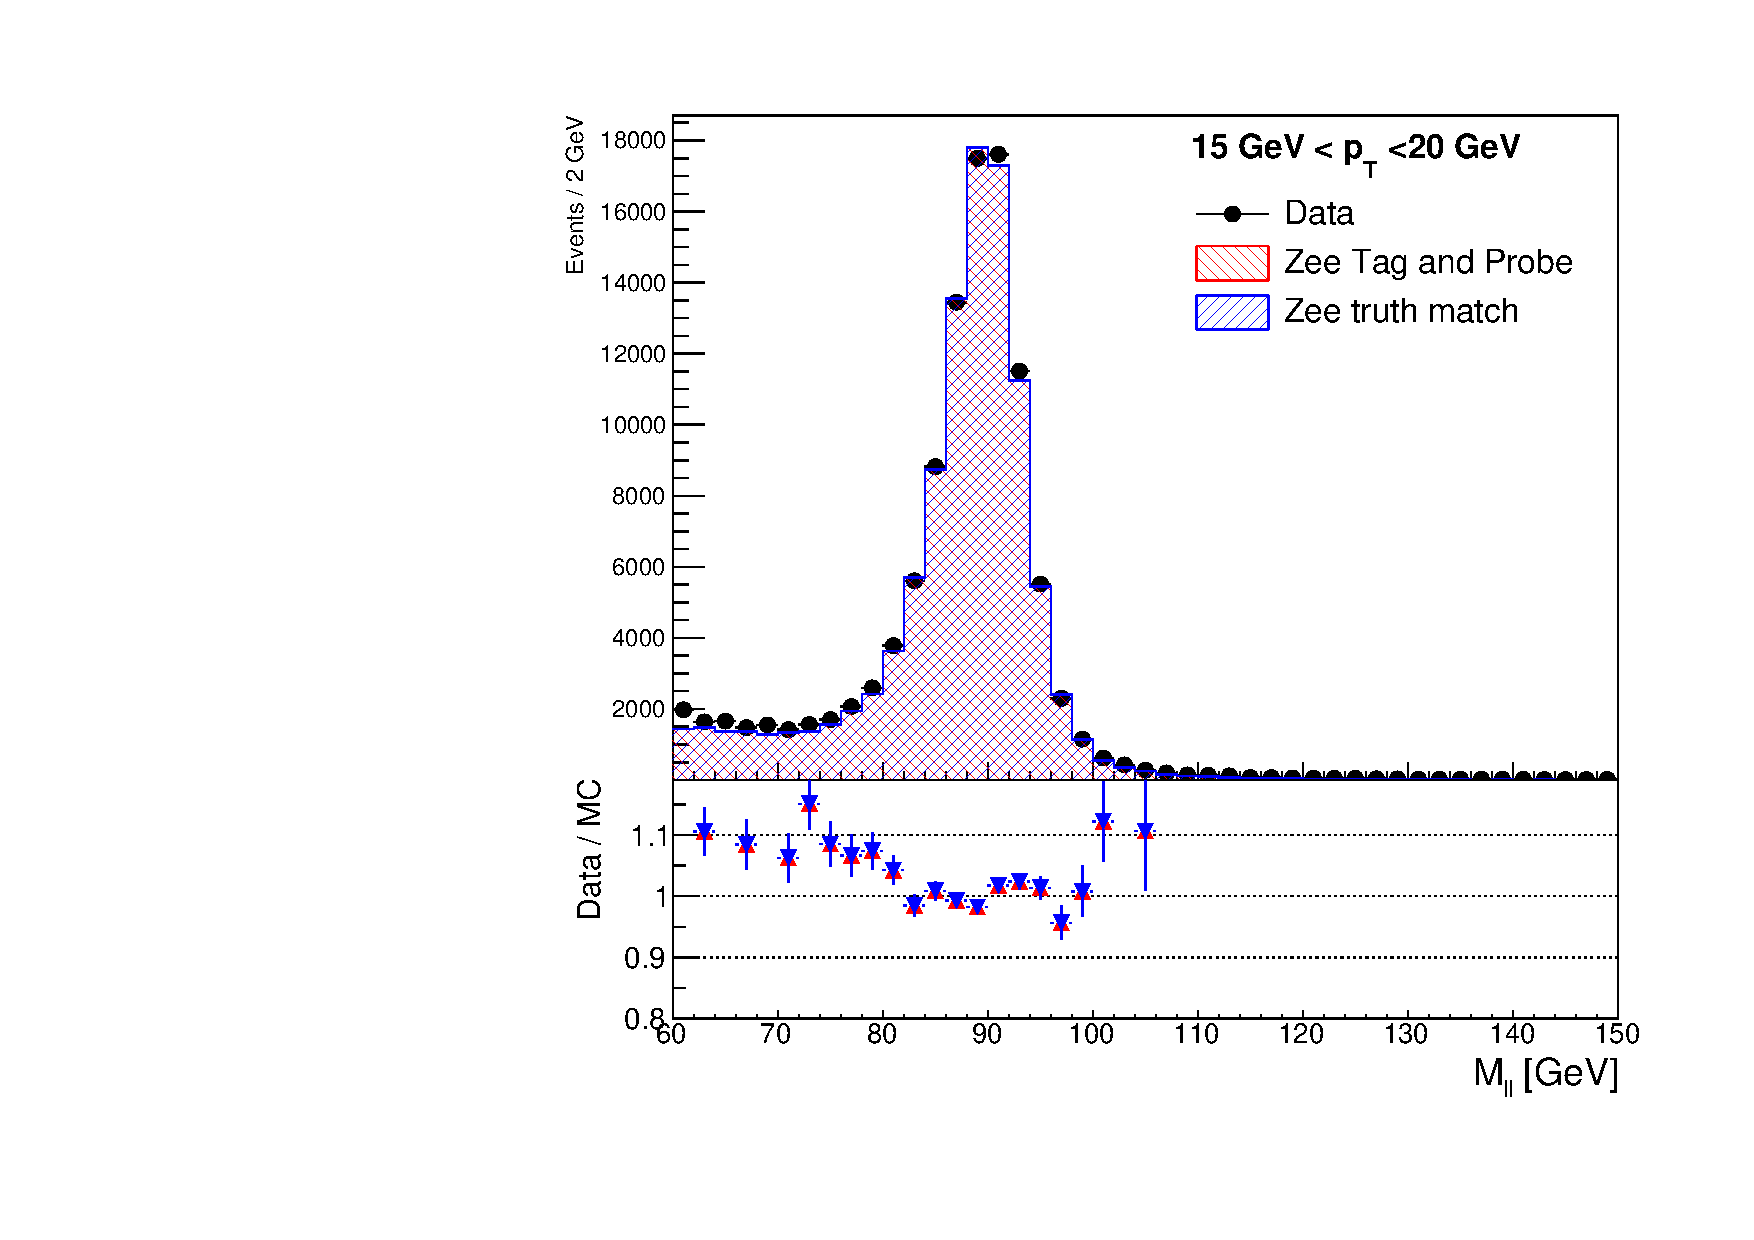
\includegraphics[scale=0.4]{signal_level_Mee_pt1520_ratio_plot_MC_normalized.pdf}
                \caption{The $m_{ee}$ distribution with $15 < \pt < 20$~{\GeV}.}
            \end{center}
        \end{subfigure}
        \begin{subfigure}[b]{0.48\textwidth}
            \begin{center}
                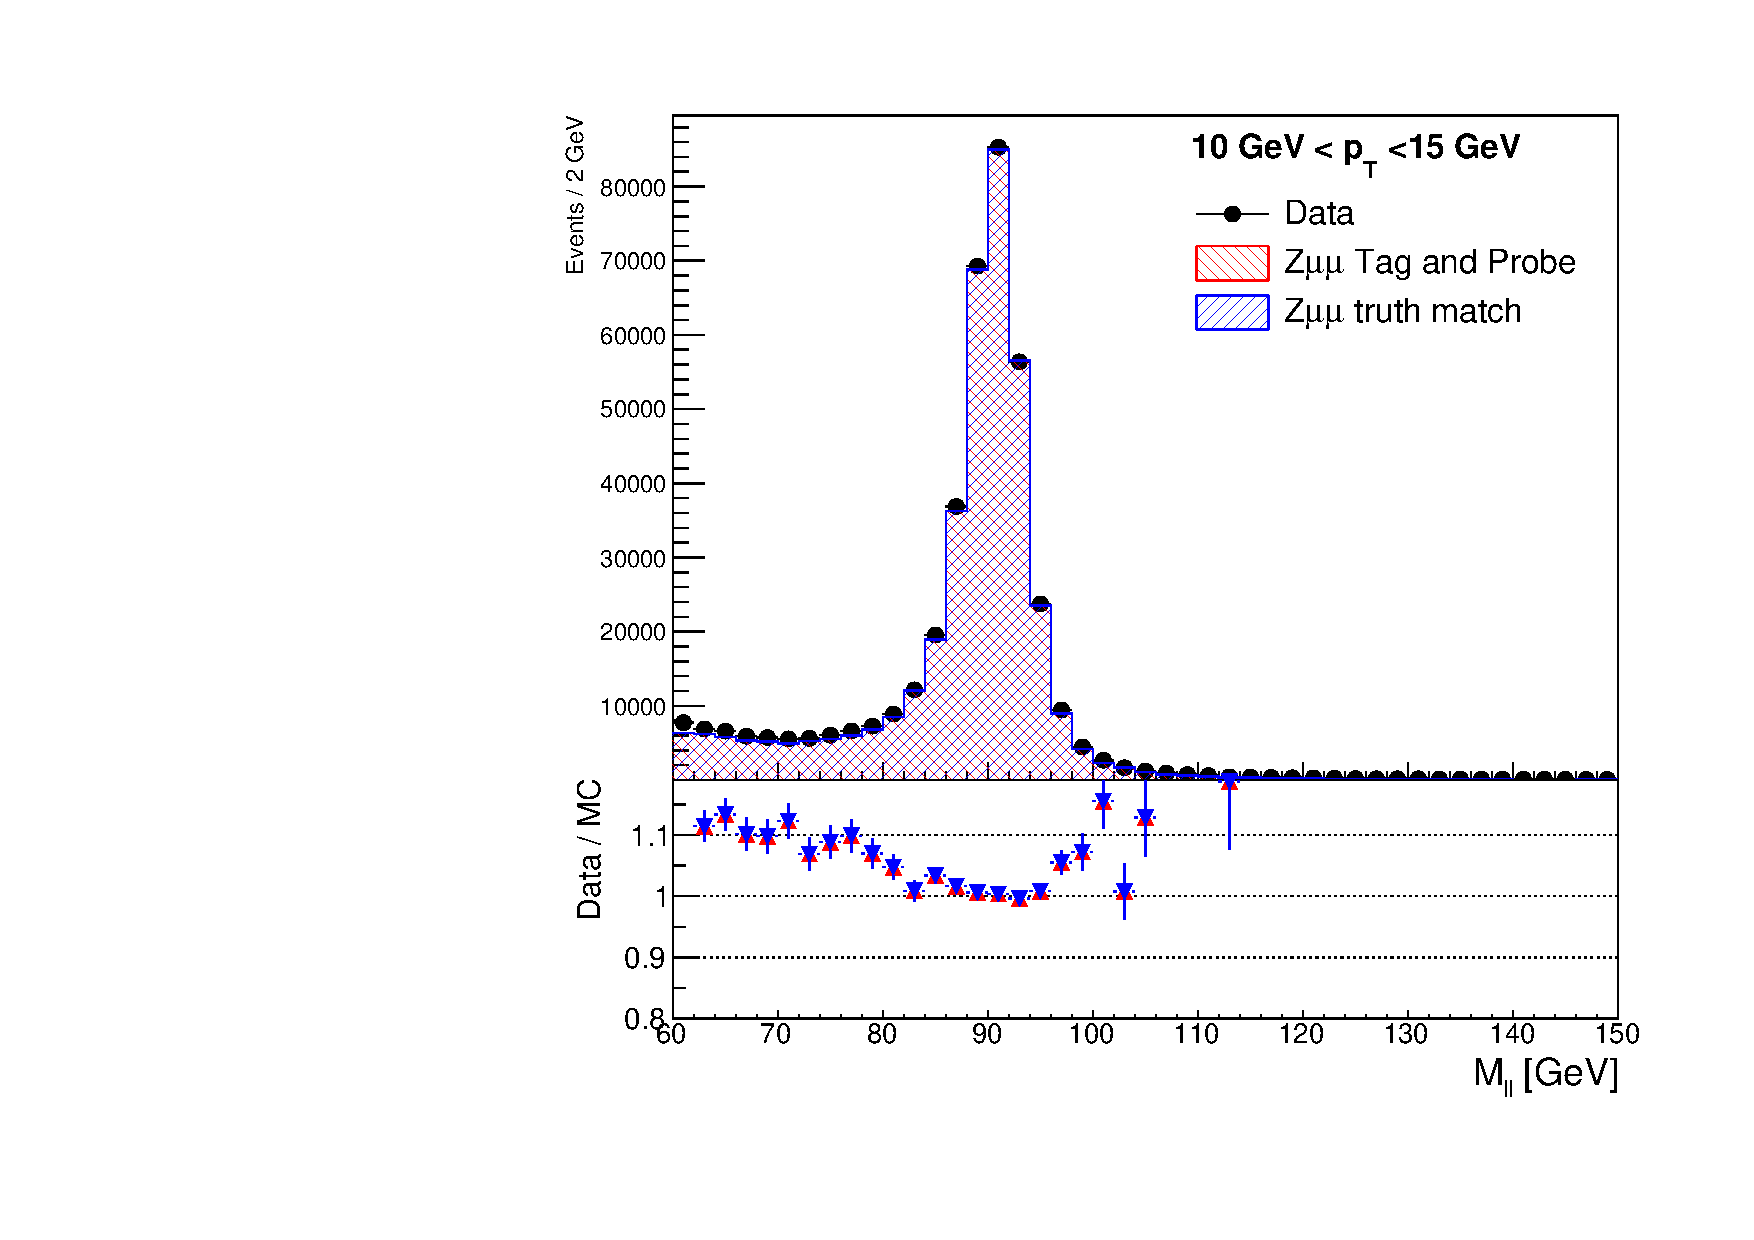
\includegraphics[scale=0.4]{signal_level_Mmumu_pt1015_ratio_plot_MC_normalized.pdf}
                \caption{The $m_{\mu\mu}$ distribution with $10 < \pt < 15$~{\GeV}.}
            \end{center}
        \end{subfigure}%
        \begin{subfigure}[b]{0.48\textwidth}
            \begin{center}
                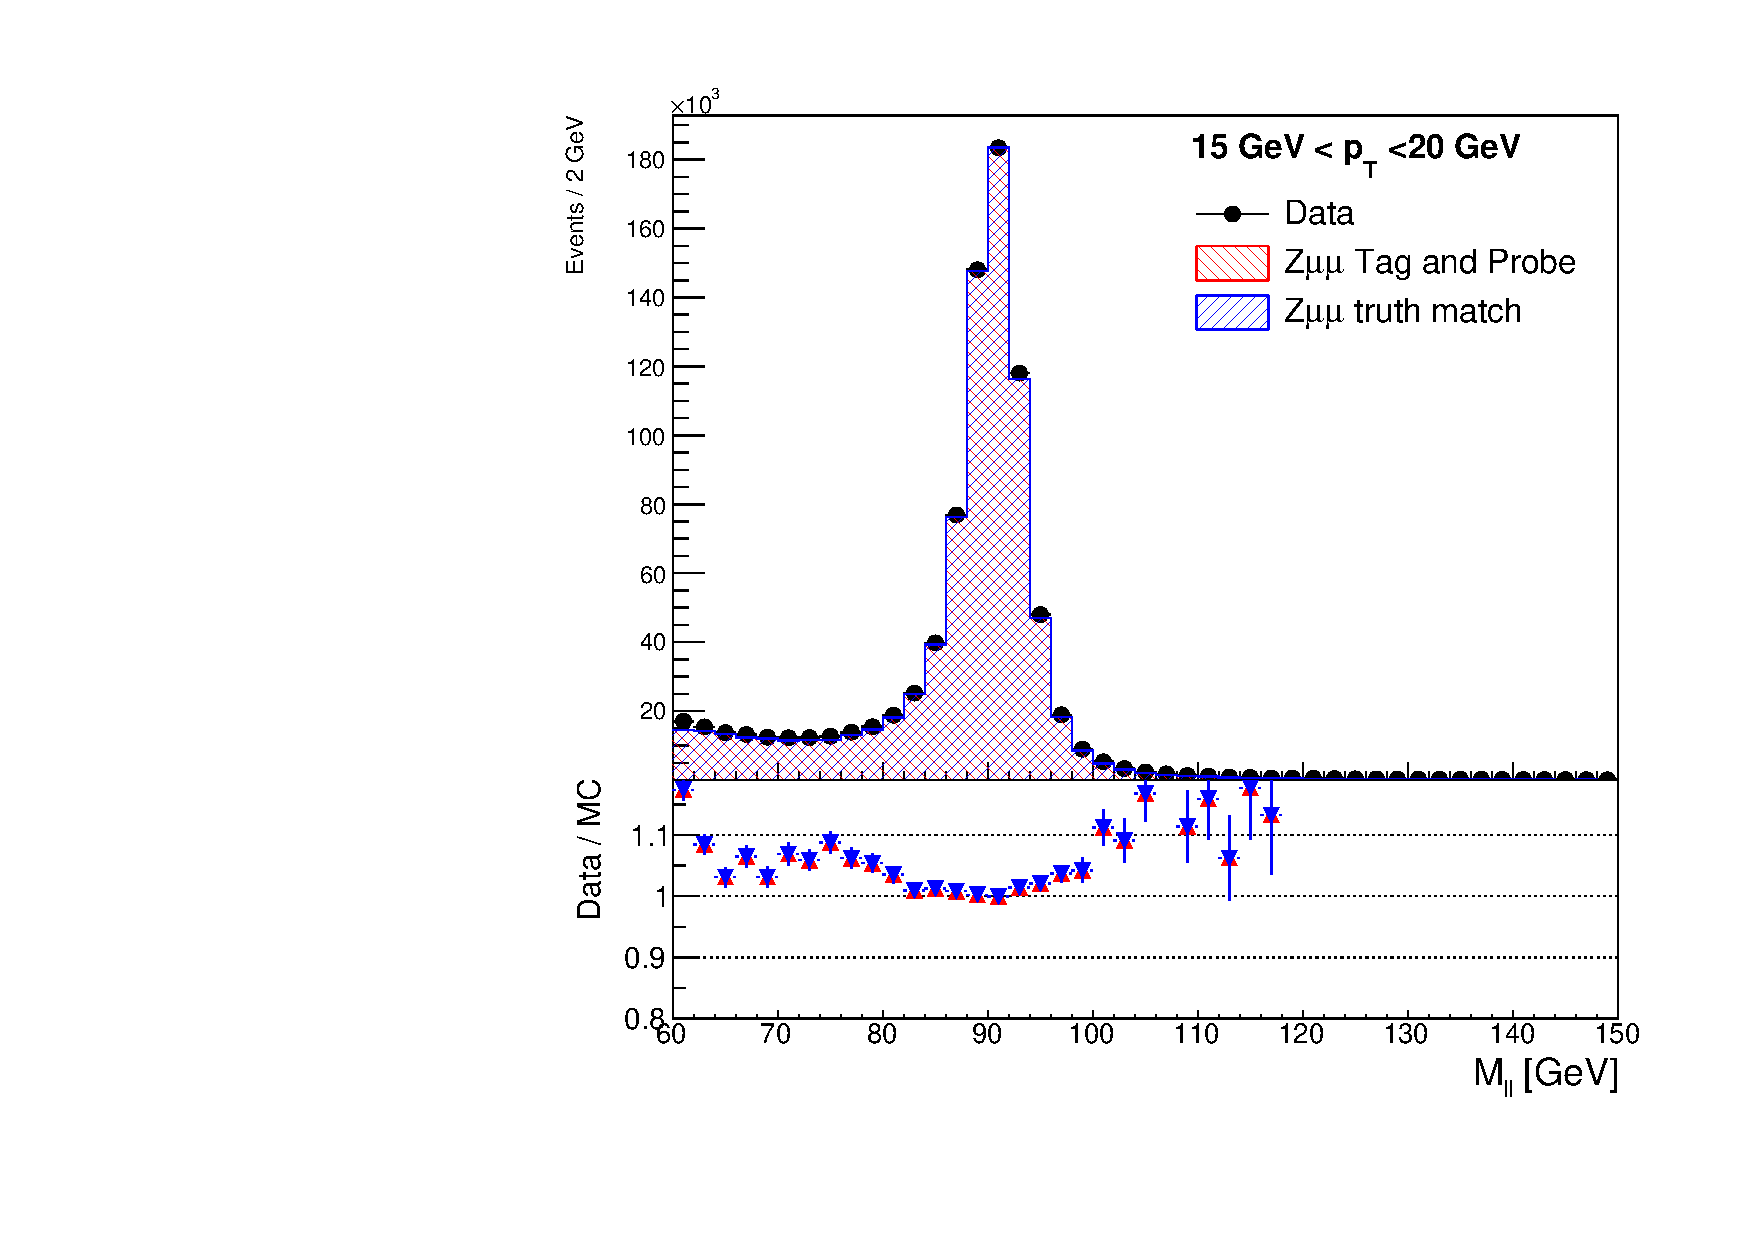
\includegraphics[scale=0.4]{signal_level_Mmumu_pt1520_ratio_plot_MC_normalized.pdf}
                \caption{The $m_{\mu\mu}$ distribution with $15 < \pt < 20$~{\GeV}.}
            \end{center}
        \end{subfigure}
    \end{center}
    \caption{The invariant mass distributions of the tag-and-probe pair computed using $Z+jets$ MC and 2015 + 2016 data.
    The red color stands for the $Z$ tag-and-probe events, the blue color represents the $Z$ truth matched events, and the black dots are data.
    The MC distributions are scaled to the data using a Gaussian fit of the $Z$ mass peak $85 < m_{\ell \ell} < 95$~{\GeV}.}
    \label{fig:app_RLE_mll_distributions}
\end{figure}
%
A background template method, which is similar to the one used by the $e/\gamma$ performance group for their efficiency measurements~\cite{ATLAS-CONF-2014-018}, is used to estimate the background contamination from the low \pt electrons.
No background subtraction is performed on the signal leptons because the background contamination is found to be negligible.
However, the background contamination in the baseline probe leptons needs to be subtracted.
The real lepton efficiency is obtained by the following equation
%
\begin{equation}
    \epsilon = \frac{N_{\mathrm{signal}}}{N_{\mathrm{baseline}} - N_{\mathrm{baseline}}^{bkg}}
    \label{eq:app_RLE_efficiency_formula}
\end{equation}
%
where $N_\mathrm{signal}$ is the number of probe leptons passing the signal requirements, $N_\mathrm{baseline}$ is the number of probe leptons passing the baseline requirements, and $N_\mathrm{baseline}^{bkg}$ is the estimated background contamination in the baseline probe leptons.

%%%
%%%
%%%

\section{Background subtraction}
\label{sec:app_RLE_bkg_subtraction}
The background template method is used to evaluate the background contamination on data.
By inverting the calorimeter and track isolations, requesting the electron object to fail the medium LH identification, the background sample enriched template can be obtained.
Three background templates are considered for the systematic study.
The definitions of the background template are summarized in Table~\ref{tab:app_RLE_bkg_templates}.
%
\begin{table}[htb]
    %\begin{center}
    \resizebox{\textwidth}{!}{% <------ Don't forget this %
        \begin{tabular}{cccc}
            \hline
            \hline
            cut                   & variation 1 template                   & baseline template                       & variation 2 template\\
            \hline
            Identification        & -                                      & fail medium LH                          & fail medium LH\\
            Calorimeter isolation & $E_\mathrm{T}^{topocone20} /\pt > 6\%$ & $E_\mathrm{T}^{topocone20} /\pt > 15\%$ & $E_\mathrm{T}^{topocone20} /\pt > 20\%$\\
            Track isolation       & $p_\mathrm{T}^{varcone20} /\pt > 6\%$  & $E_\mathrm{T}^{topocone20} /\pt > 8\%$  & $E_\mathrm{T}^{topocone20} /\pt > 15\%$\\
            \hline
            \hline
        \end{tabular}
    }
    %\end{center}
    \caption{The definition of the background templates for estimating the background contamination associated with the $Z$ tag-and-probe method.
    The baseline template is used to estimate the background contamination.
    The variation 1 template has looser requirements and the variation 2 template has tighter requirements.
    They are used to assess the systematic caused by the background contamination.}
    \label{tab:app_RLE_bkg_templates}
\end{table}
%
Figure~\ref{fig:app_RLE_bkg_templates} shows the $m_{ee}$ distributions of the background template.
%
\begin{figure}[htb]
    \begin{subfigure}[b]{0.48\textwidth}
        \begin{center}
            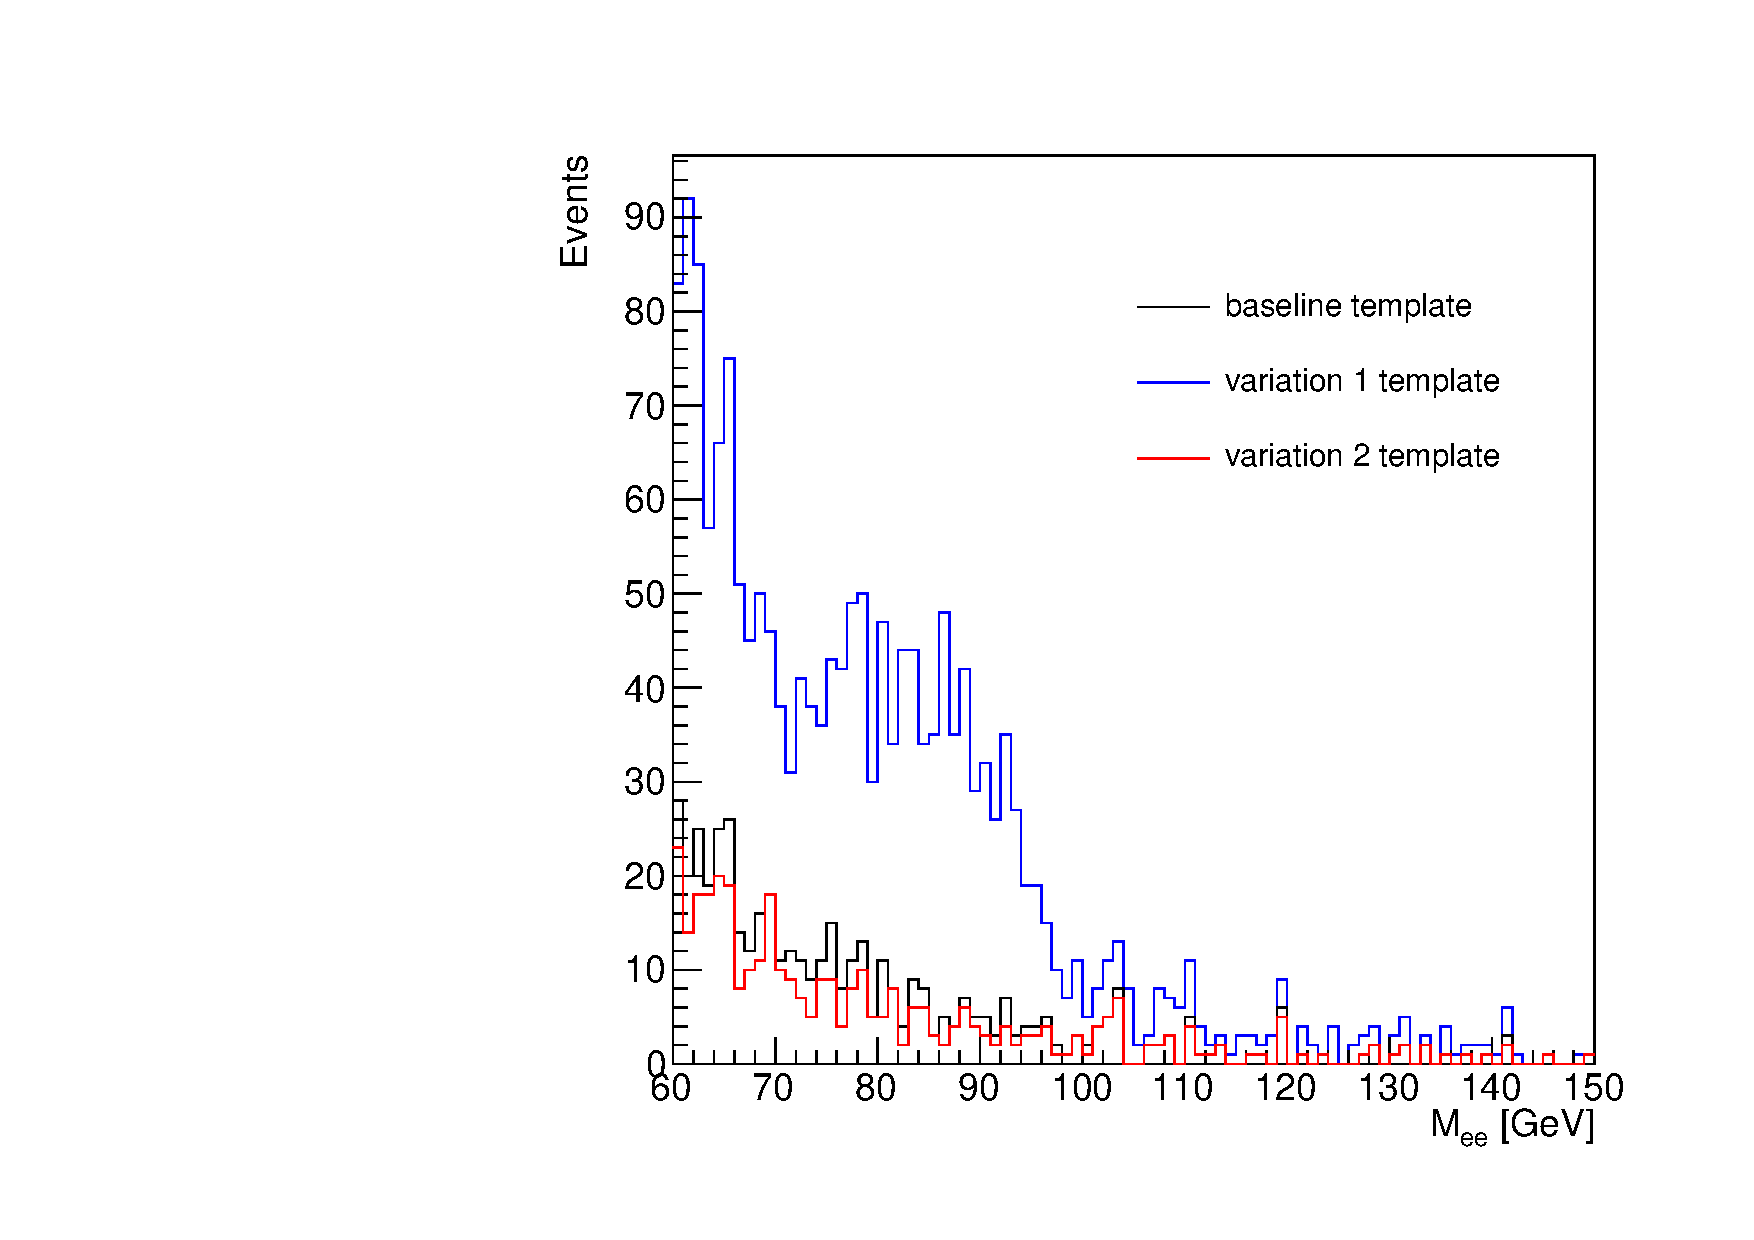
\includegraphics[scale=0.4]{bkg_template_electron_pt_1015_eta0201.pdf}
            \caption{Probe electrons with $10 < \pt < 15$~{\GeV}.}
        \end{center}
    \end{subfigure}
    \begin{subfigure}[b]{0.48\textwidth}
        \begin{center}
            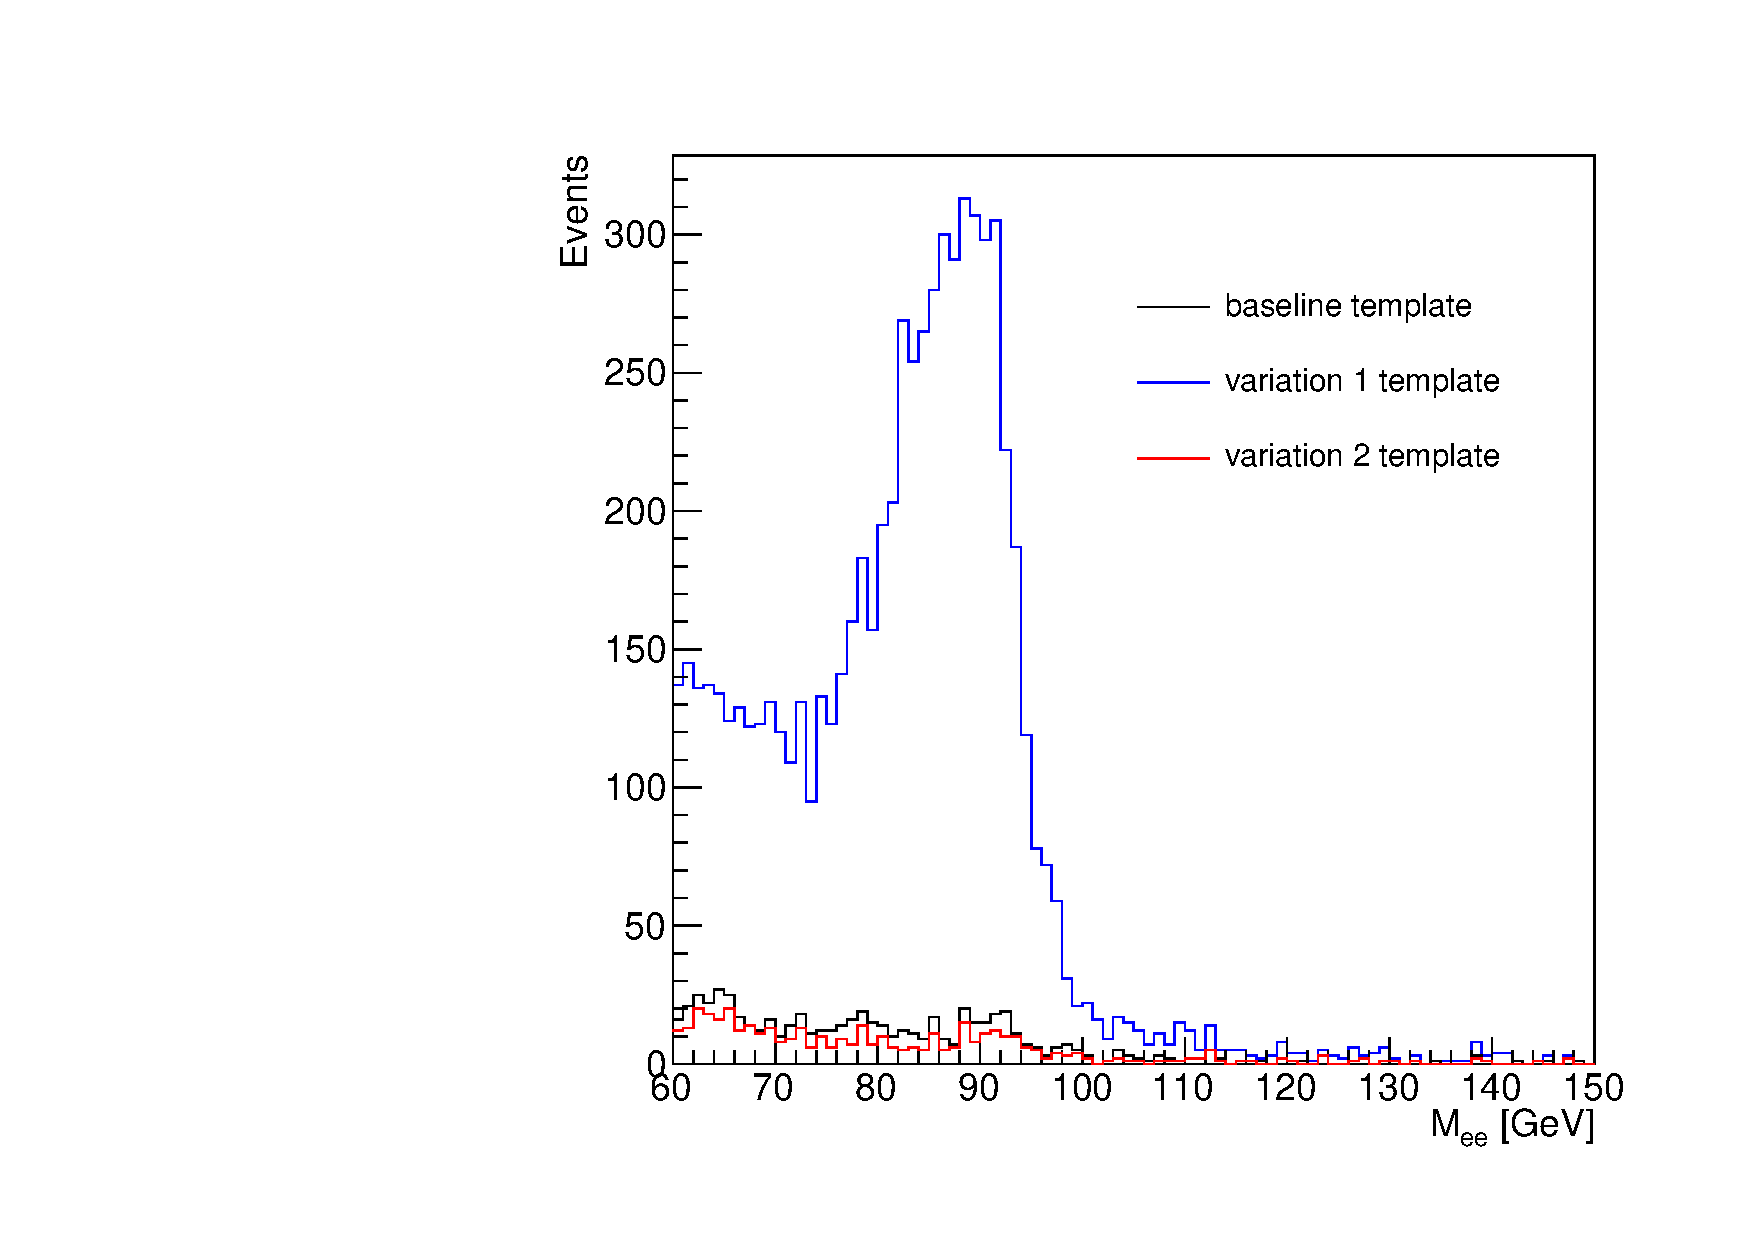
\includegraphics[scale=0.4]{bkg_template_electron_pt_1520_eta0201.pdf}
            \caption{Probe electrons with $15 < \pt < 20$~{\GeV}.}
        \end{center}
    \end{subfigure}
    \caption{The $m_{ee}$ distributions for the baseline, variation 1 and variation 2 background templates.
    The $m_{ee}$ distributions are computed using the probe electrons with different \pt as indicated in the caption of plots.
    The variation 1 template has looser calorimeter and track isolation requirements and the baseline and the variation 2 templates have tighter selection criteria.
    So a peak can be seen in the $Z$ mass region in variation 1 template but not in the baseline and variation 2 templates.}
    \label{fig:app_RLE_bkg_templates}
\end{figure}
%
The invariant mass distribution of the template events ($m_{ee}^\mathrm{template}$) is then used to estimate the amount of background in $80 < m_{\ell \ell} < 100$~{\GeV} region.
In order to estimate the correct of background events, the $120 < m_{ee} < 150$~{\GeV} region is used to normalize the background template because a smaller prompt electron contribution is expected in this region.
Equation~\ref{eq:app_RLE_bkg_in_the_tail} shows the estimation of the number of background events in the tail region using the baseline electrons.
%
\begin{equation}
    N_{bkg}^\mathrm{tail} = N_\mathrm{baseline}^\mathrm{tail} - N_\mathrm{MC, prompt}^\mathrm{tail}
    \label{eq:app_RLE_bkg_in_the_tail}
\end{equation}
%
where $N_\mathrm{baseline}^\mathrm{tail}$ can be obtained by integrating the baseline $m_{ee}$ distribution in the tail region and $N_\mathrm{MC, prompt}^\mathrm{tail}$ is the prompt electron contamination which is estimated by integrating the $m_{ee}$ distribution in the tail region using the $Z \to ee$ MC simulation.
Because the baseline electron selection criteria already provides a relatively high purity of prompt electrons, the background template suffers from low statistics in the tail region.
The template is fitted in region $60 < m_{ee}^\mathrm{template} < 120$~{\GeV} using an exponential function to avoid any bias in the normalization factor due to statistical fluctuations.
However, the $80 < m_{ee}^\mathrm{template} < 100$~{\GeV} is excluded to minimize the prompt lepton contamination arising from $Z \to ee$ decays.
The fit is mostly driven by the $60 < m_{ee}^\mathrm{template} < 80$~{\GeV} due to the low statistics in the tail.
After fitting is performed, the template in the tail region $N_\mathrm{template}^\mathrm{tail}$ is normalized to the background in the tail $N_{bkg}^\mathrm{tail}$ to get the correct estimated number of background events.
The baseline $m_{ee}$ distributions before and after applying the background subtraction using the background template are shown in Fig.~\ref{fig:app_RLE_bkg_estimations}.
%
\begin{figure}[htb]
    \begin{subfigure}[b]{0.32\textwidth}
        \begin{center}
            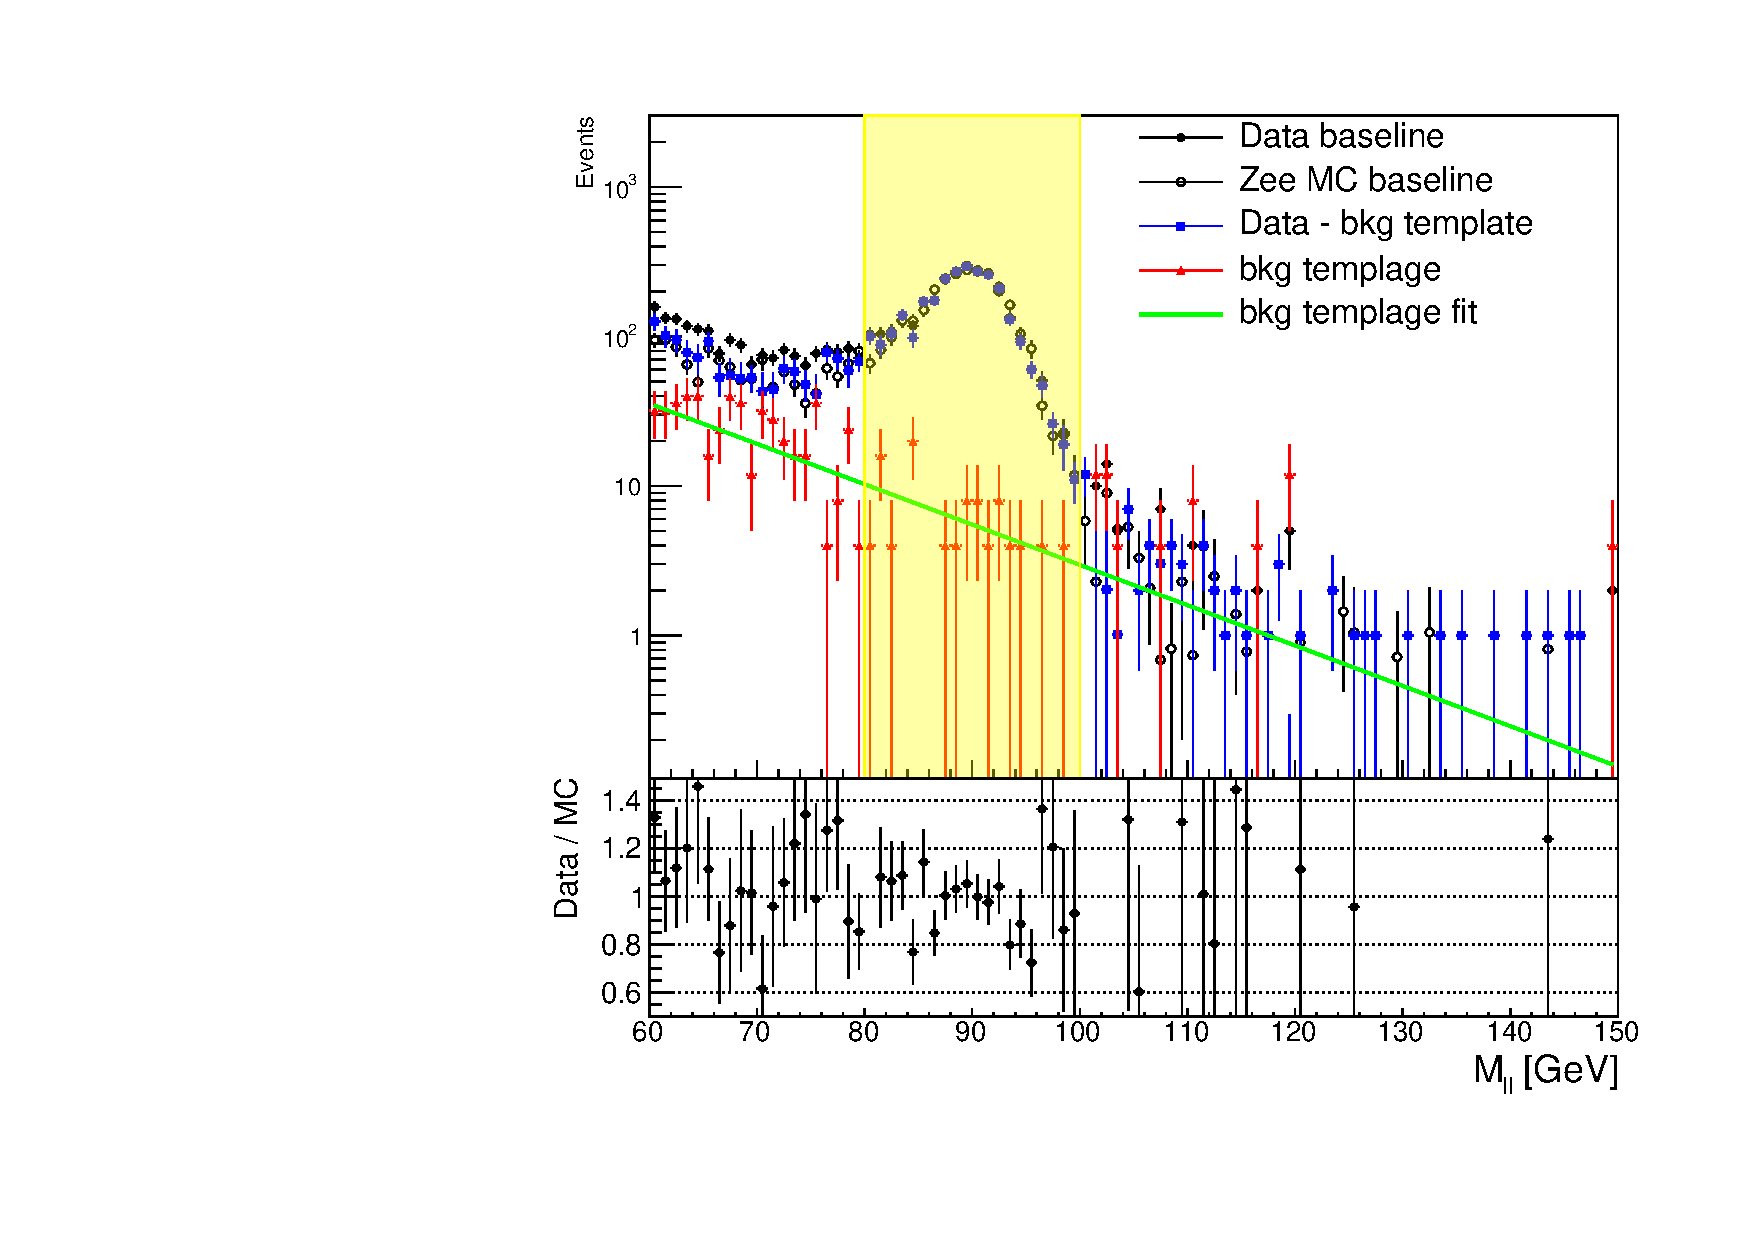
\includegraphics[scale=0.27]{bkg_subtraction_baseline_template_range_baseline_mll80_100_pt10_15_eta0_80_tag_trigger_matched.pdf}
            \caption{$10 < \pt < 15$~{\GeV}\\$0 < |\eta| < 0.8$}
        \end{center}
    \end{subfigure}
    \begin{subfigure}[b]{0.32\textwidth}
        \begin{center}
            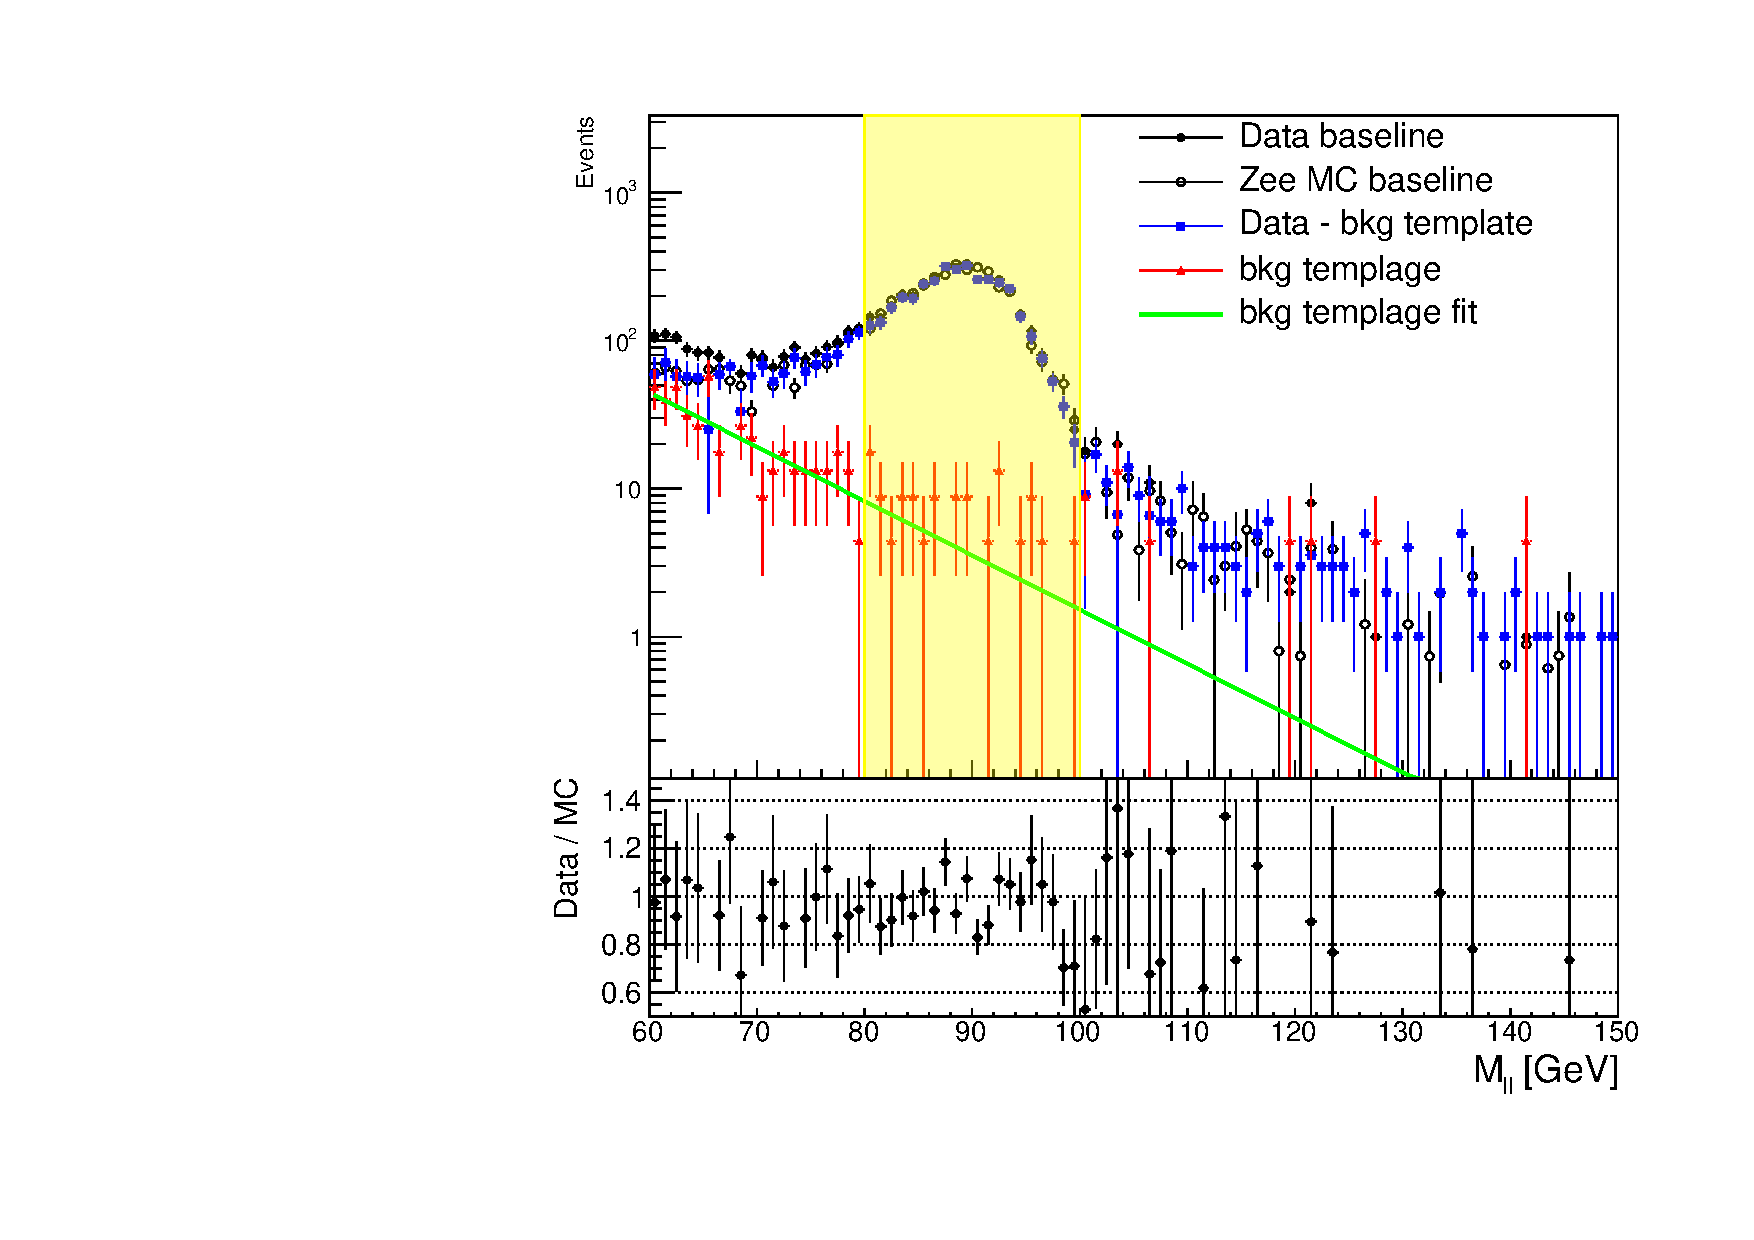
\includegraphics[scale=0.27]{bkg_subtraction_baseline_template_range_baseline_mll80_100_pt10_15_eta80_137_tag_trigger_matched.pdf}
            \caption{$10 < \pt < 15$~{\GeV}\\$0.8 < |\eta| < 1.37$}
        \end{center}
    \end{subfigure}
    \begin{subfigure}[b]{0.32\textwidth}
        \begin{center}
            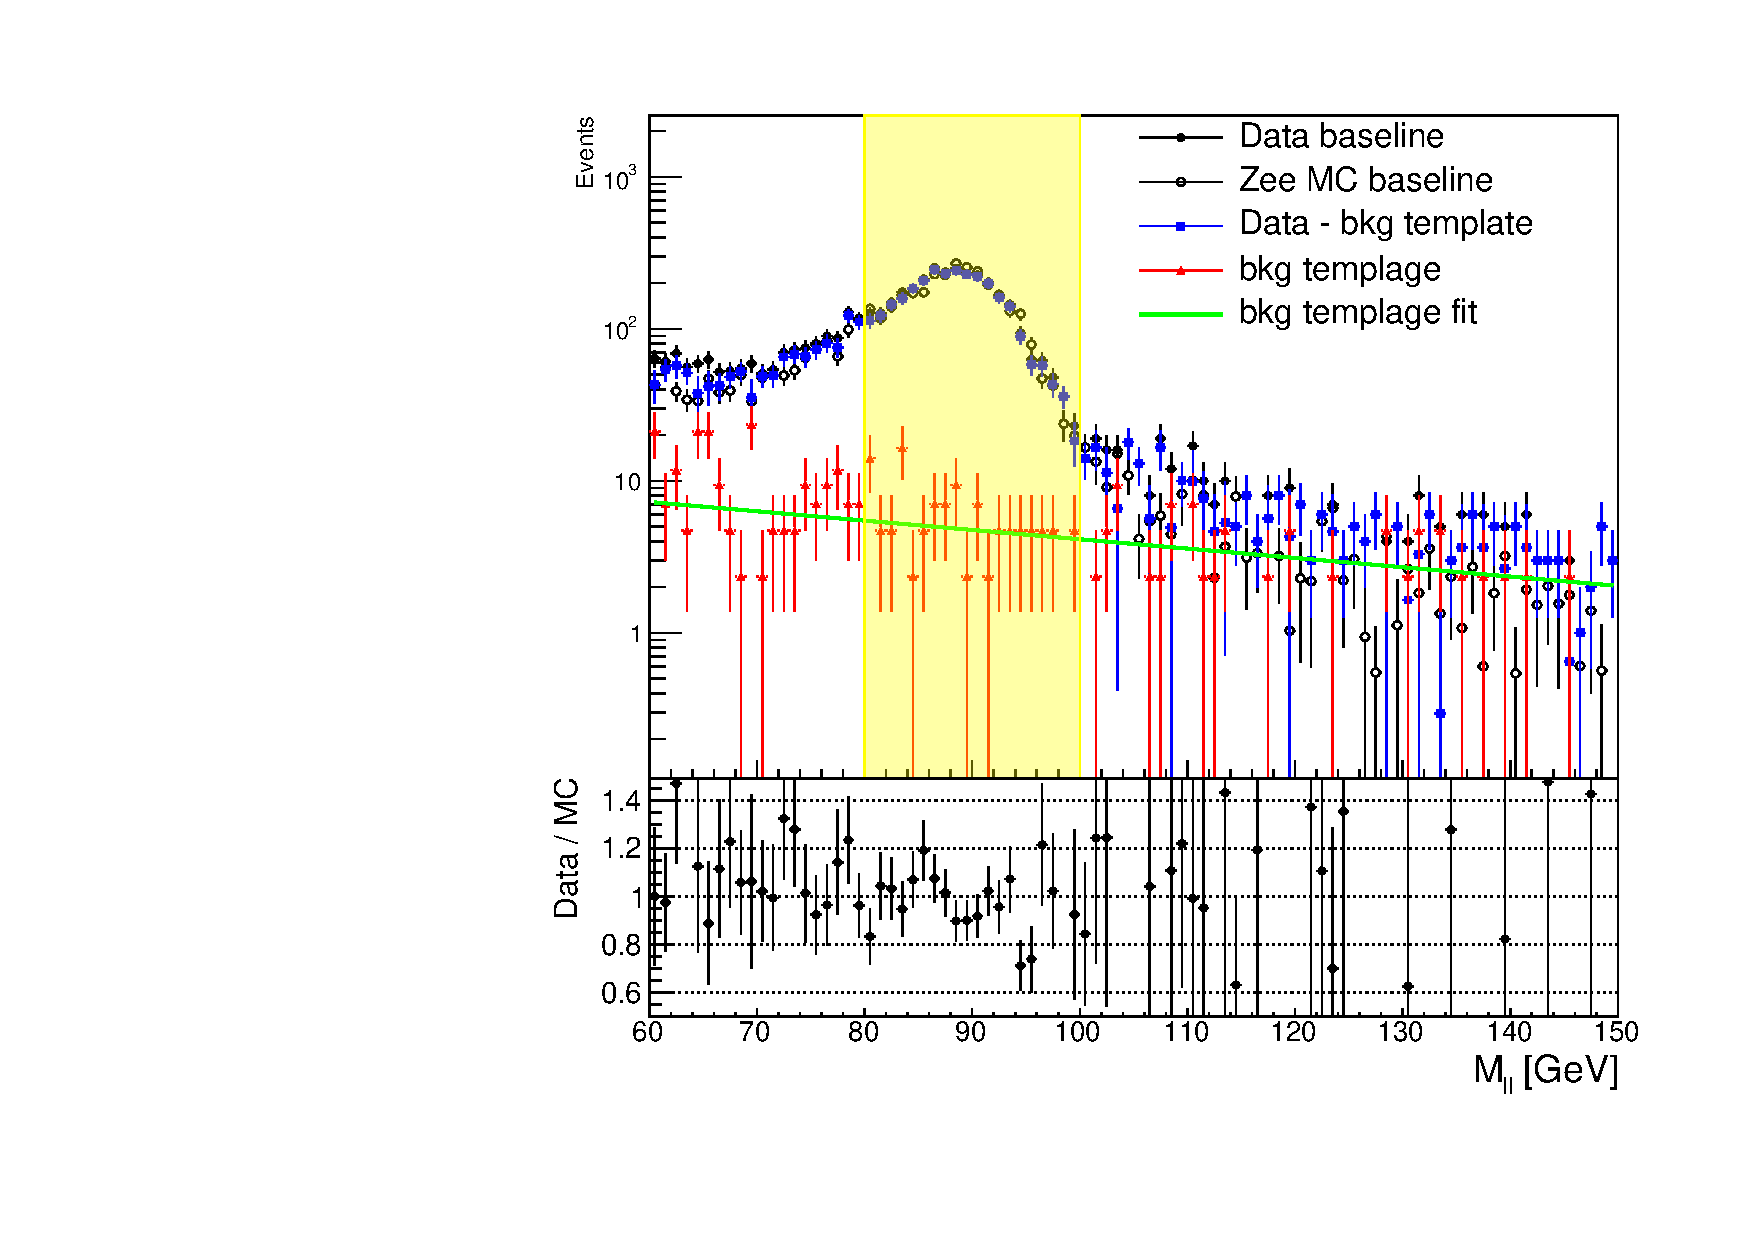
\includegraphics[scale=0.27]{bkg_subtraction_baseline_template_range_baseline_mll80_100_pt10_15_eta151_200_tag_trigger_matched.pdf}
            \caption{$10 < \pt < 15$~{\GeV}\\$1.52 < |\eta| < 2.0$}
        \end{center}
    \end{subfigure}
    \\
    \begin{subfigure}[b]{0.32\textwidth}
        \begin{center}
            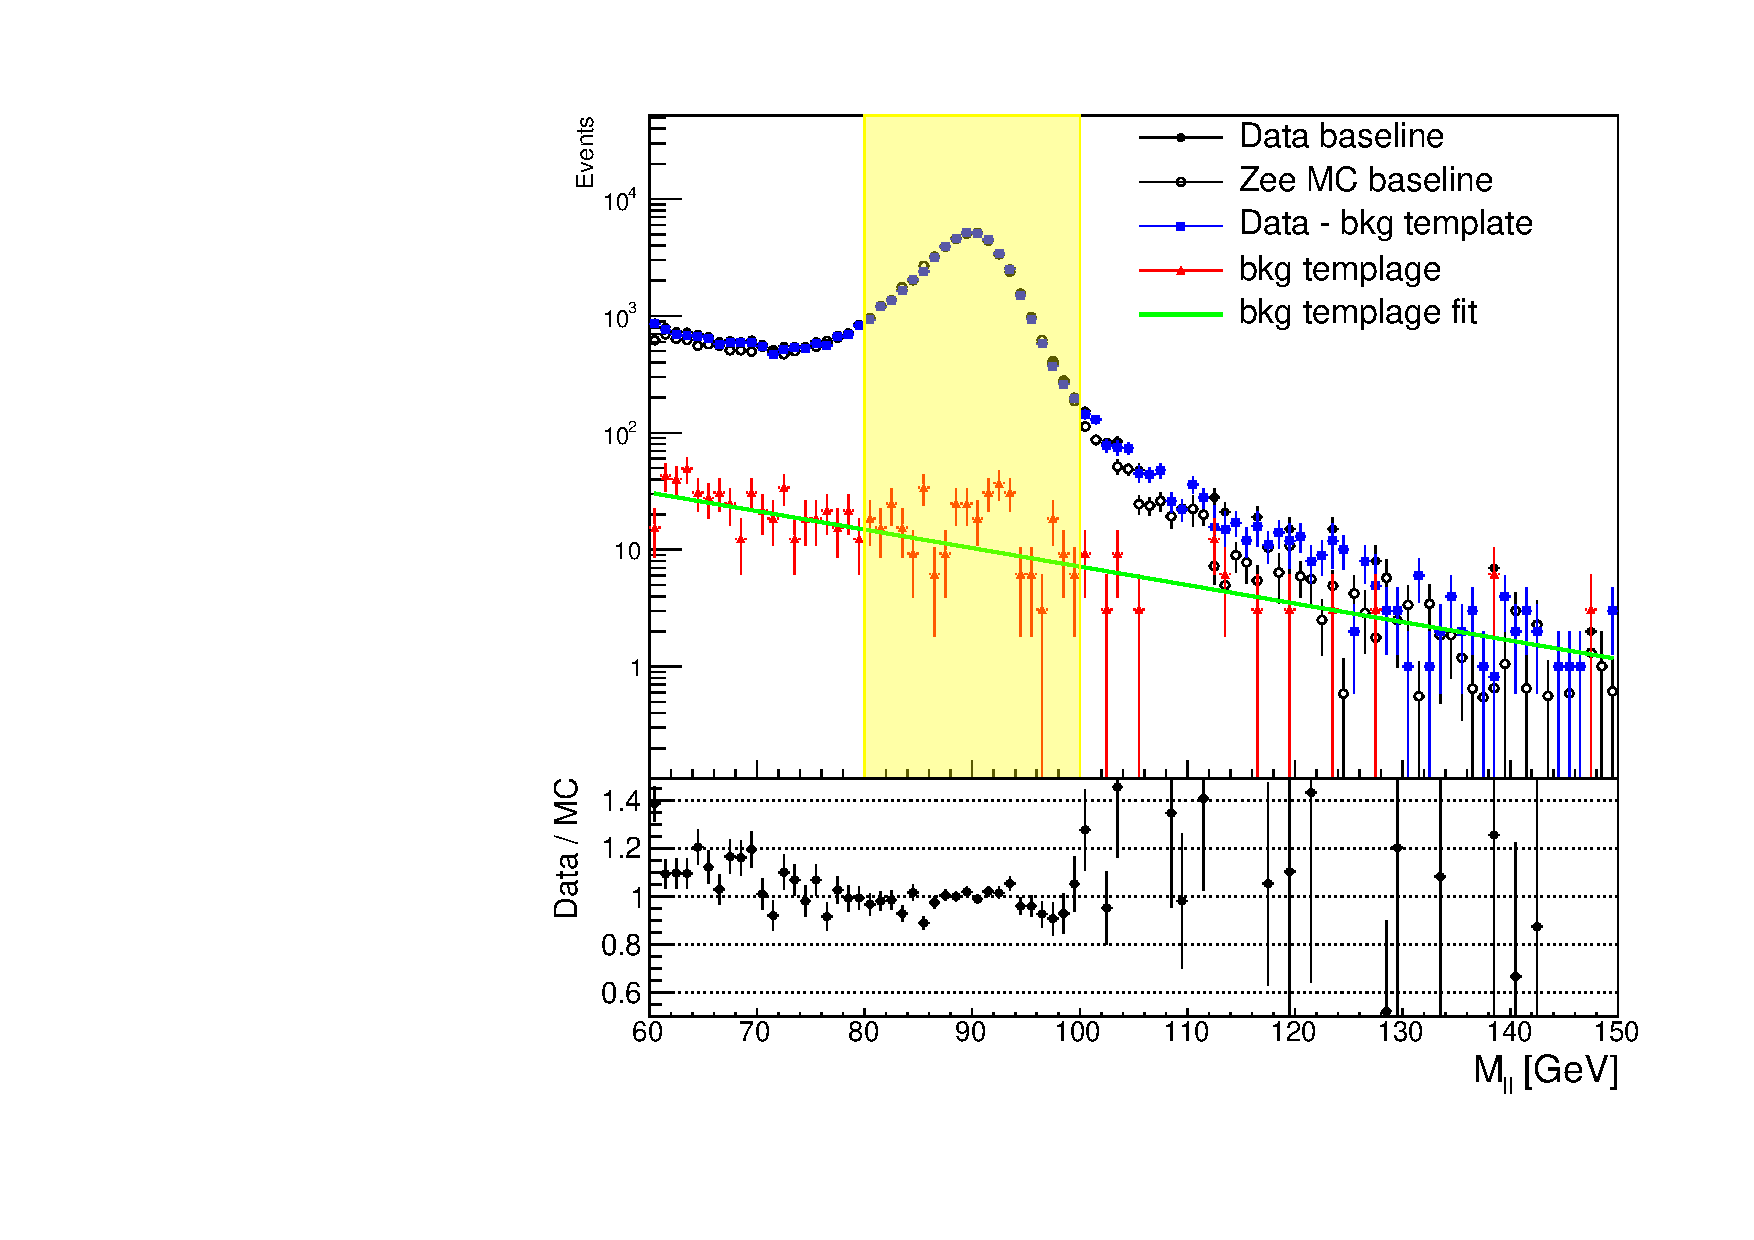
\includegraphics[scale=0.27]{bkg_subtraction_baseline_template_range_baseline_mll80_100_pt15_20_eta0_80_tag_trigger_matched.pdf}
            \caption{$15 < \pt < 20$~{\GeV}\\$0 < |\eta| < 0.8$}
        \end{center}
    \end{subfigure}
    \begin{subfigure}[b]{0.32\textwidth}
        \begin{center}
            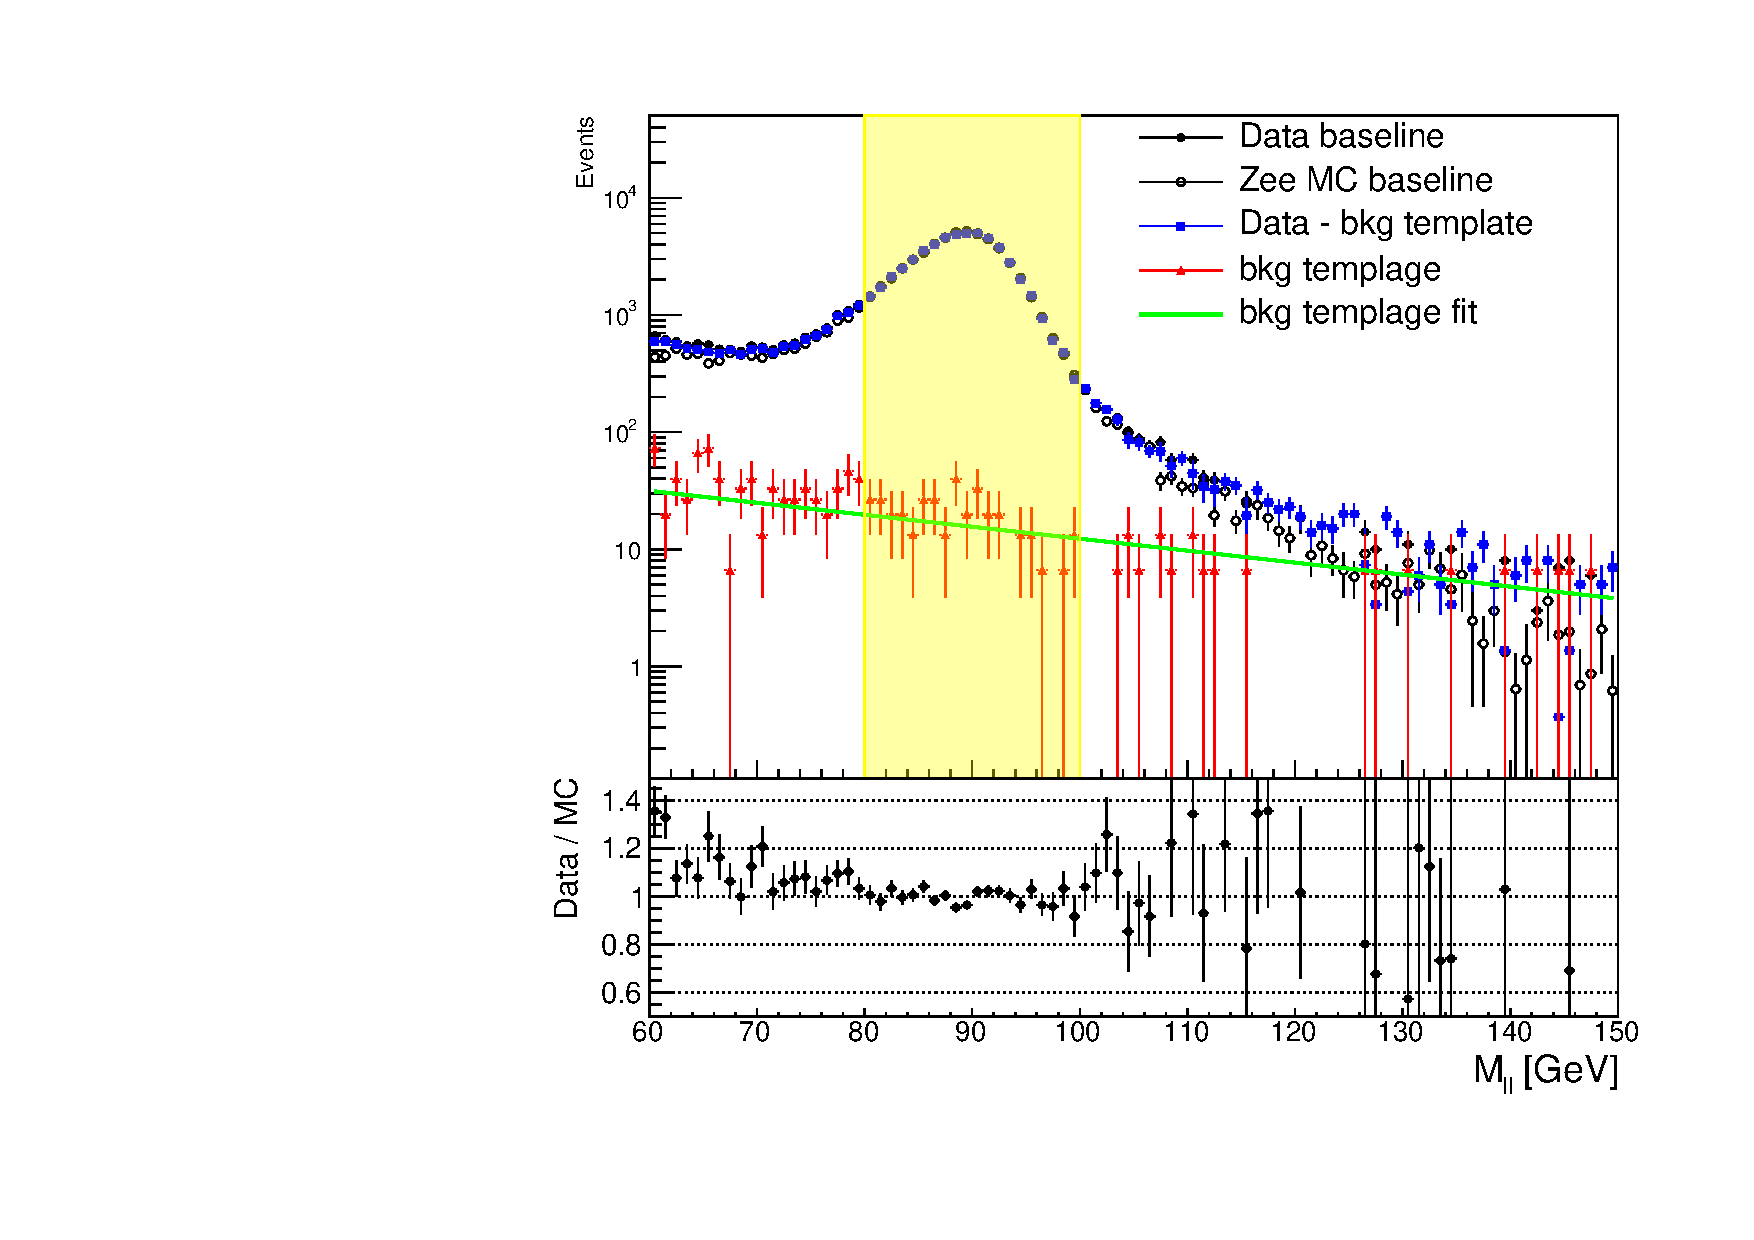
\includegraphics[scale=0.27]{bkg_subtraction_baseline_template_range_baseline_mll80_100_pt15_20_eta80_137_tag_trigger_matched.pdf}
            \caption{$15 < \pt < 20$~{\GeV}\\$0.8 < |\eta| < 1.37$}
        \end{center}
    \end{subfigure}
    \begin{subfigure}[b]{0.32\textwidth}
        \begin{center}
            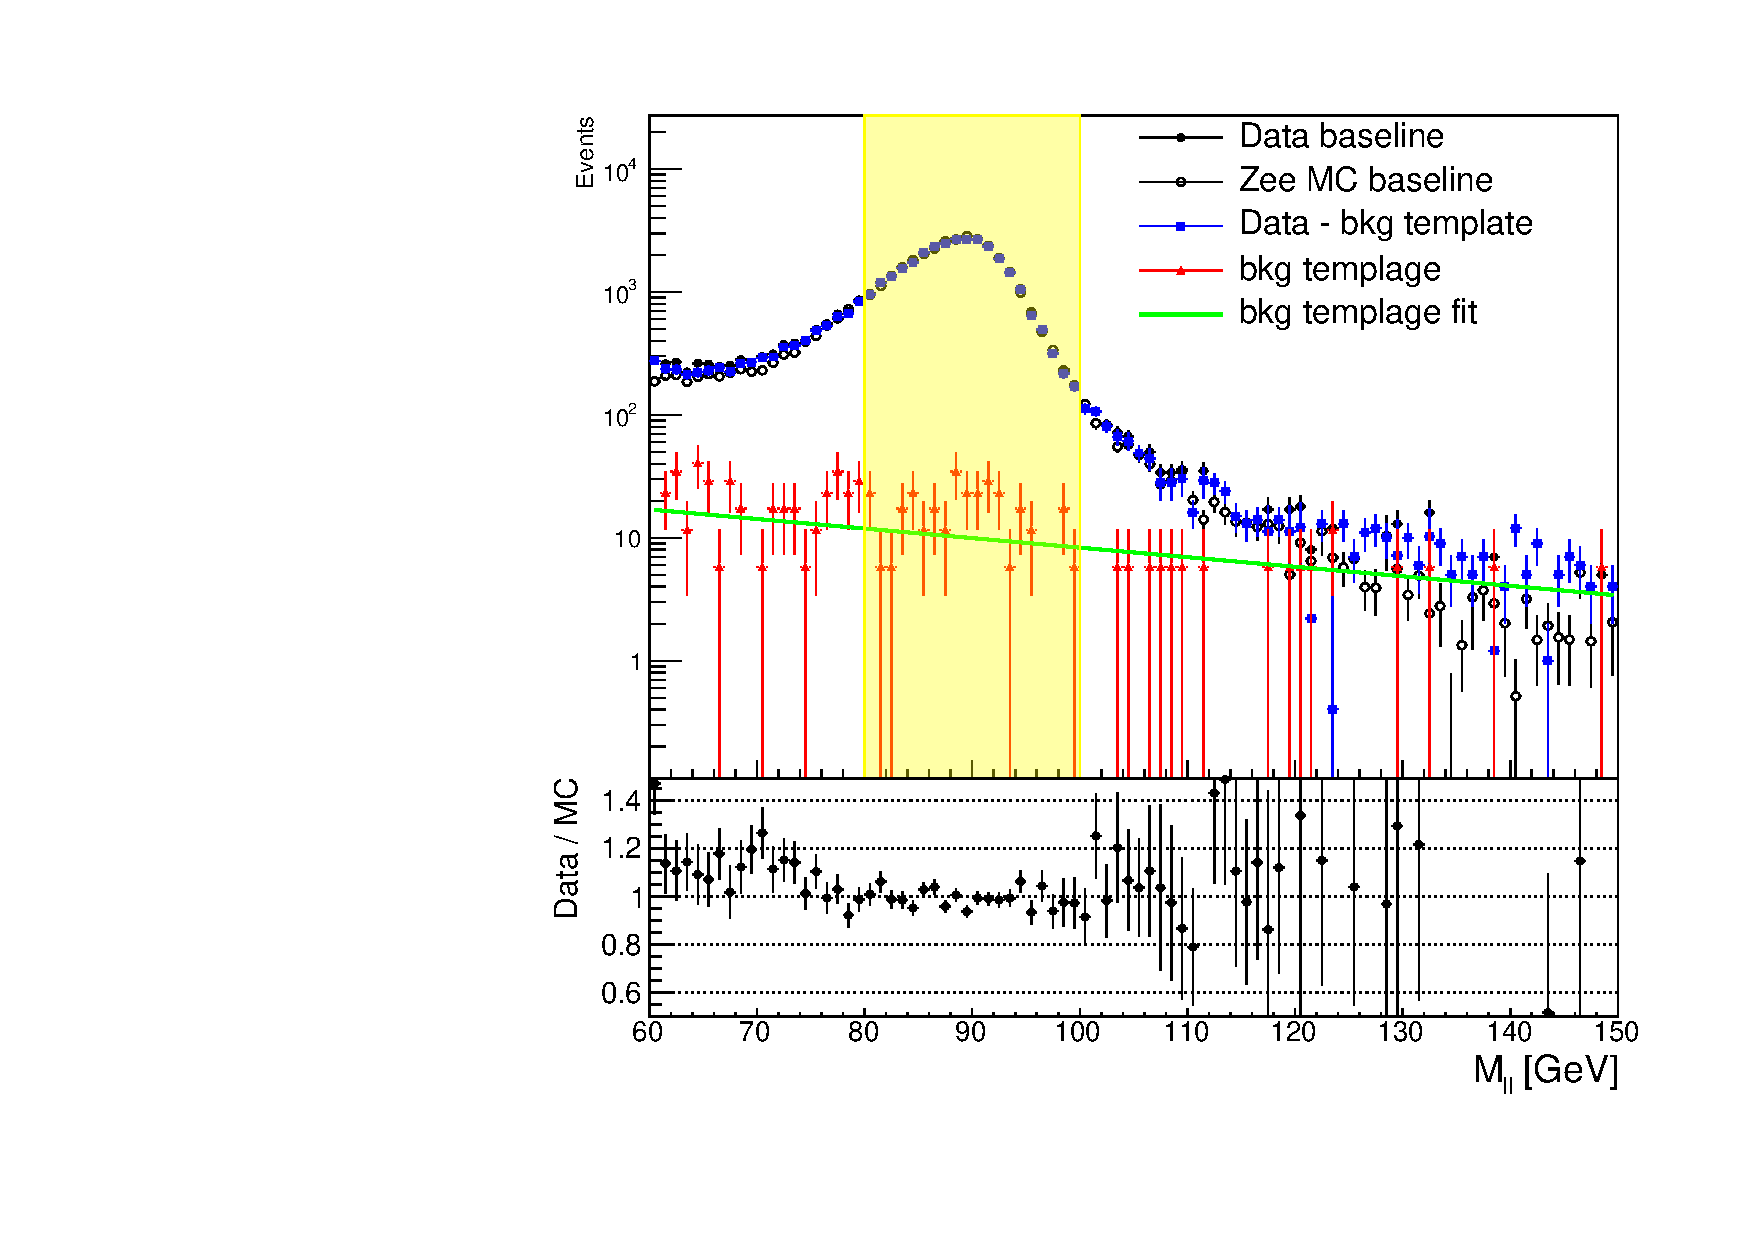
\includegraphics[scale=0.27]{bkg_subtraction_baseline_template_range_baseline_mll80_100_pt15_20_eta151_200_tag_trigger_matched.pdf}
            \caption{$15 < \pt < 20$~{\GeV}\\$1.52<|\eta|<2.0$}
        \end{center}
    \end{subfigure}
    \caption{Illustration of the background subtraction procedure.
    The full black dots and blue squares are the $m_{ee}$ distributions for data before and after performing the background subtraction, respectively.
    The $m_{ee}$ distribution for $Z \to ee$ MC, which is labeled by the open black circles, is normalized to the data after the background subtraction using a Gaussian fit of $85 < m_{ee} < 95$~{\GeV}.
    The lower panels show the data-to-MC ratio where the background subtraction has been applied on data.
    The background templates and their respective fitting results are indicated by the red triangles and green lines, respectively.
    }
    \label{fig:app_RLE_bkg_estimations}
\end{figure}
%
The data after performing the background subtraction, the MC simulation samples, the background template distributions, and the fitting results are also shown.
The simulated $m_{ee}$ distribution of $Z \to ee$ MC are normalized to the data, which background subtraction has been performed, using a Gaussian fit in $Z$ peak region $85 < m_{ee} < 95$~{\GeV}.
After performing the background subtraction, the data and MC have good agreement within the statistical uncertainties.

Then, the background contamination in the $Z$ mass region $80 < m_{ee} < 100$~{\GeV} is calculated using
%
\begin{equation}
    N_{bkg}^{80 < m_{ee} < 100~{\GeV}} = \int_{80}^{100} N_\mathrm{template} \ dm_{ee} \cdot \frac{N_{bkg}^\mathrm{tail}}{N_\mathrm{template}^\mathrm{tail}}
    \label{eq:RLE_bkg_in_80_mll_100}
\end{equation}
%
Table~\ref{tab:app_RLE_bkg_estimations} summarize the background estimations in different \pt and $|\eta|$ regions.
%
\begin{table}[htb]
    \begin{center}
        \begin{tabular}{cccc}
            \hline
            \hline
                                  & $0 < |\eta| < 0.8$ & $0.8 < |\eta| < 1.37$ & $1.52 < |\eta| < 2.0$\\
            \hline
            $10< \pt < 15$~{\GeV} & 4.04\%             & 2.10\%                & 3.17\%\\
            $15< \pt < 20$~{\GeV} & 0.44\%             & 0.58\%                & 0.76\%\\
            \hline
            \hline
        \end{tabular}
    \end{center}
    \caption{The estimated background contamination in in different \pt and $|\eta|$ regions.
    The \pt and $|\eta|$ binnings correspond to the one used for the final measurements.}
    \label{tab:app_RLE_bkg_estimations}
\end{table}
%
The largest improvements are observed in the lowest \pt bin ($10 < \pt < 15$~{\GeV}) where a sizeable background contamination is subtracted.
The background contamination is relatively small in the second lowest \pt bin ($15 < \pt < 20$~{\GeV}) providing the evidence that high purity of prompt leptons can be obtained using $Z$ tag-and-probe method.
Table~\ref{tab:app_RLE_efficiency_before_and_after_background_subtraction} shows the real electron efficiencies before and after performing the background subtraction.

\begin{table}[htb]
    %\begin{center}
    \resizebox{\textwidth}{!}{% <------ Don't forget this %
        \begin{tabular}{ccccc}
            \hline
            \hline
                                                    & background subtraction & $0 < |\eta| < 0.8$ & $0.8 < |\eta| < 1.37$ & $1.52 <| \eta| < 2.0$\\
            \hline
            \multirow{2}{*}{$10 < \pt < 15$~{\GeV}} & before                 & $57.4 \pm 0.9$     & $66.6 \pm 0.8$        & $53.2 \pm 0.9$\\
                                                    & after                  & $59.9 \pm 1.9$     & $68.0 \pm 1.8$        & $55.0 \pm 1.7$\\
            \hline
            \multirow{2}{*}{$15 < \pt < 20$~{\GeV}} & before                 & $64.5 \pm 0.2$     & $69.4 \pm 0.2$        & $62.0 \pm 0.3$\\
                                                    & after                  & $64.8 \pm 0.5$     & $69.8 \pm 0.5$        & $62.5 \pm 0.6$\\
            \hline
            \hline
        \end{tabular}
    }
    %\end{center}
    \caption{The real electron efficiencies before and after performing the background subtraction in different \pt and $|\eta|$ regions are shown in percentage.}
    \label{tab:app_RLE_efficiency_before_and_after_background_subtraction}
\end{table}

%%%
%%%
%%%

\section{Cut efficiencies}
\label{sec:app_RLE_cut_efficiencies}
Figure~\ref{fig:app_RLE_cut_efficiencies} shows the efficiencies associated to each signal cut with respect to baseline definitions.
%
\begin{figure}[htb]
    \begin{subfigure}[b]{0.48\textwidth}
        \begin{center}
            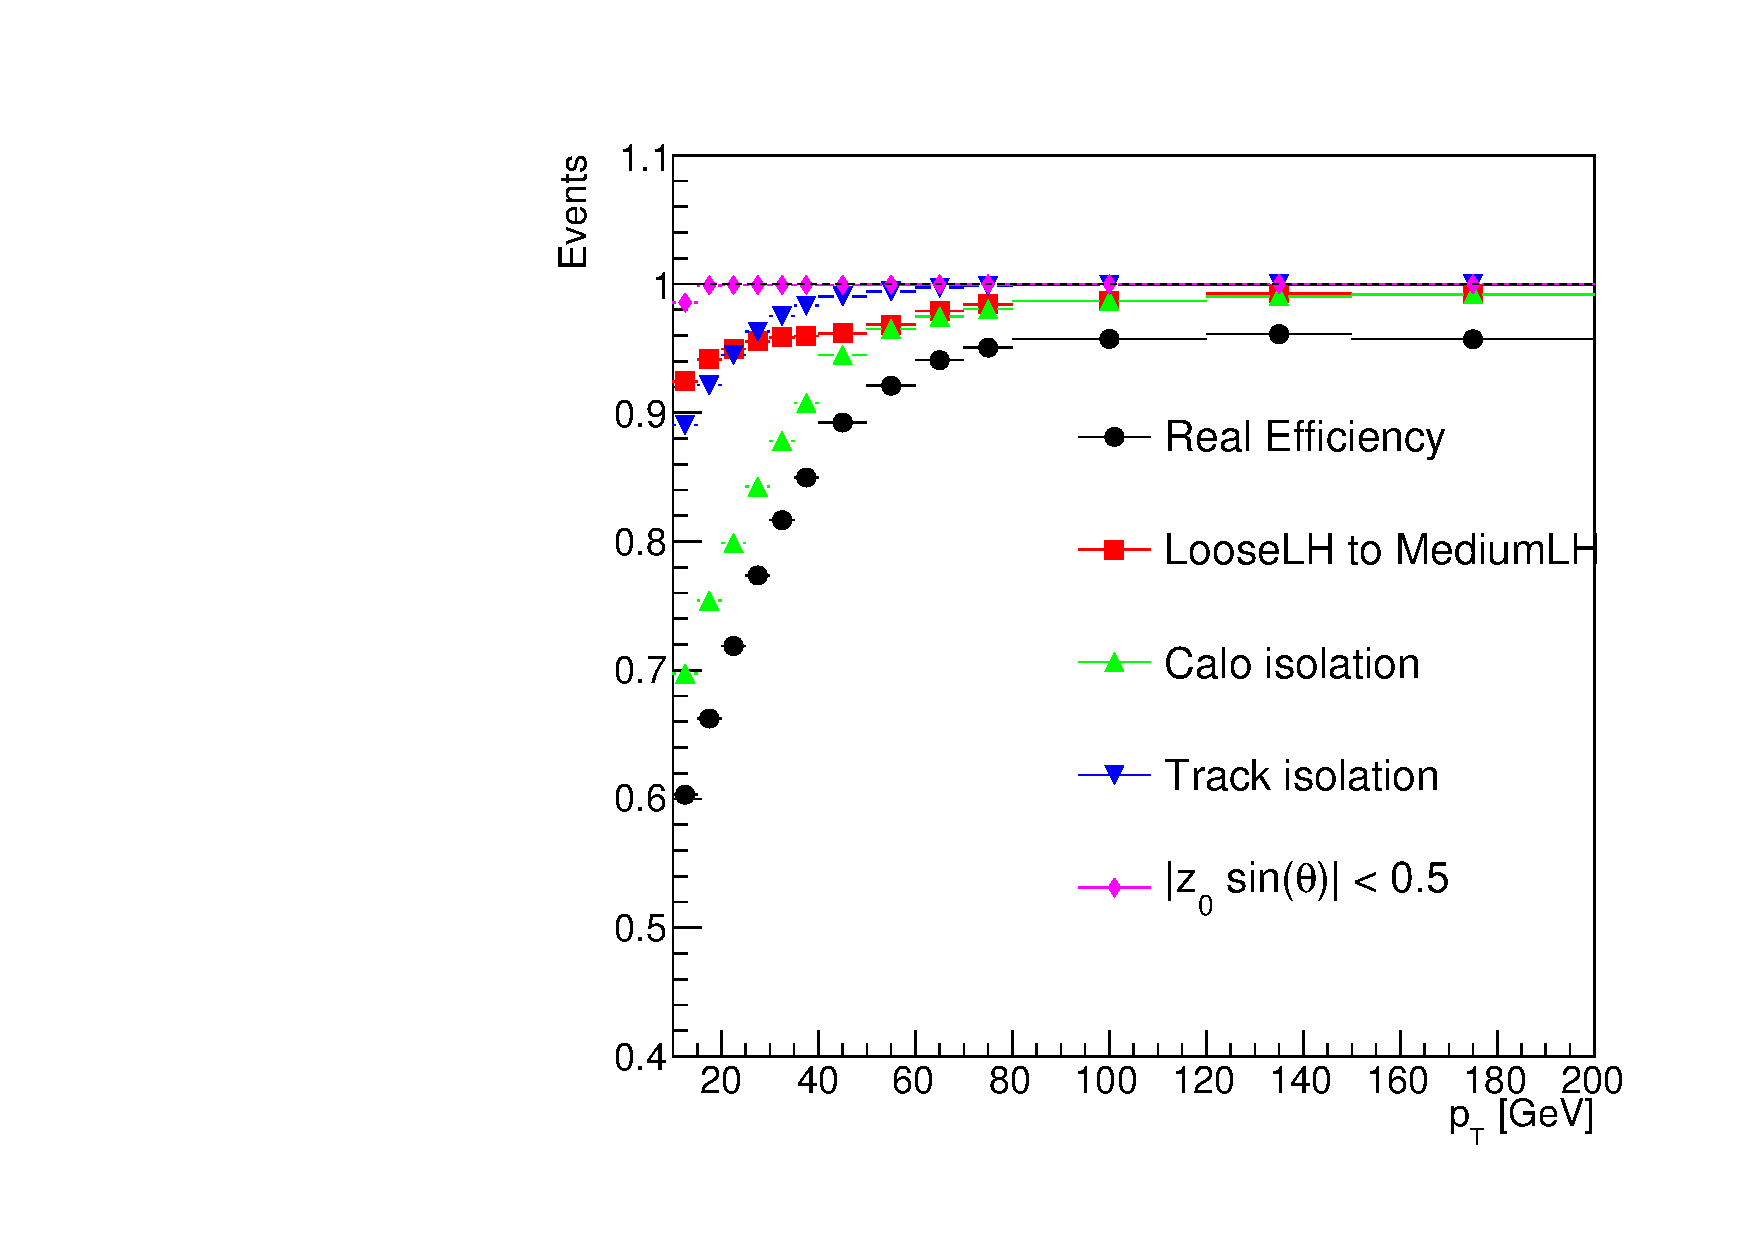
\includegraphics[scale=0.4]{cut_efficiency_electron.pdf}
            \caption{Electron}
        \end{center}
    \end{subfigure}
    \begin{subfigure}[b]{0.48\textwidth}
        \begin{center}
            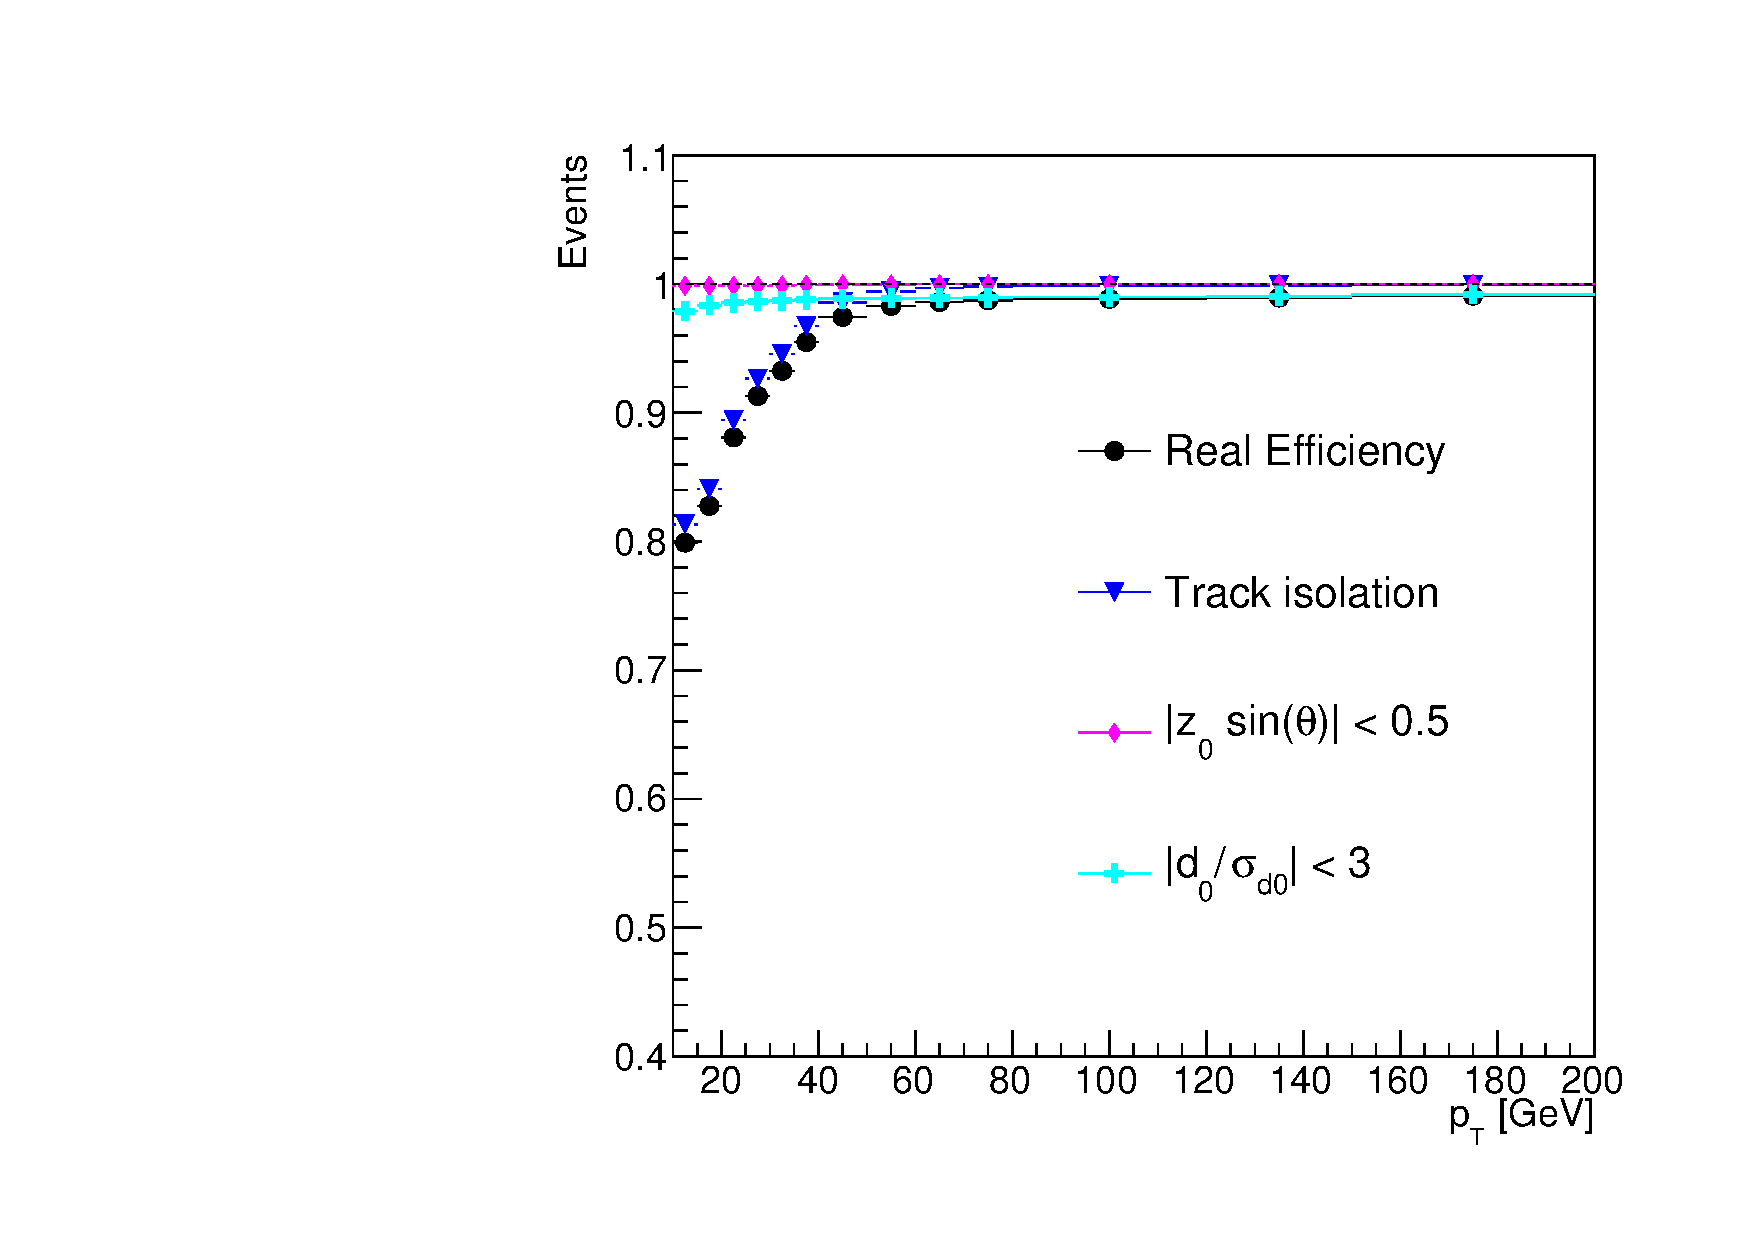
\includegraphics[scale=0.4]{cut_efficiency_muon.pdf}
            \caption{Muon}
        \end{center}
    \end{subfigure}
    \caption{Cut efficiencies of the signal electron and muon definition as a function of \pt.
    The total real electron and muon efficiencies are presented by black points. 
    The loose to medium likelihood cut efficiency is presented by red squares.
    The calorimeter and track isolation cut efficiencies are presented by green triangles and blue triangles, respectvely.
    The longitudinal and tranverse impact parameters cut efficiencies are presented by magenta diamonds and cyan crosses, respectively.}
    \label{fig:app_RLE_cut_efficiencies}
\end{figure}
%
The prompt electron efficiency increases with \pt from $\sim$62\% to $\sim$98\% and the efficiency losses are dominated by the calorimeter isolation.
The calorimeter isolation cut efficiency increases with \pt from $\sim$ 69\% to $\sim$98\%.
The loose to medium likelilihood (LH) cut efficiency increases from $\sim$92\% to $\sim$96\% in the $10< \pt < 30$~{\GeV} then reaches a plateau when $30 < \pt < 50$~{\GeV} and increases again to $\sim$98\% when $\pt > 60$~{\GeV}.
The track isolation cut efficiency increases from $\sim$89\% at low \pt to $\sim$100\% when $\pt > 60$~{\GeV}.
The longitudinal impact parameter cut efficiency increases from $\sim$98\% at low \pt to $\sim$100\% when $\pt > 15$~{\GeV}.
The cut efficiencies for muon are much higher than the electron case because the same muon identification is used for the baseline and the signal muon definitions.
The associated efficiencies computed using $Z\to \mu \mu$ events increase from $\sim$80\% for $10 < \pt < 15$~{\GeV} to $\sim$98\% when $\pt > 50$~{\GeV}.
The dominant contribution is the track isolation cut efficiency which increases from $\sim$82\% to 98\% when $\pt > 50$~{\GeV}.
The transverse and longitudinal impact parameter cut efficiencies are $\sim$99\% and 100\%, respectively.
For the electron case, the transverse impact parameter cut is already applied at the baseline level

%%%
%%%
%%%

\section{Real lepton efficiencies}
\label{sec:app_RLE}
The real lepton efficiencies as a function of \pt and $|\eta|$ are shown in Fig~\ref{fig:app_RLE_real_efficiency_total_systematics} where the background subtraction has been applied on the electron case in $10 < \pt < 15$~{\GeV} and $15 < \pt < 20$~{\GeV}.
%
\begin{figure}[htb]
    \begin{subfigure}[b]{0.48\textwidth}
        \begin{center}
            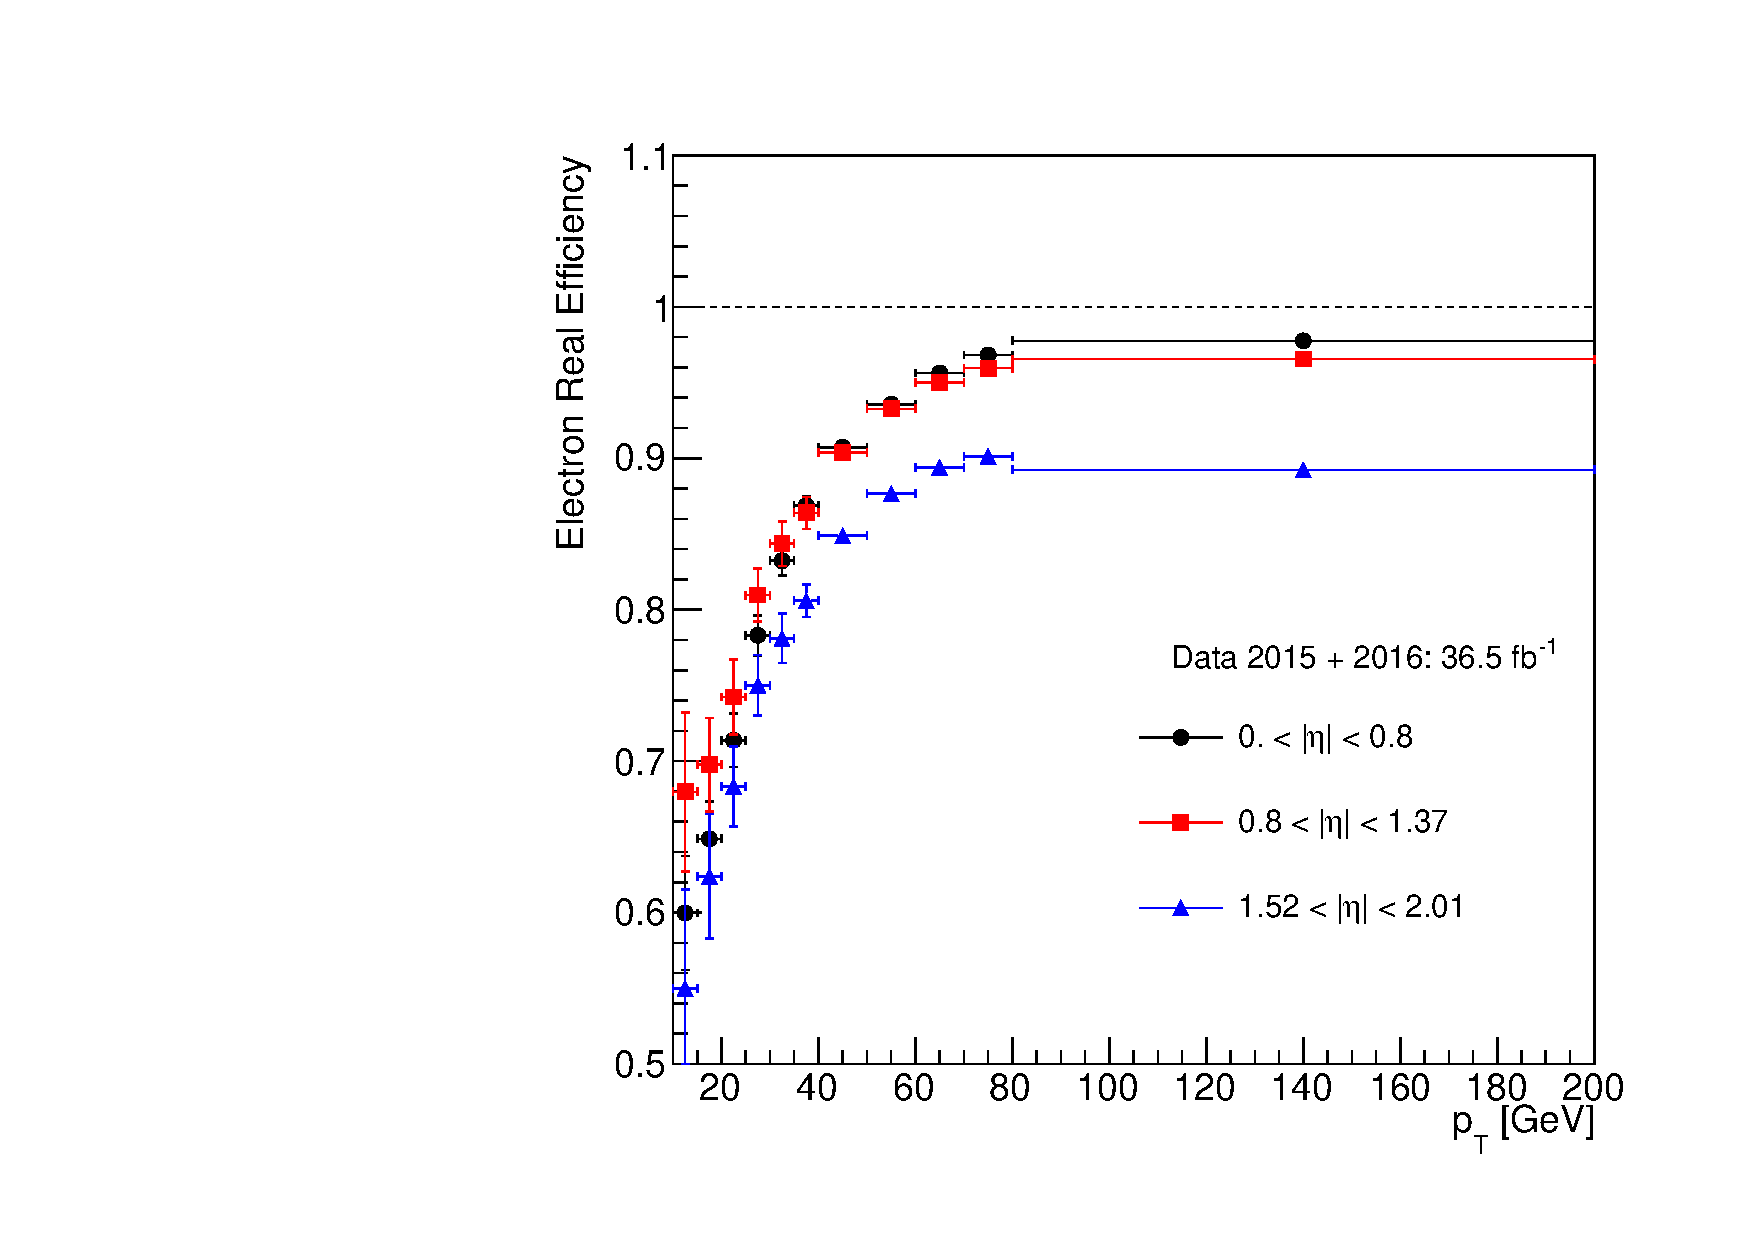
\includegraphics[scale=0.4]{real_electron_efficiency_total_systematics.pdf}
            \caption{Electron}
        \end{center}
    \end{subfigure}
    \begin{subfigure}[b]{0.48\textwidth}
        \begin{center}
            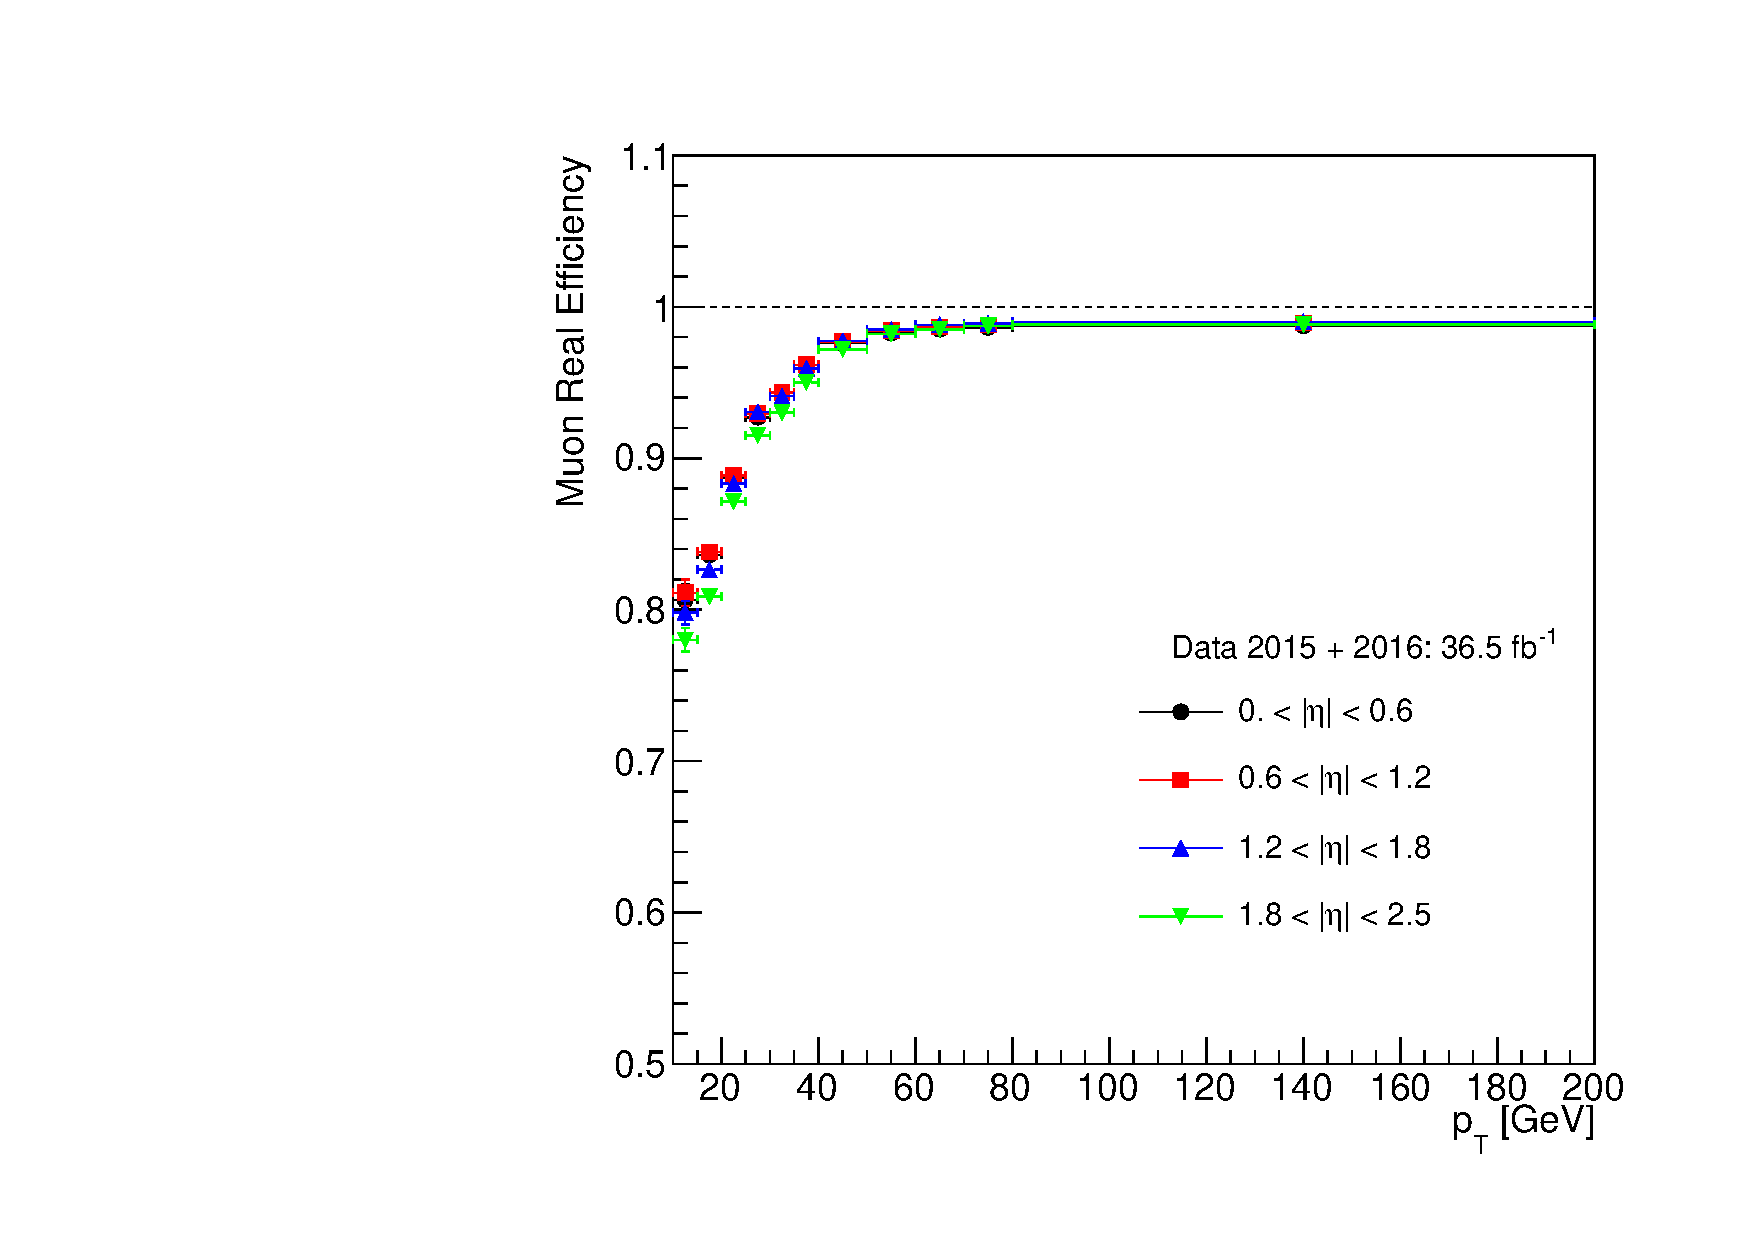
\includegraphics[scale=0.4]{real_muon_efficiency_total_systematics.pdf}
            \caption{Muon}
        \end{center}
    \end{subfigure}
    \caption{The real lepton efficiencies as a function of \pt and $|\eta|$ measured using the $Z$ tag-and-probe method.
    For the real electron efficiencies measurement, the $|\eta|$ binning in the creak region is removed.
    A homogeneous $|\eta|$ binnings are used for the muon case.}
    \label{fig:app_RLE_real_efficiency_total_systematics}
\end{figure}
%
The uncertainties are the quadratic sum of the statistical uncertainties and the measurement systematic uncertainties.
The 3 $|\eta|$ binnings for the electron case are driven by the geometry of ECAL.
The crack region, $1.37<|\eta|<1.52$, is removed from the real electron efficiency study.
It is expected that the electron efficiencies in $1.52<|\eta|<2.01$ are lower because the electron identification is better in the central region of the ECAL.

%%%
%%%
%%%

\subsection{Tag-and-probe method and truth matching comparisons}
\label{subsec:app_RLE_truth_matched}
The truth matched information in the $Z \to \ell \ell$ MC samples are used to verify the accuracy of $Z$ tag-and-probe method.
Figure~\ref{fig:app_RLE_TandP_truth_match_comparisons} shows the real lepton efficiencies as a function of \pt, $|\eta|$, and $\Delta R(\ell, \mathrm{jet})$ using $Z$ tag-and-probe method and truth matching.
%
\begin{figure}[htb]
    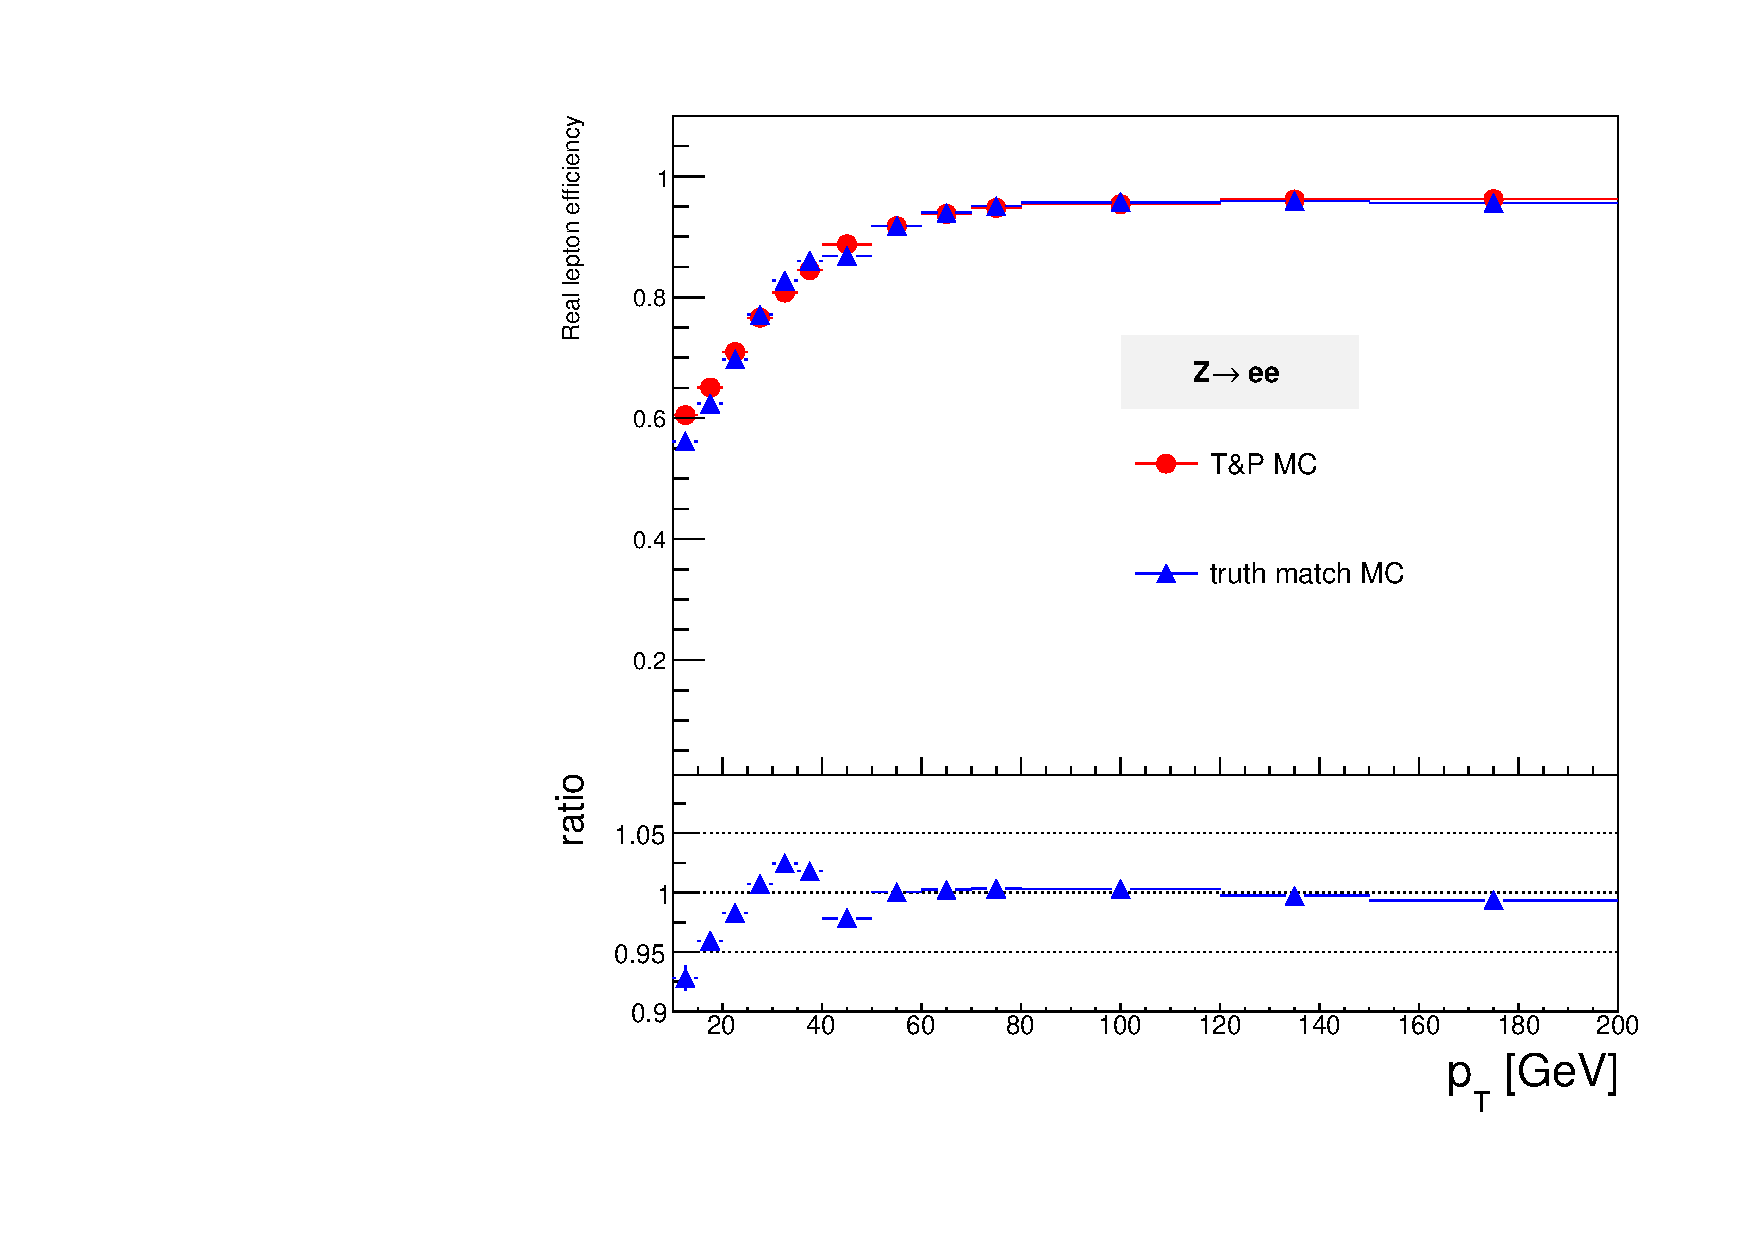
\includegraphics[width=0.33\textwidth]{Compare_TandP_truth_match_electron_pt.pdf}
    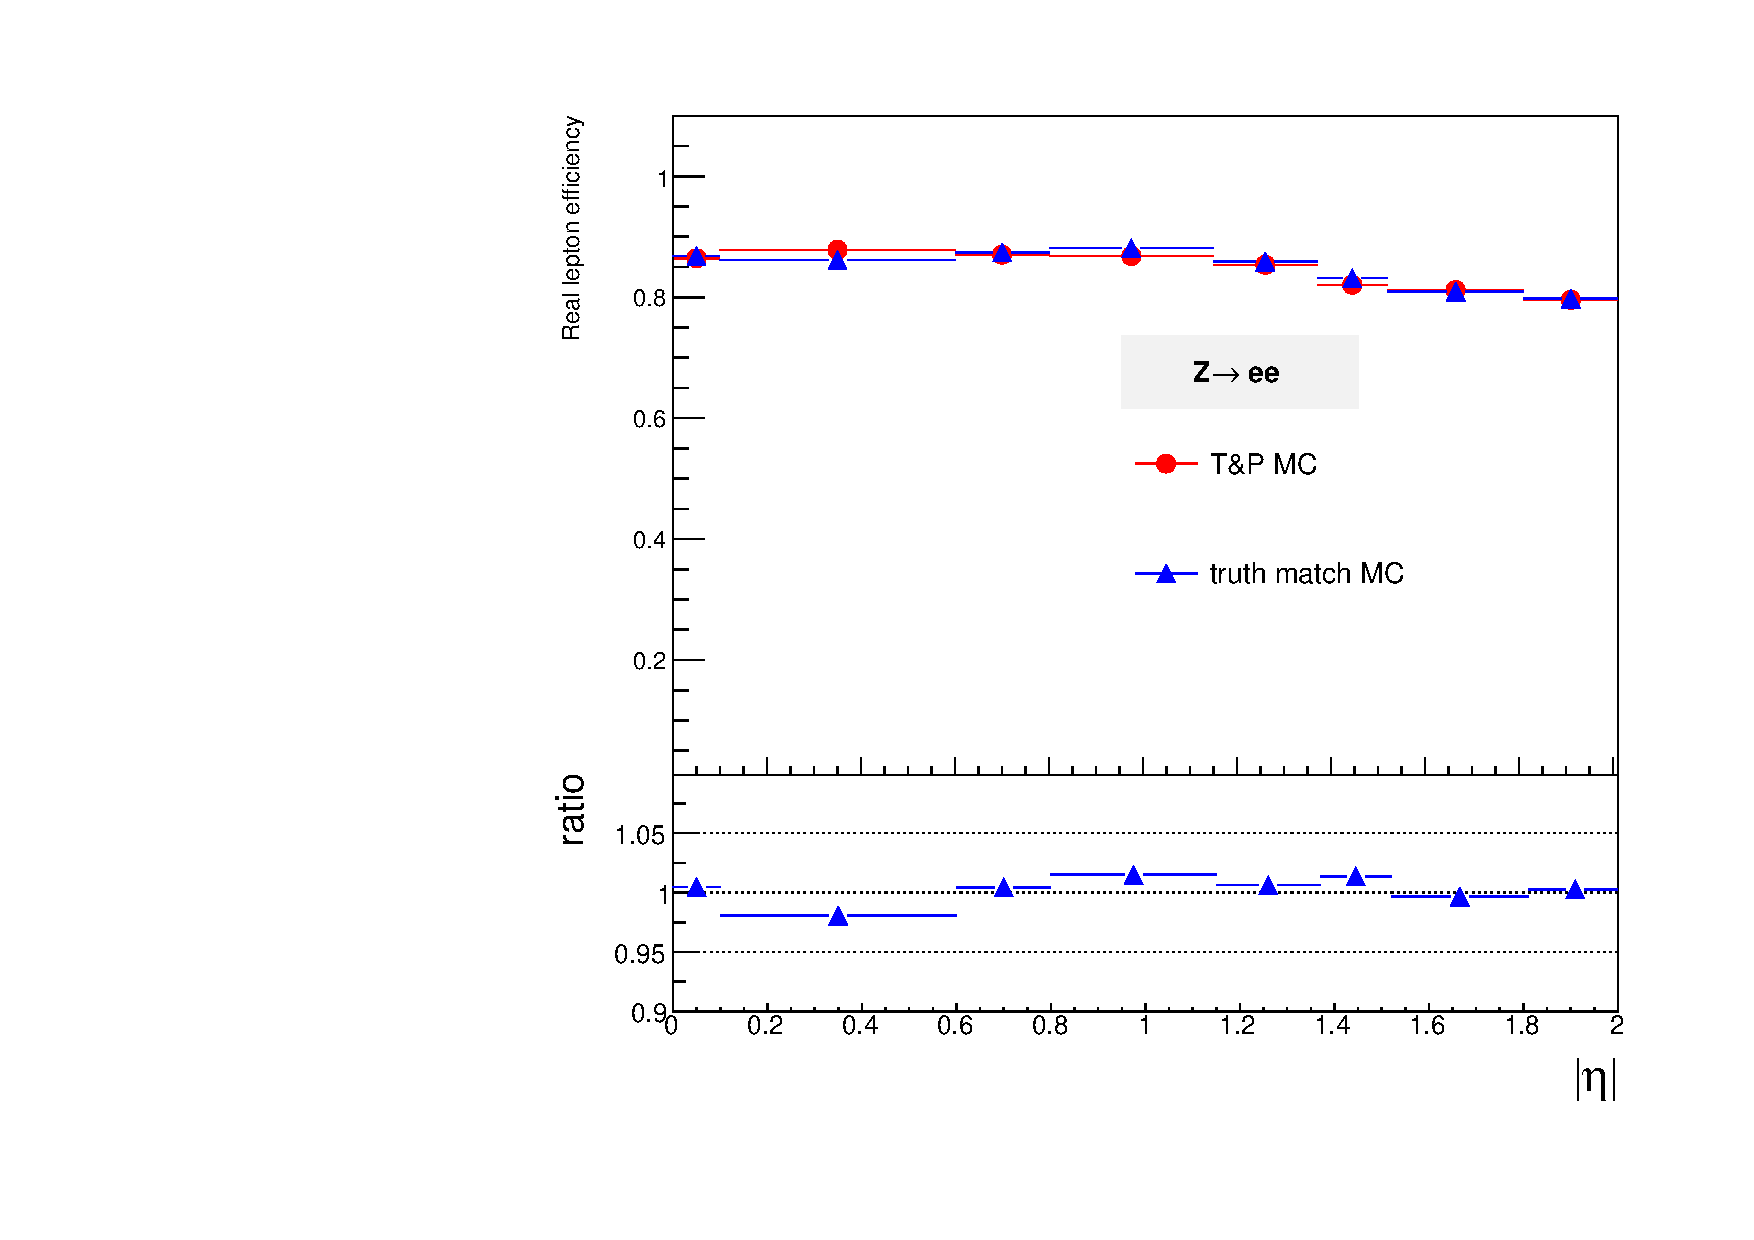
\includegraphics[width=0.33\textwidth]{Compare_TandP_truth_match_electron_eta.pdf}
    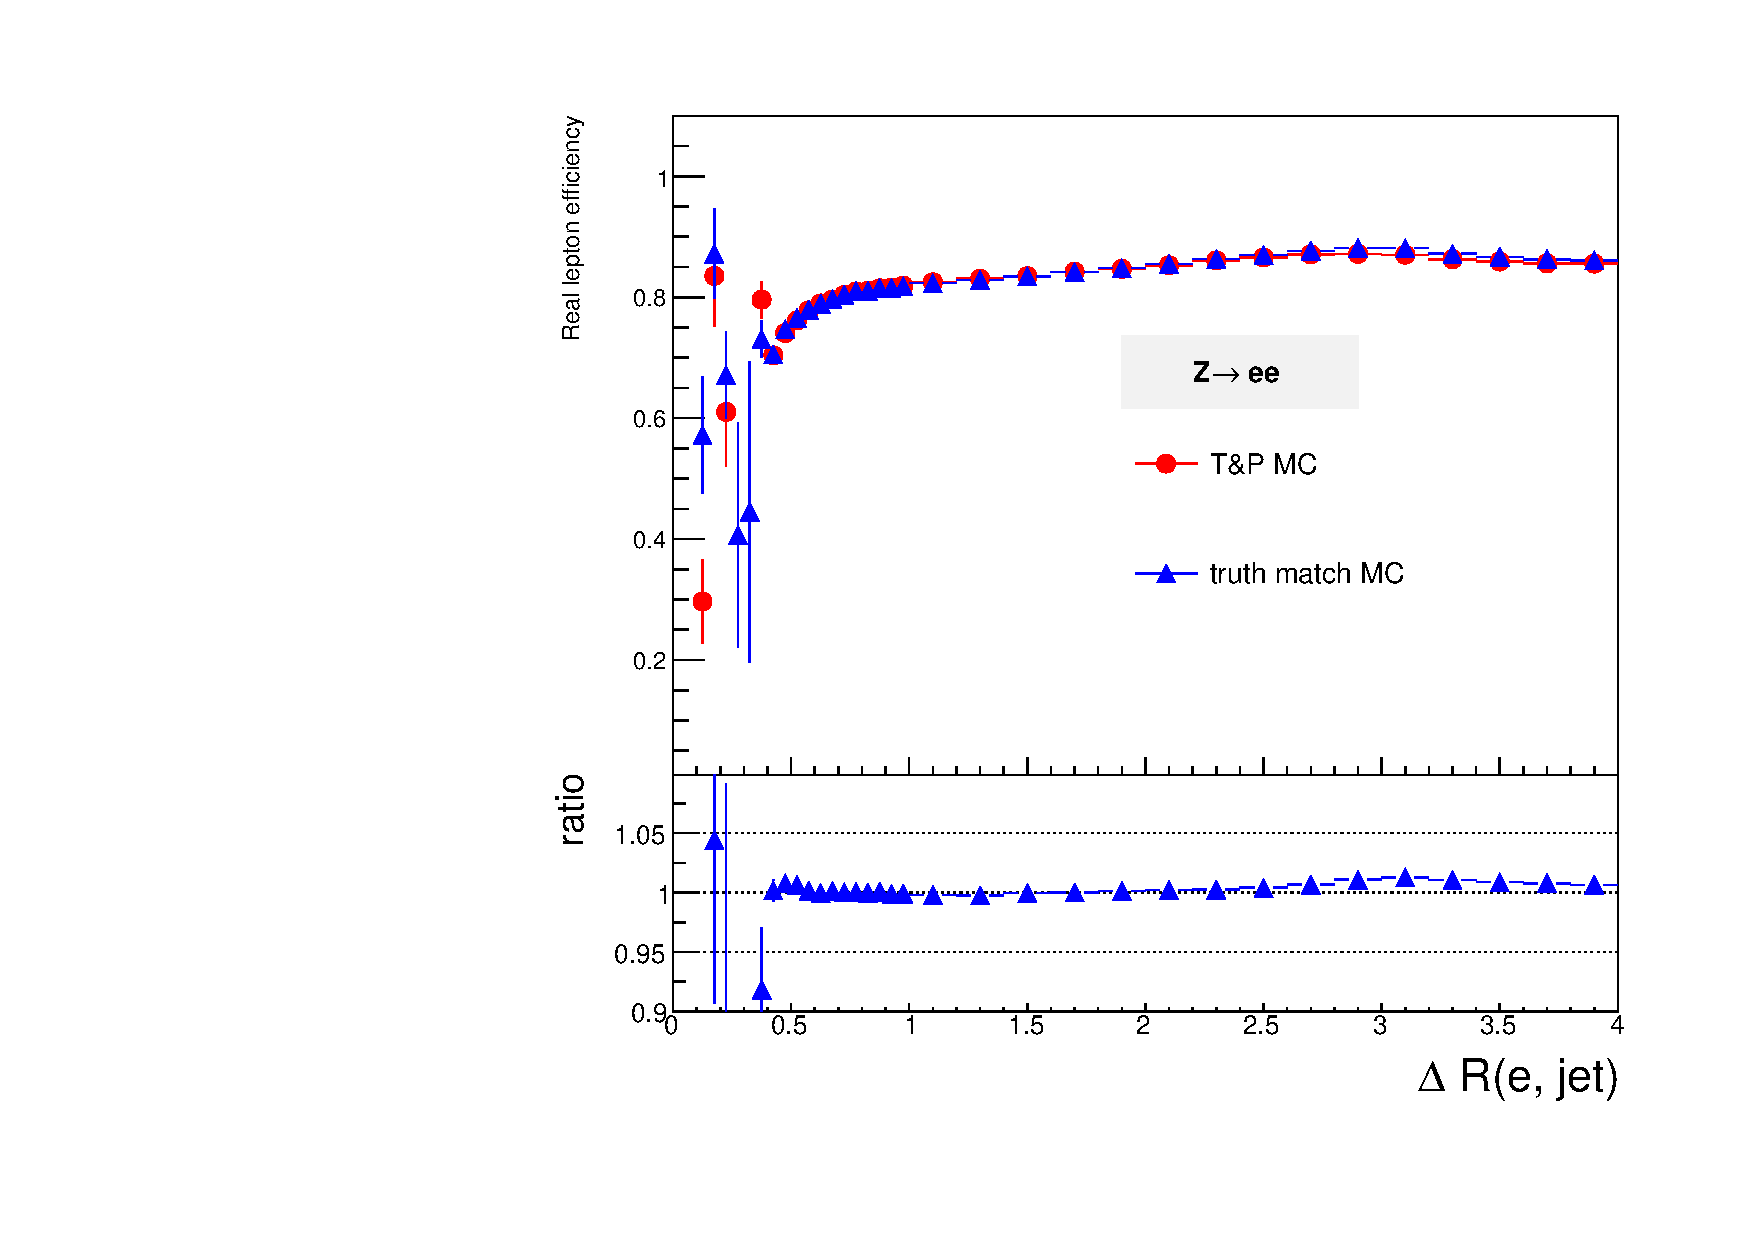
\includegraphics[width=0.33\textwidth]{Compare_TandP_truth_match_electron_dRjet.pdf}\\
    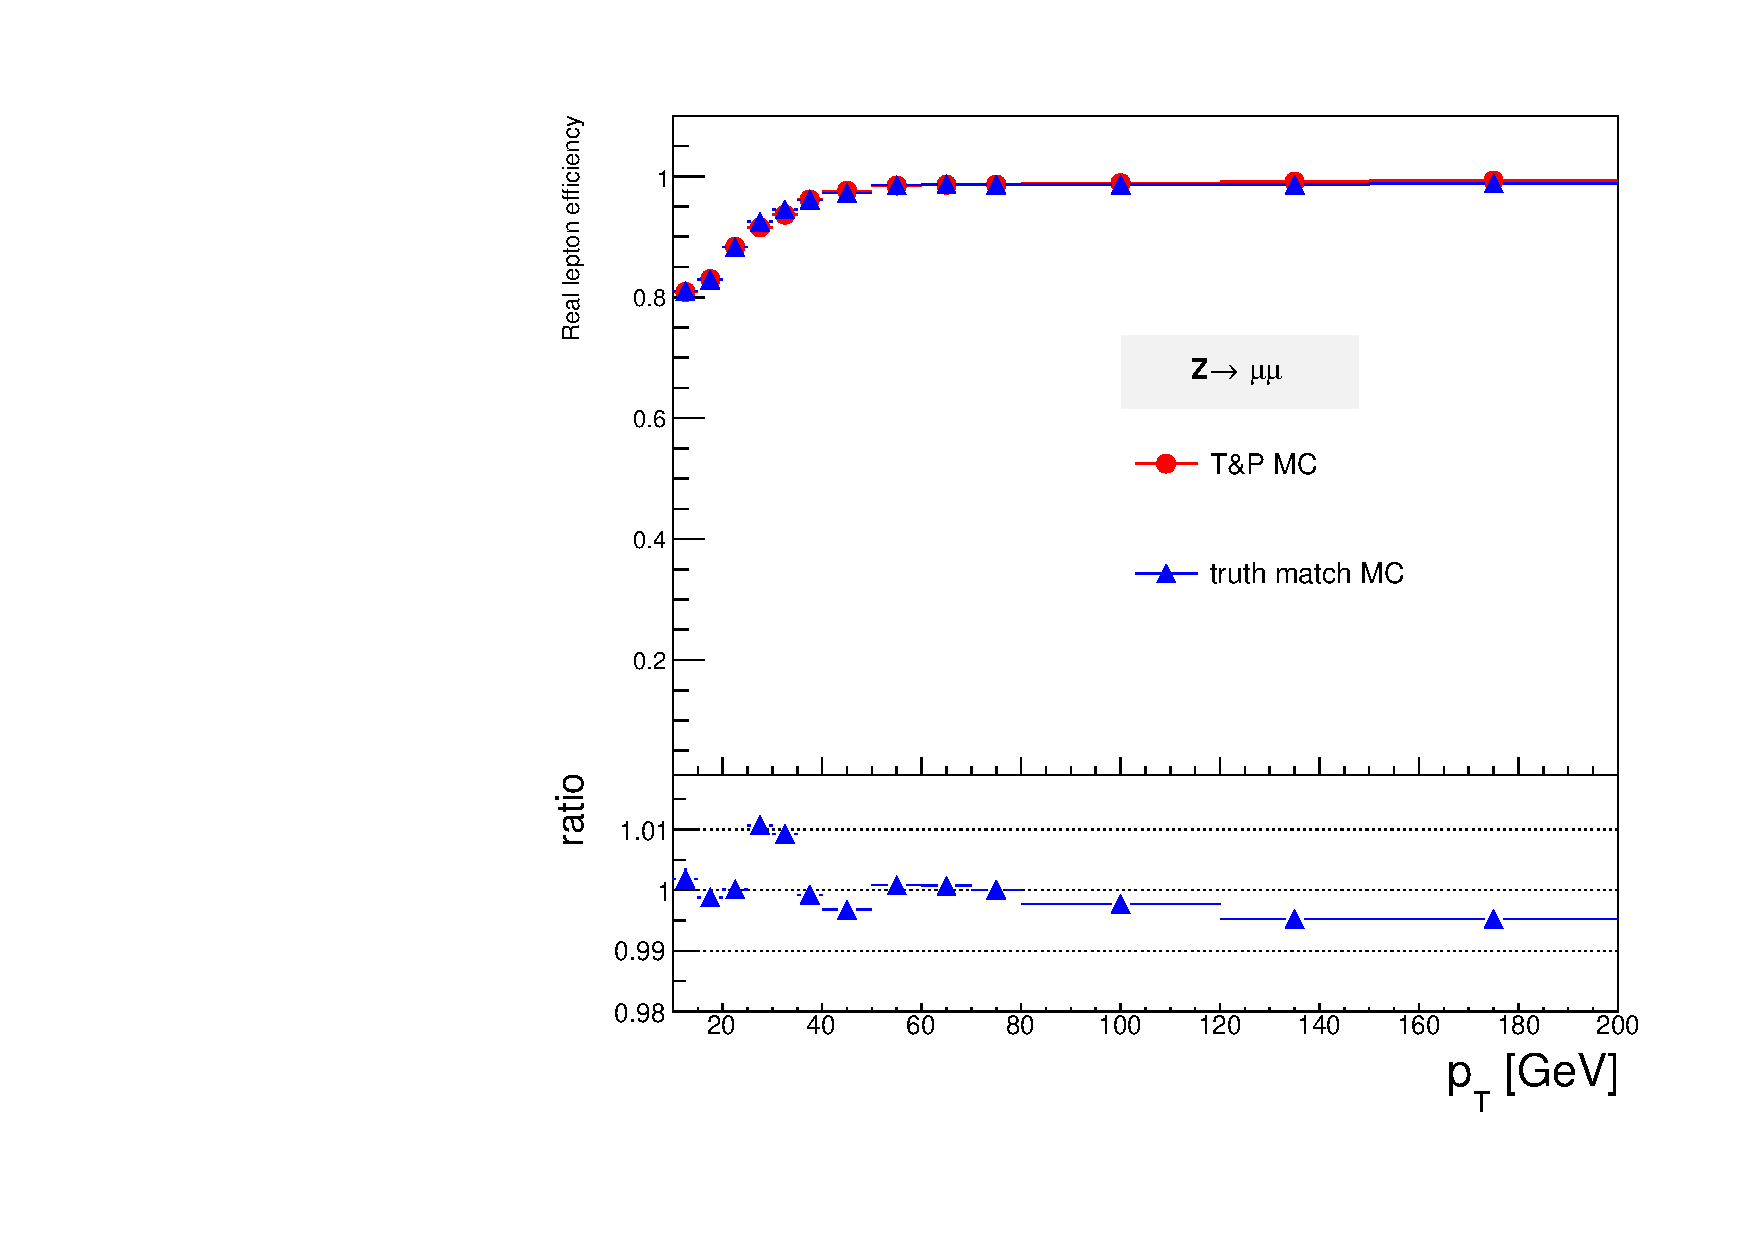
\includegraphics[width=0.33\textwidth]{Compare_TandP_truth_match_muon_pt.pdf}
    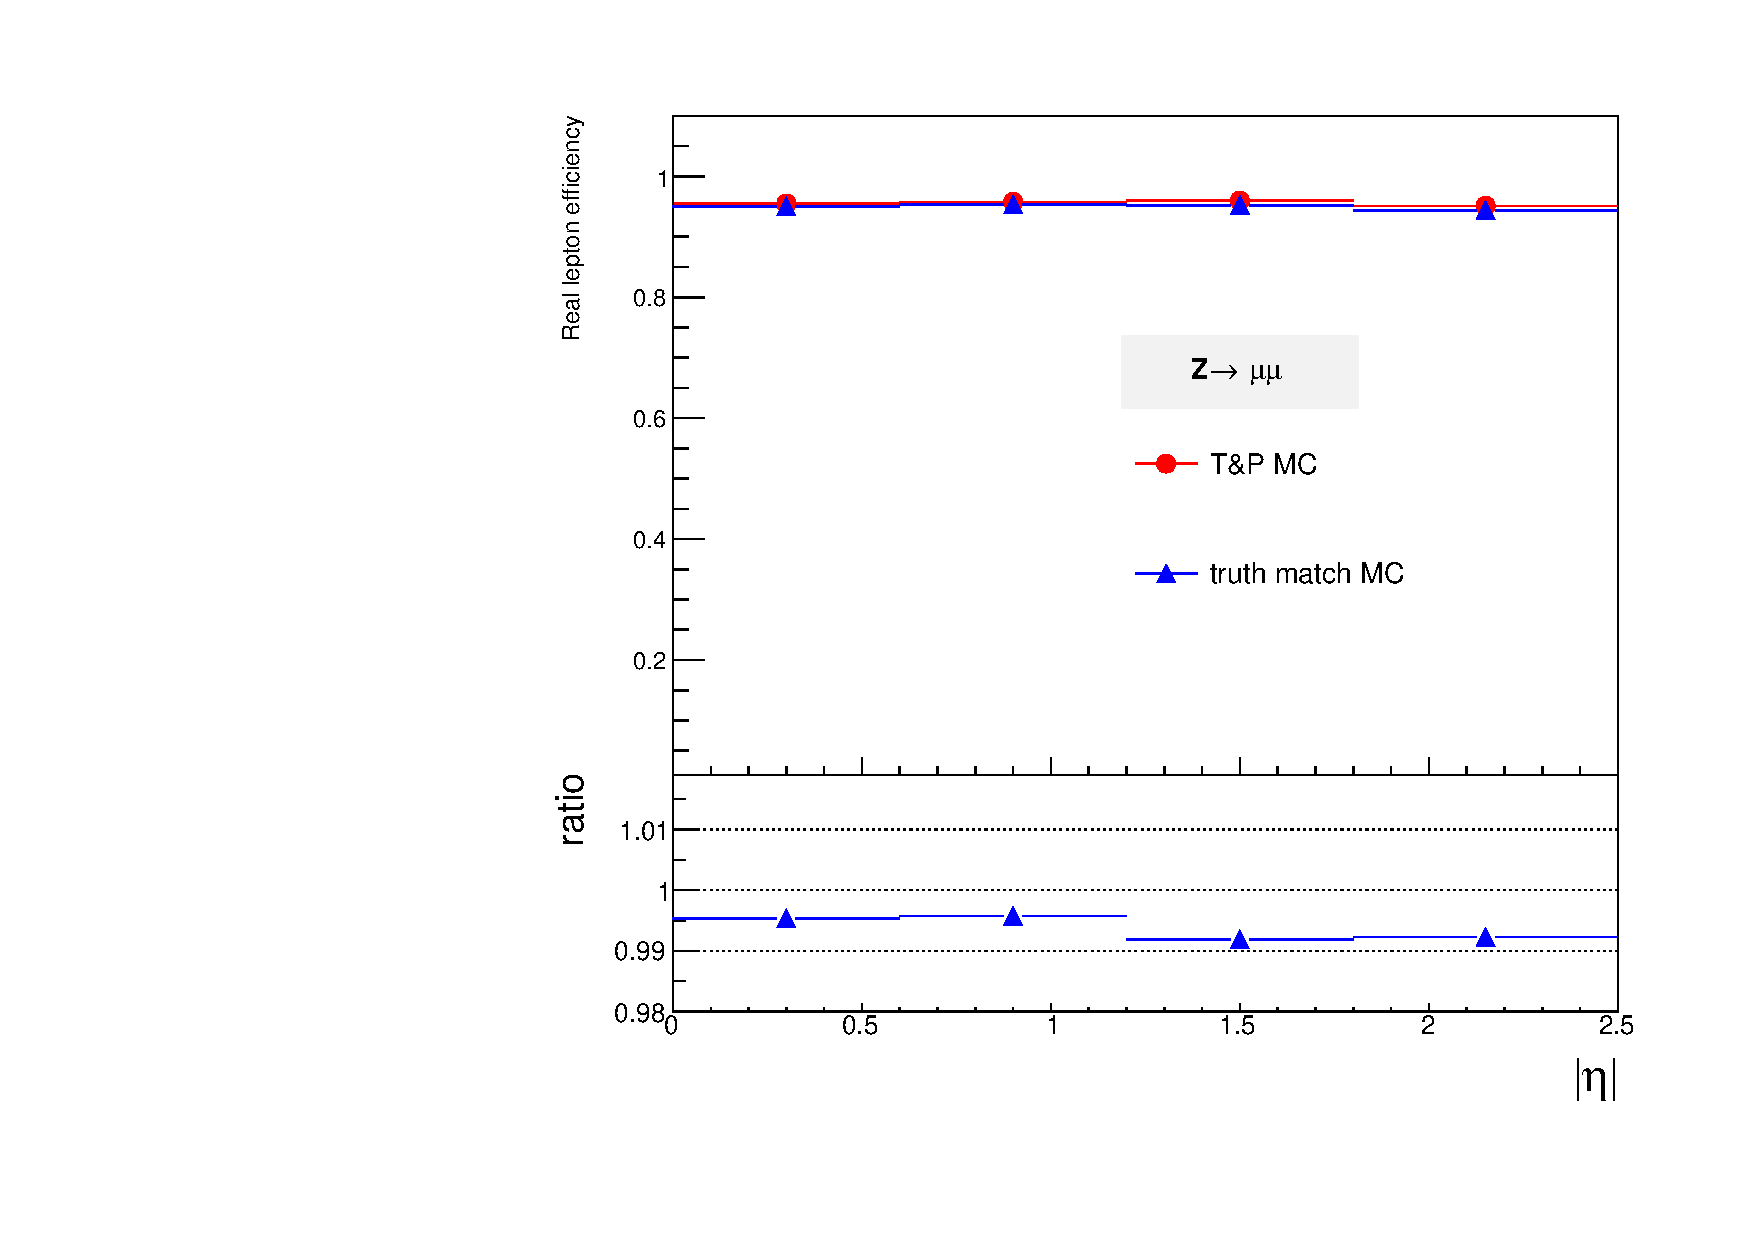
\includegraphics[width=0.33\textwidth]{Compare_TandP_truth_match_muon_eta.pdf}
    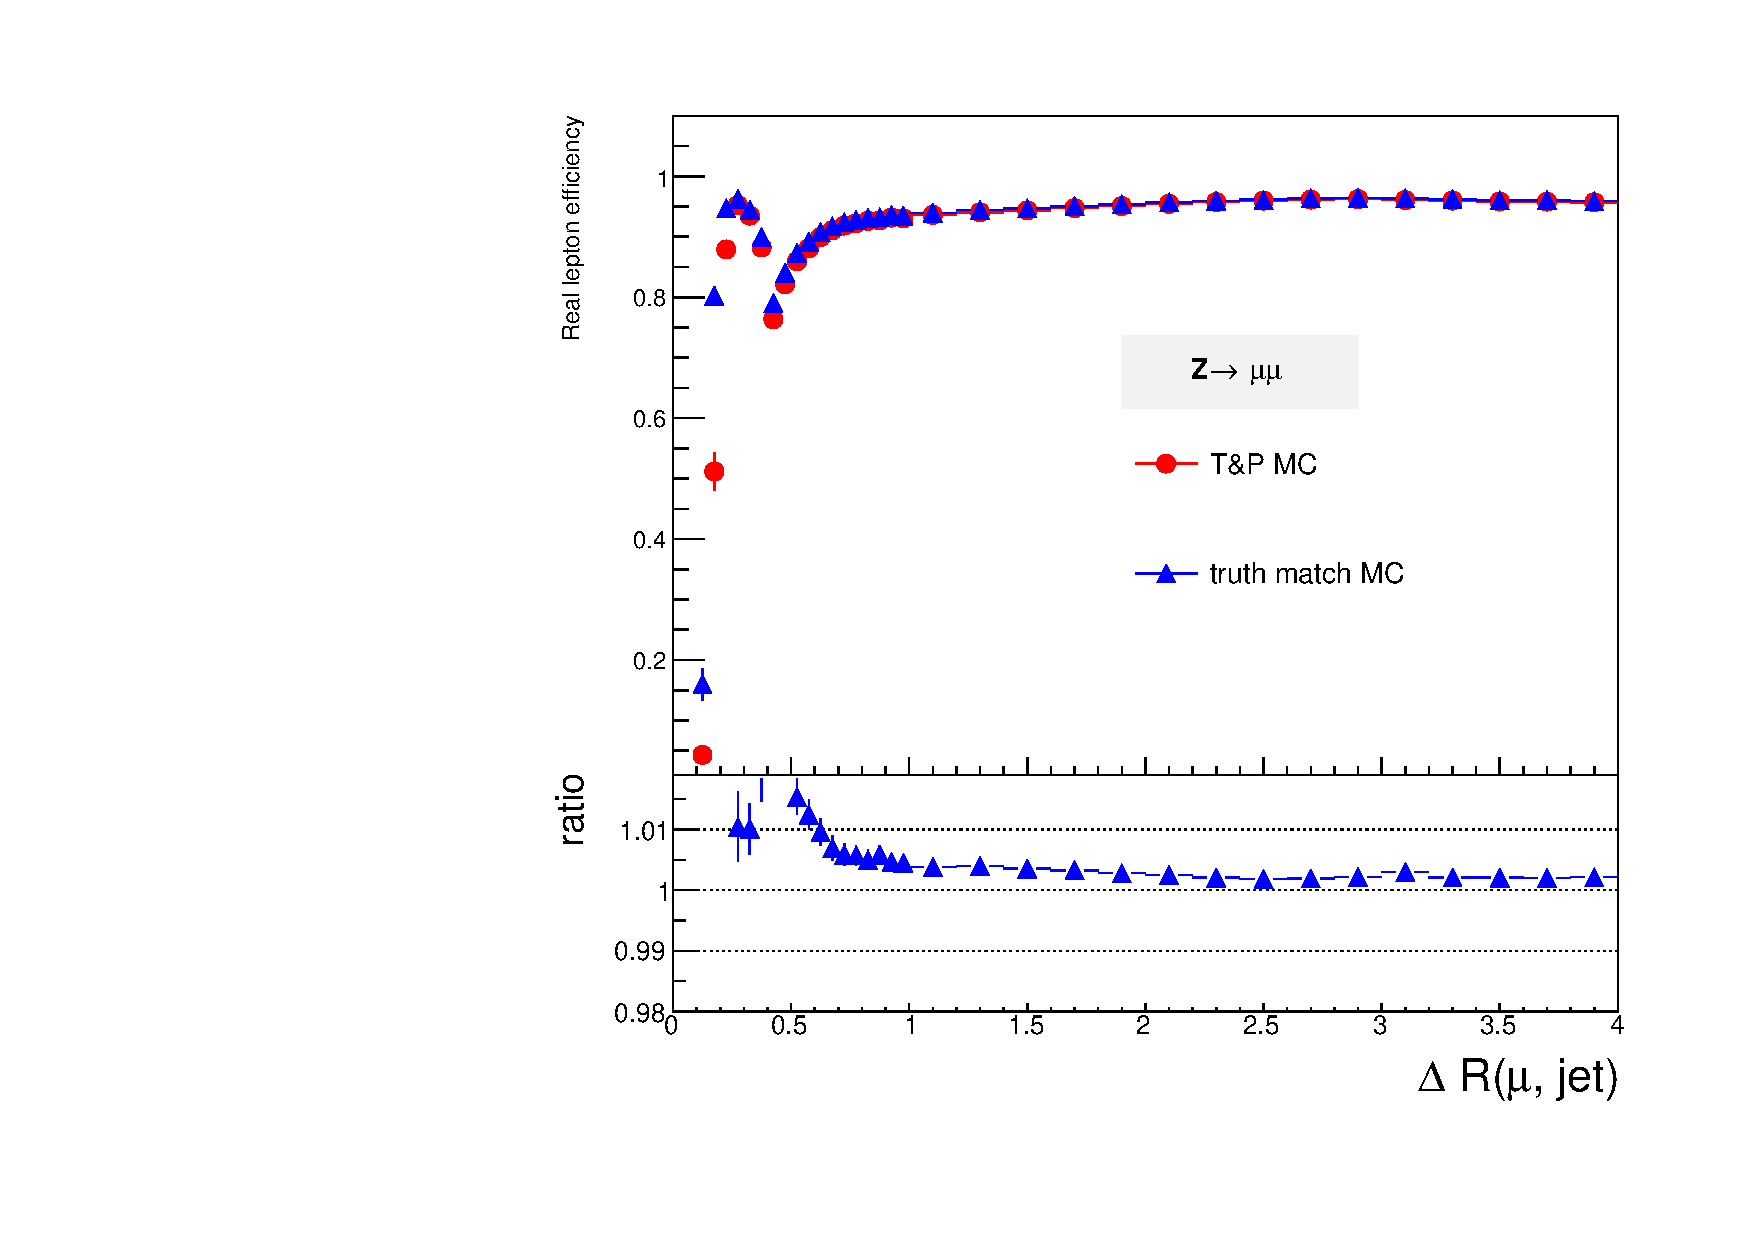
\includegraphics[width=0.33\textwidth]{Compare_TandP_truth_match_muon_dRjet.pdf}
    \caption{The real lepton efficiencies computed by $Z$ tag-and-probe method (red dots) and truth matching (blue triangles).
    The electron cases are on the top row and muon cases are at the bottom row.
    The three columns from the left to the right are the real lepton efficiencies as a function \pt, $|\eta|$, and $\Delta R(\ell, \mathrm{jet})$, respectively.
    The lower pads show the ratio with respect to the $Z$ tag-and-probe method.}
    \label{fig:app_RLE_TandP_truth_match_comparisons}
\end{figure}
%
The associated uncertainties are statistical uncertainties only.
For the real electron efficiencies, the largest difference is $\sim$7\% in low \pt and no differences can be seen when $\pt > 50$~{\GeV}; the largest difference is $\sim$3\% in ; the larger differences in $\Delta R(e, \mathrm{jet})$ exist when $\Delta R(e, \mathrm{jet}) < 0.4$.
Because the overlap removal has been applied on the baseline electrons, the $\Delta R(e, \mathrm{jet}) < 0.4$ region lacks statistics.
For the real muon efficiencies, the differences are less then 1\% for \pt and $|\eta|$.
However, the differences are larger for $\Delta R(\mu, \mathrm{jet}) < 0.4$ also because of the overlap removal.
The small differences between two methods indicate the robust of $Z$ tag-and-probe method and the differences may be considered as the systematic uncertainties.

%%%
%%%
%%%

\subsection{Data-to-MC comparisons}
\label{subsec:RLE_data_to_mc_comparisons}
The real lepton efficiencies calculating by data and $Z\to \ell\ell$ MC samples are compared.
All 2015 and 2016 data are considered corresponding to an integrated luminosity of 36.5 \ifb.
All the lepton scale factors are applied on the MC samples and the simulation is reweighted to the pile-up observed in data.
Figure~\ref{fig:app_RLE_real_efficiency_pt_eta_dRjet} shows the real efficiencies as a function of \pt, $|\eta|$ and $\Delta R(\ell, \mathrm{jet})$ using data and $Z\to \ell \ell$ MC samples, respectively.
The associated uncertainties are statistical uncertainties only.























  computed using the $Z$ tag-and-probe method in  are compared to those using the simulated  processes.

All the MC  provided by the CP group are applied and the simulation is reweighted to the pile-up observed in the data.
%Besides, an additional truth match is added for the MC lepton selection.

The associated uncertainties correspond to the statistical uncertainties only.
A reasonable data to MC agreement is observed except the low $\Delta R(\ell, jet)$ region because of lacking statistics.
The real electron efficiencies as a function of $|\eta|$ computed using the $Z\to ee$ MC are slightly lower than the one computed using data.
The differences come from the efficiencies drop of $Z\to ee$ MC in the $40<\pt<\SI{50}{GeV}$. 

\begin{figure}[htbp]
    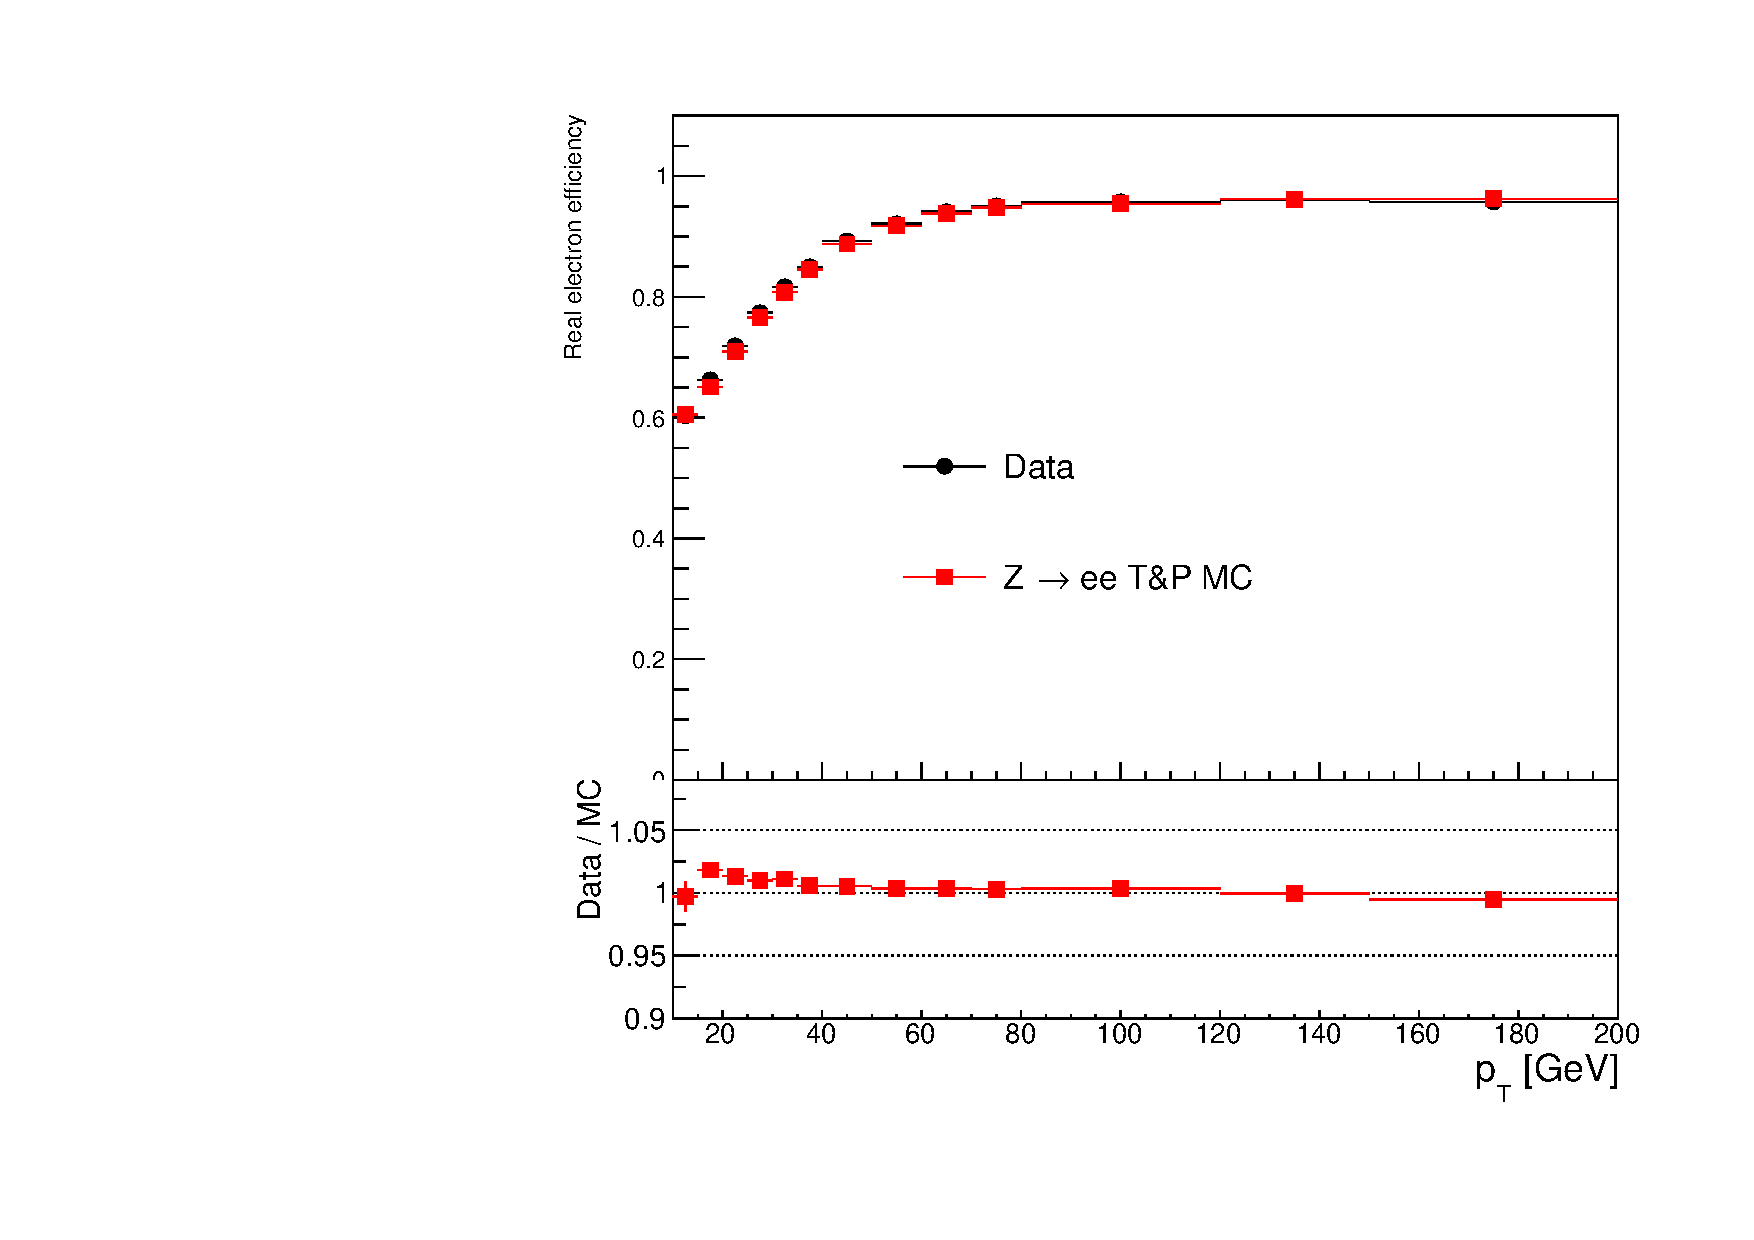
\includegraphics[width=0.33\textwidth]{real_efficiency_ratio_plot_electron_pt.pdf}
    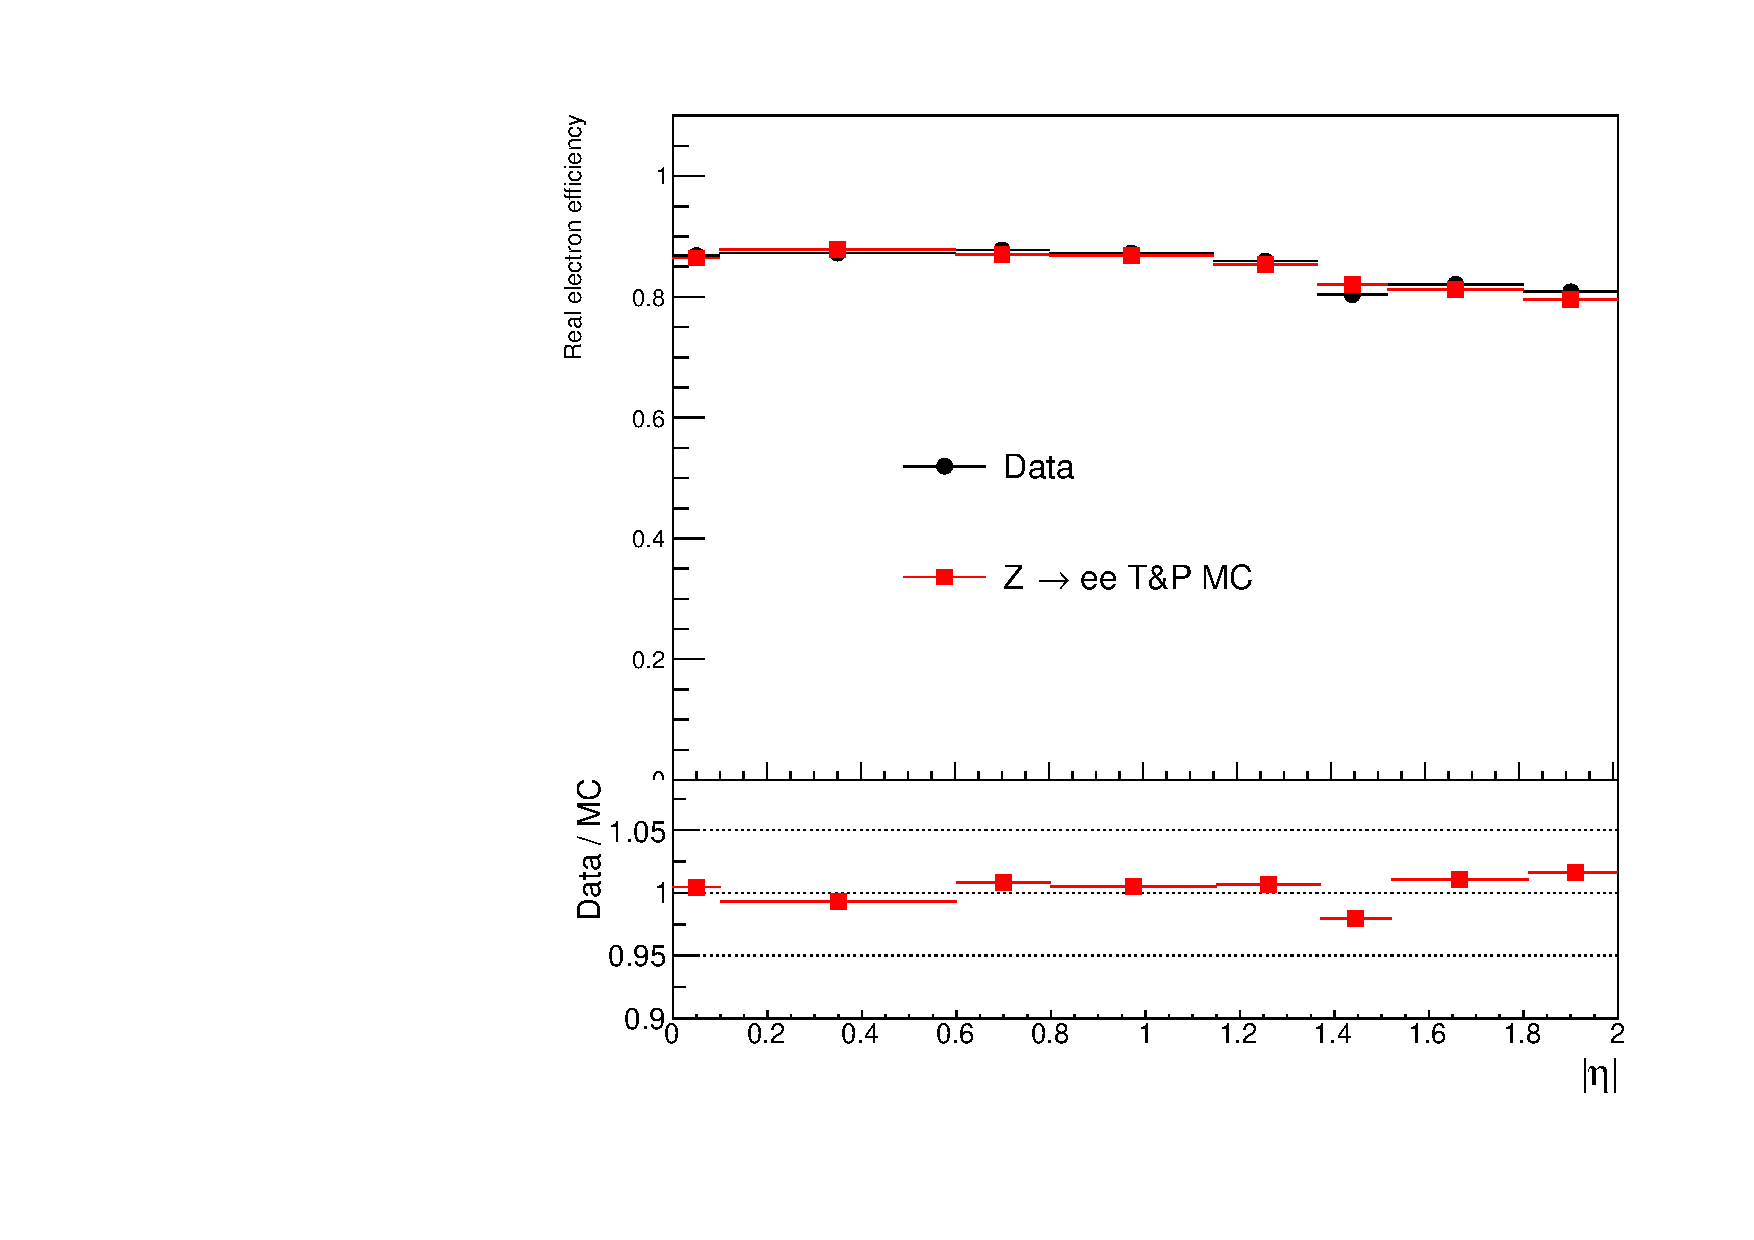
\includegraphics[width=0.33\textwidth]{real_efficiency_ratio_plot_electron_eta.pdf}
    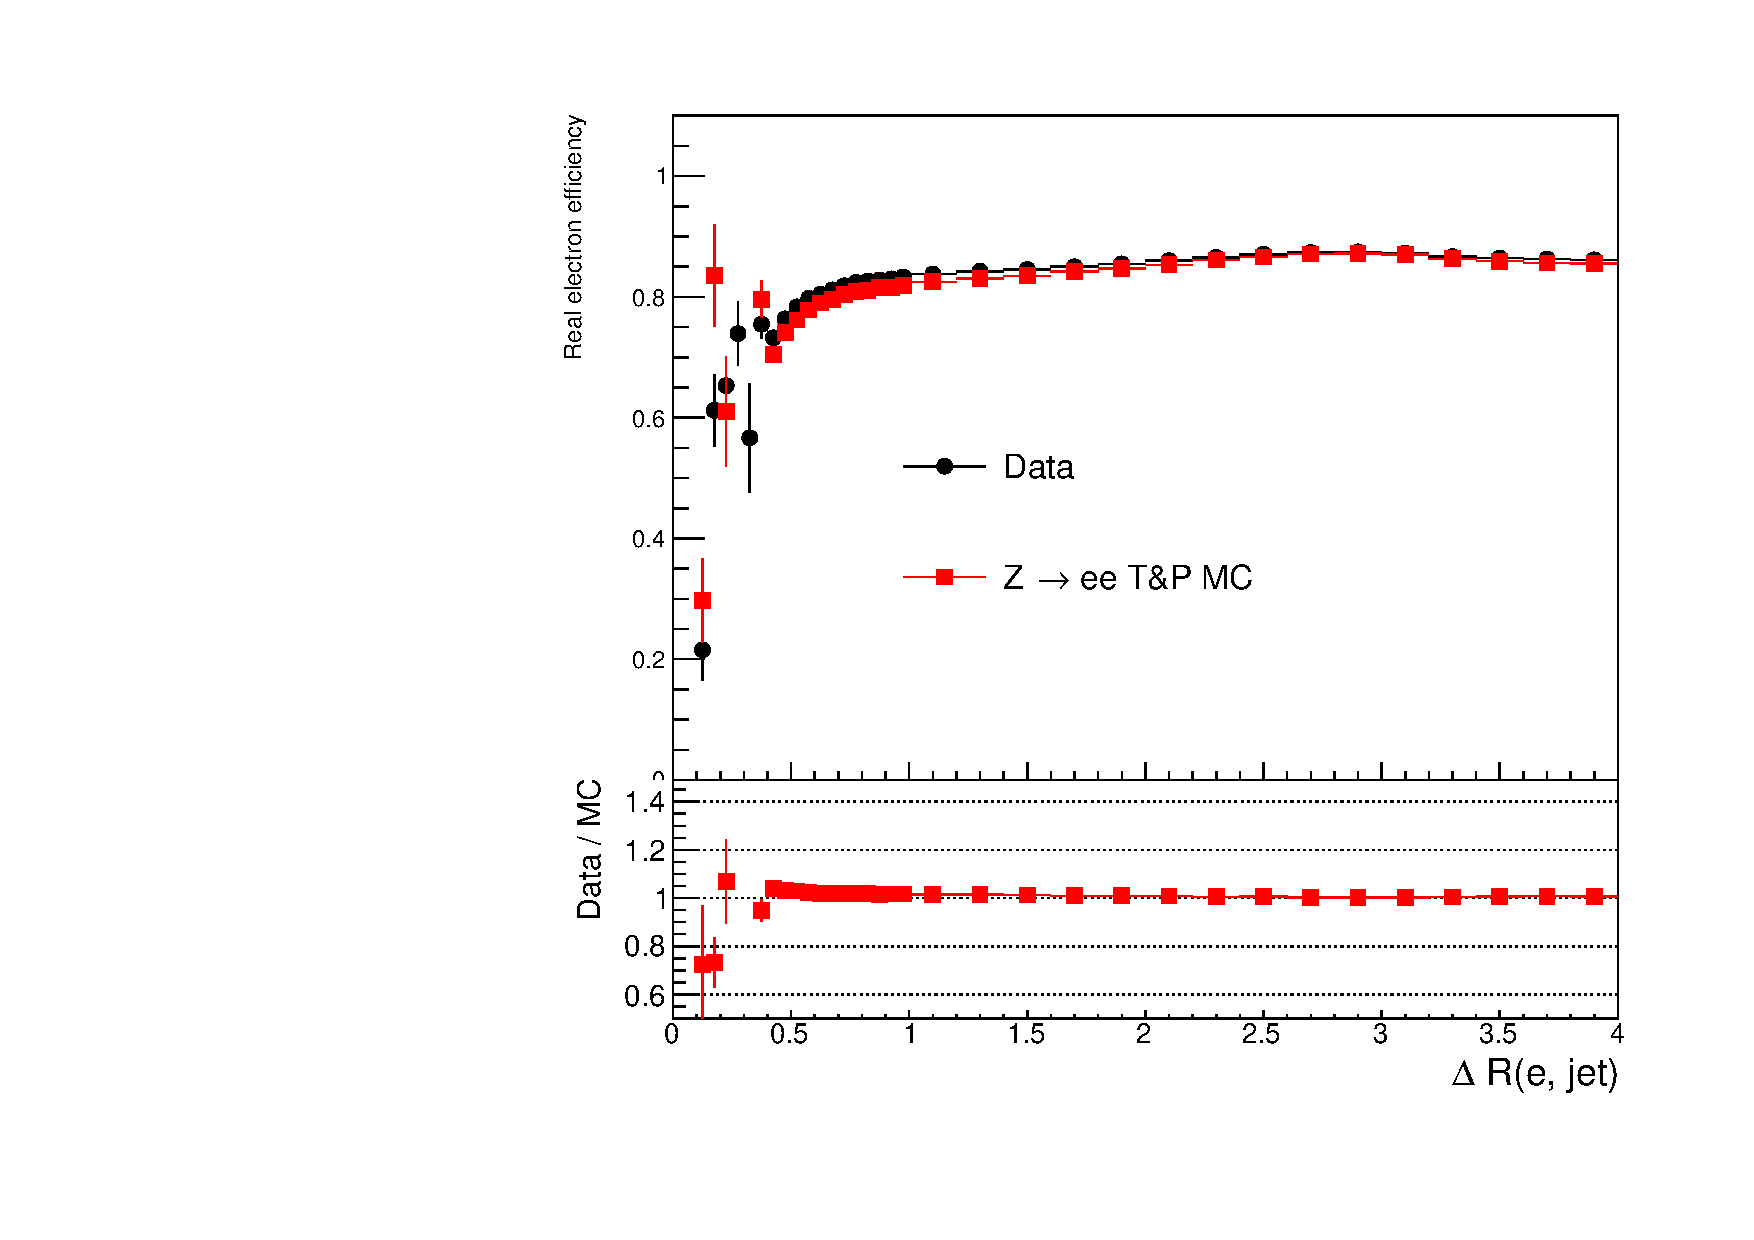
\includegraphics[width=0.33\textwidth]{real_efficiency_ratio_plot_electron_dRjet.pdf}\\
    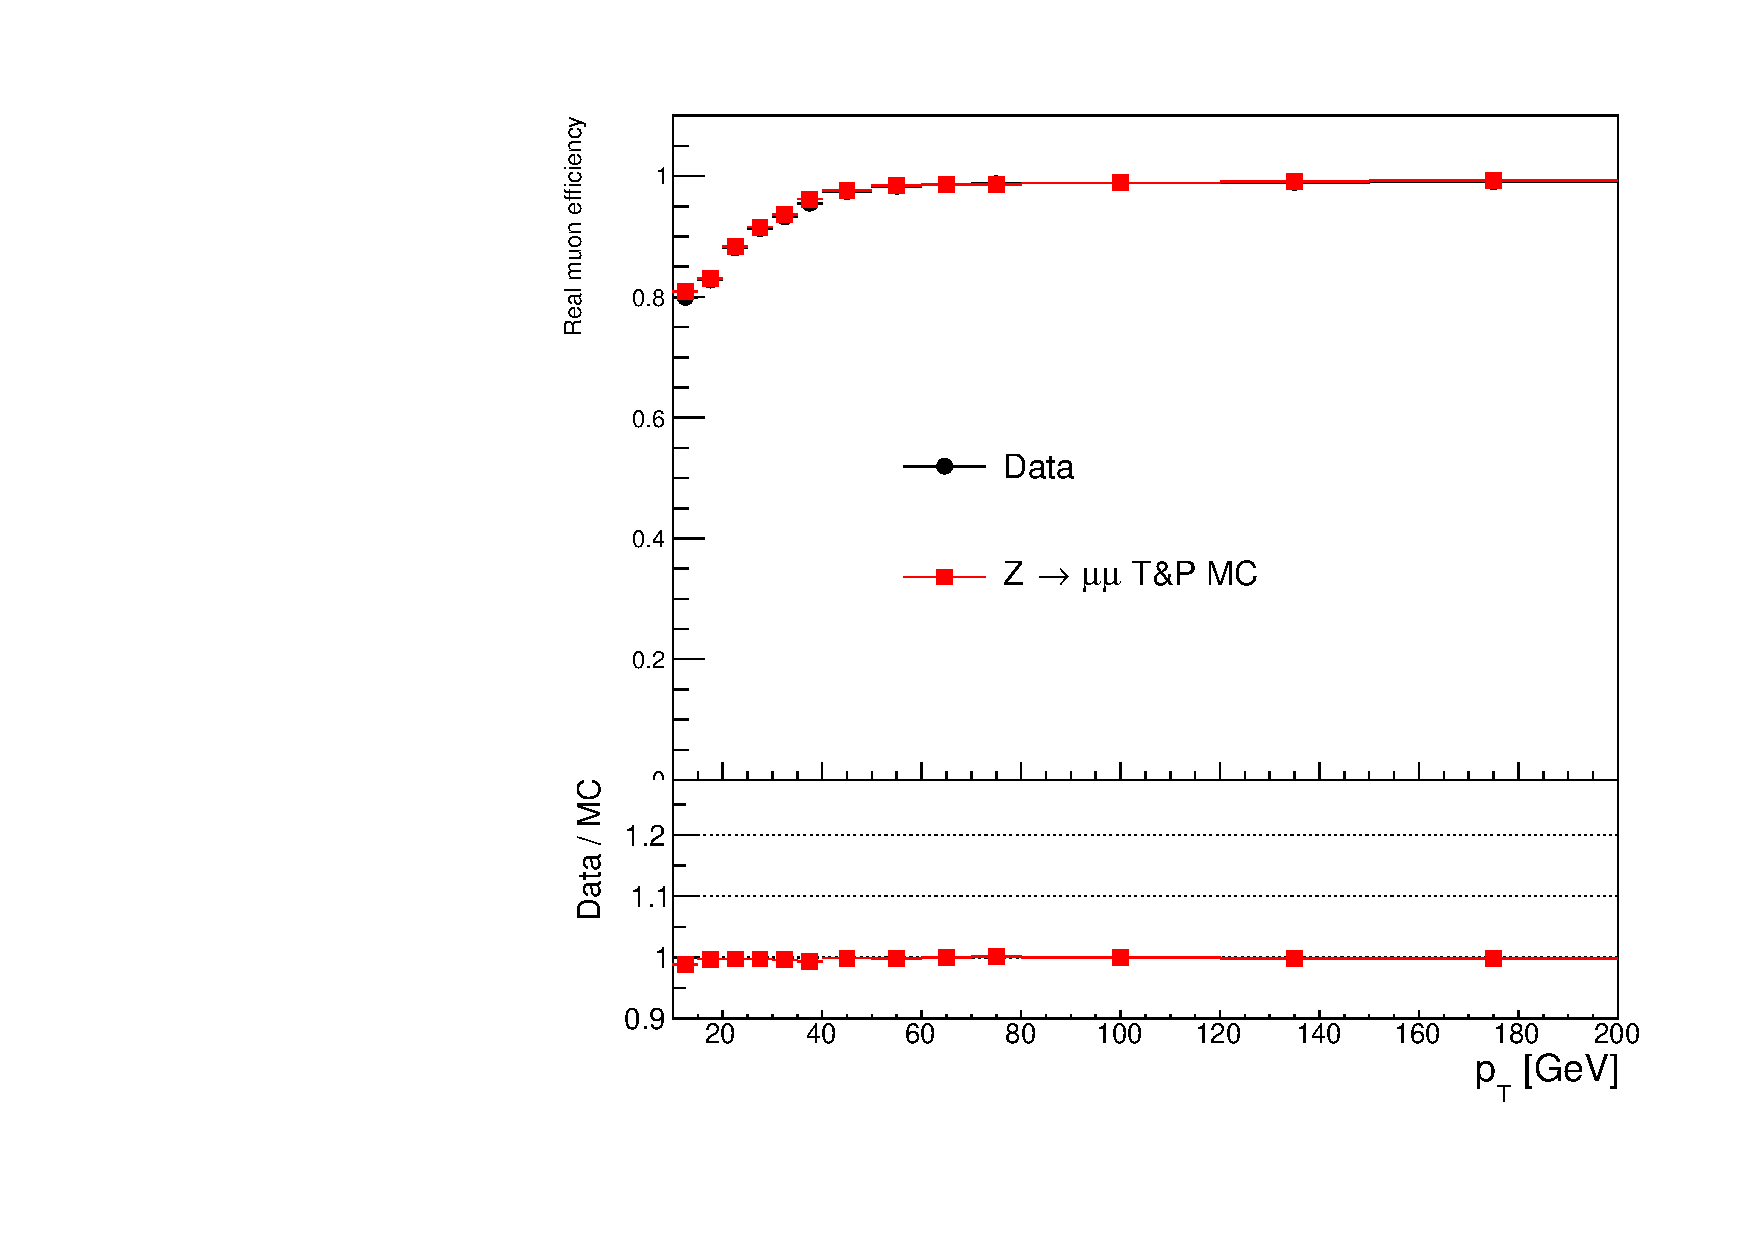
\includegraphics[width=0.33\textwidth]{real_efficiency_ratio_plot_muon_pt.pdf}
    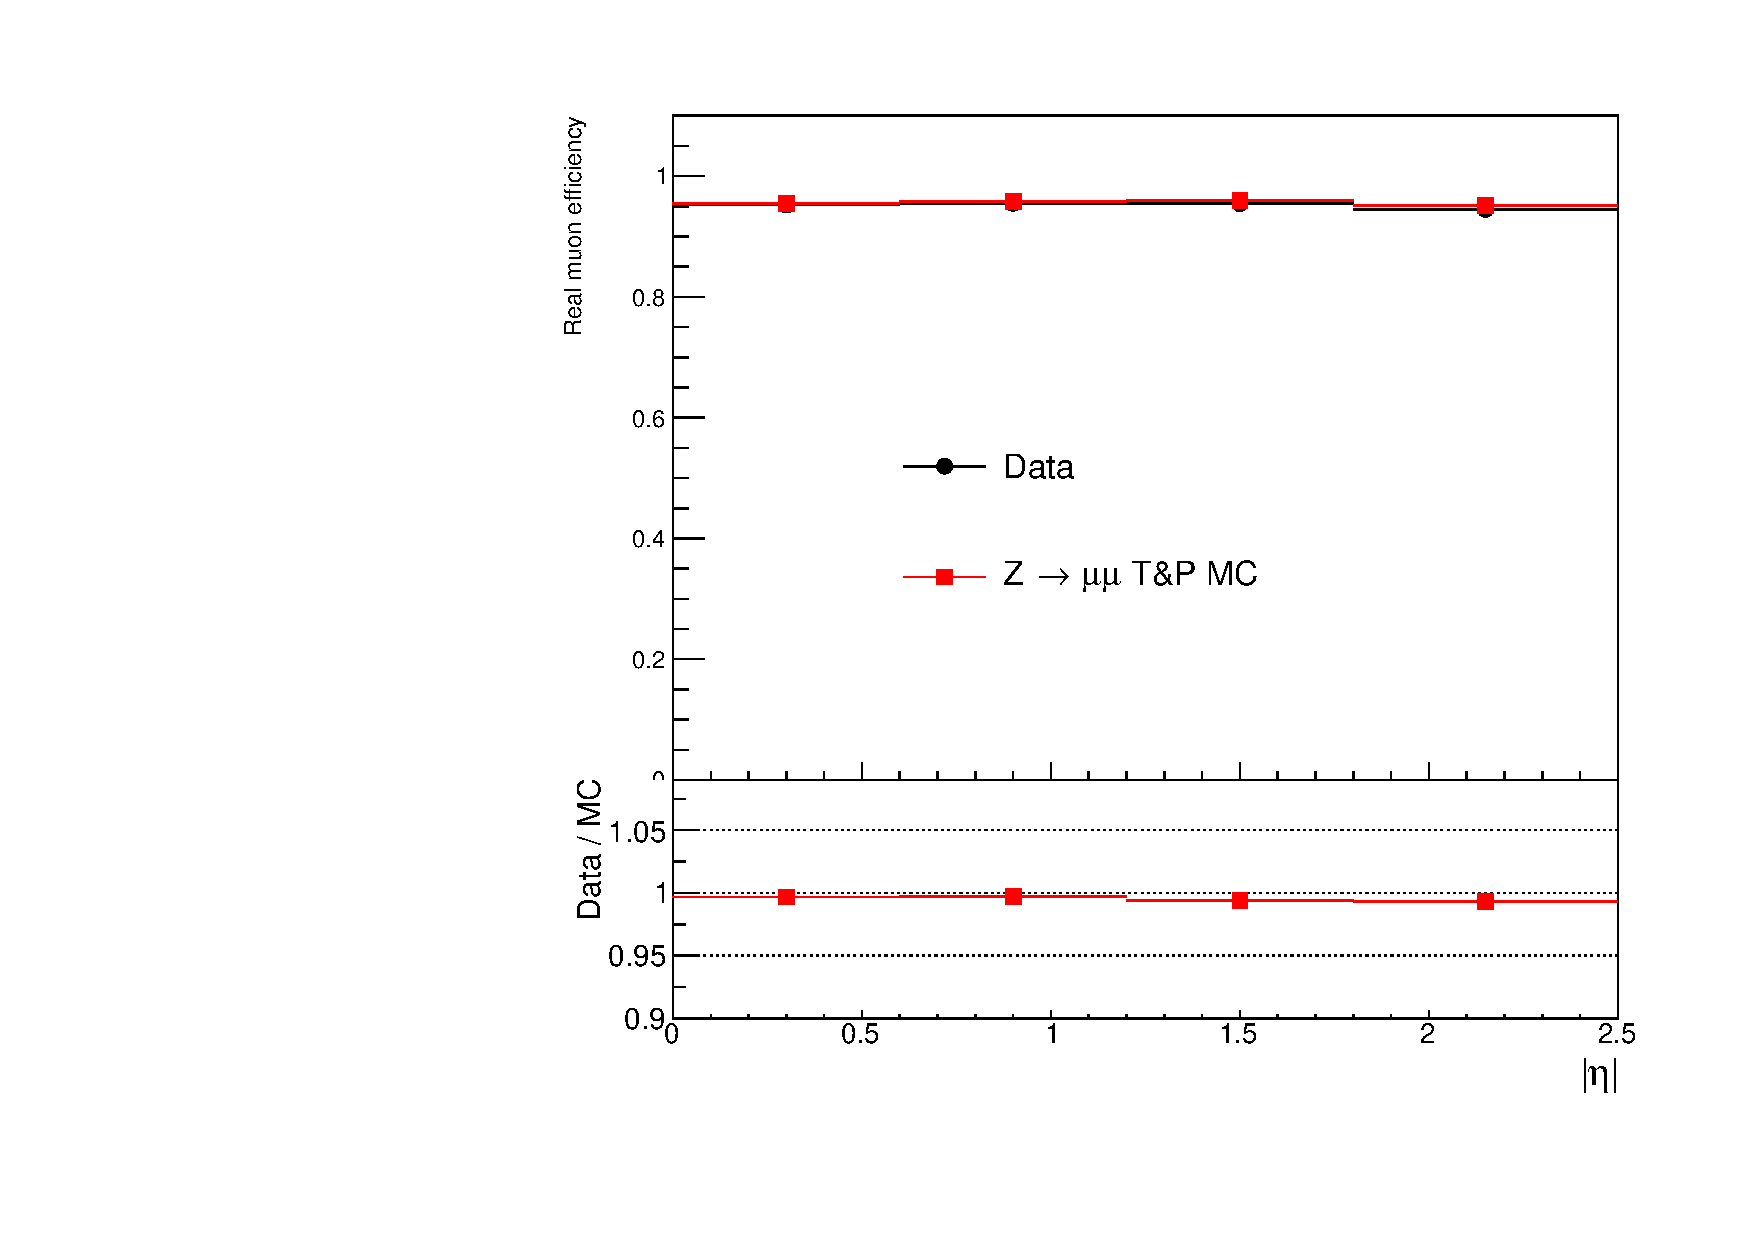
\includegraphics[width=0.33\textwidth]{real_efficiency_ratio_plot_muon_eta.pdf}
    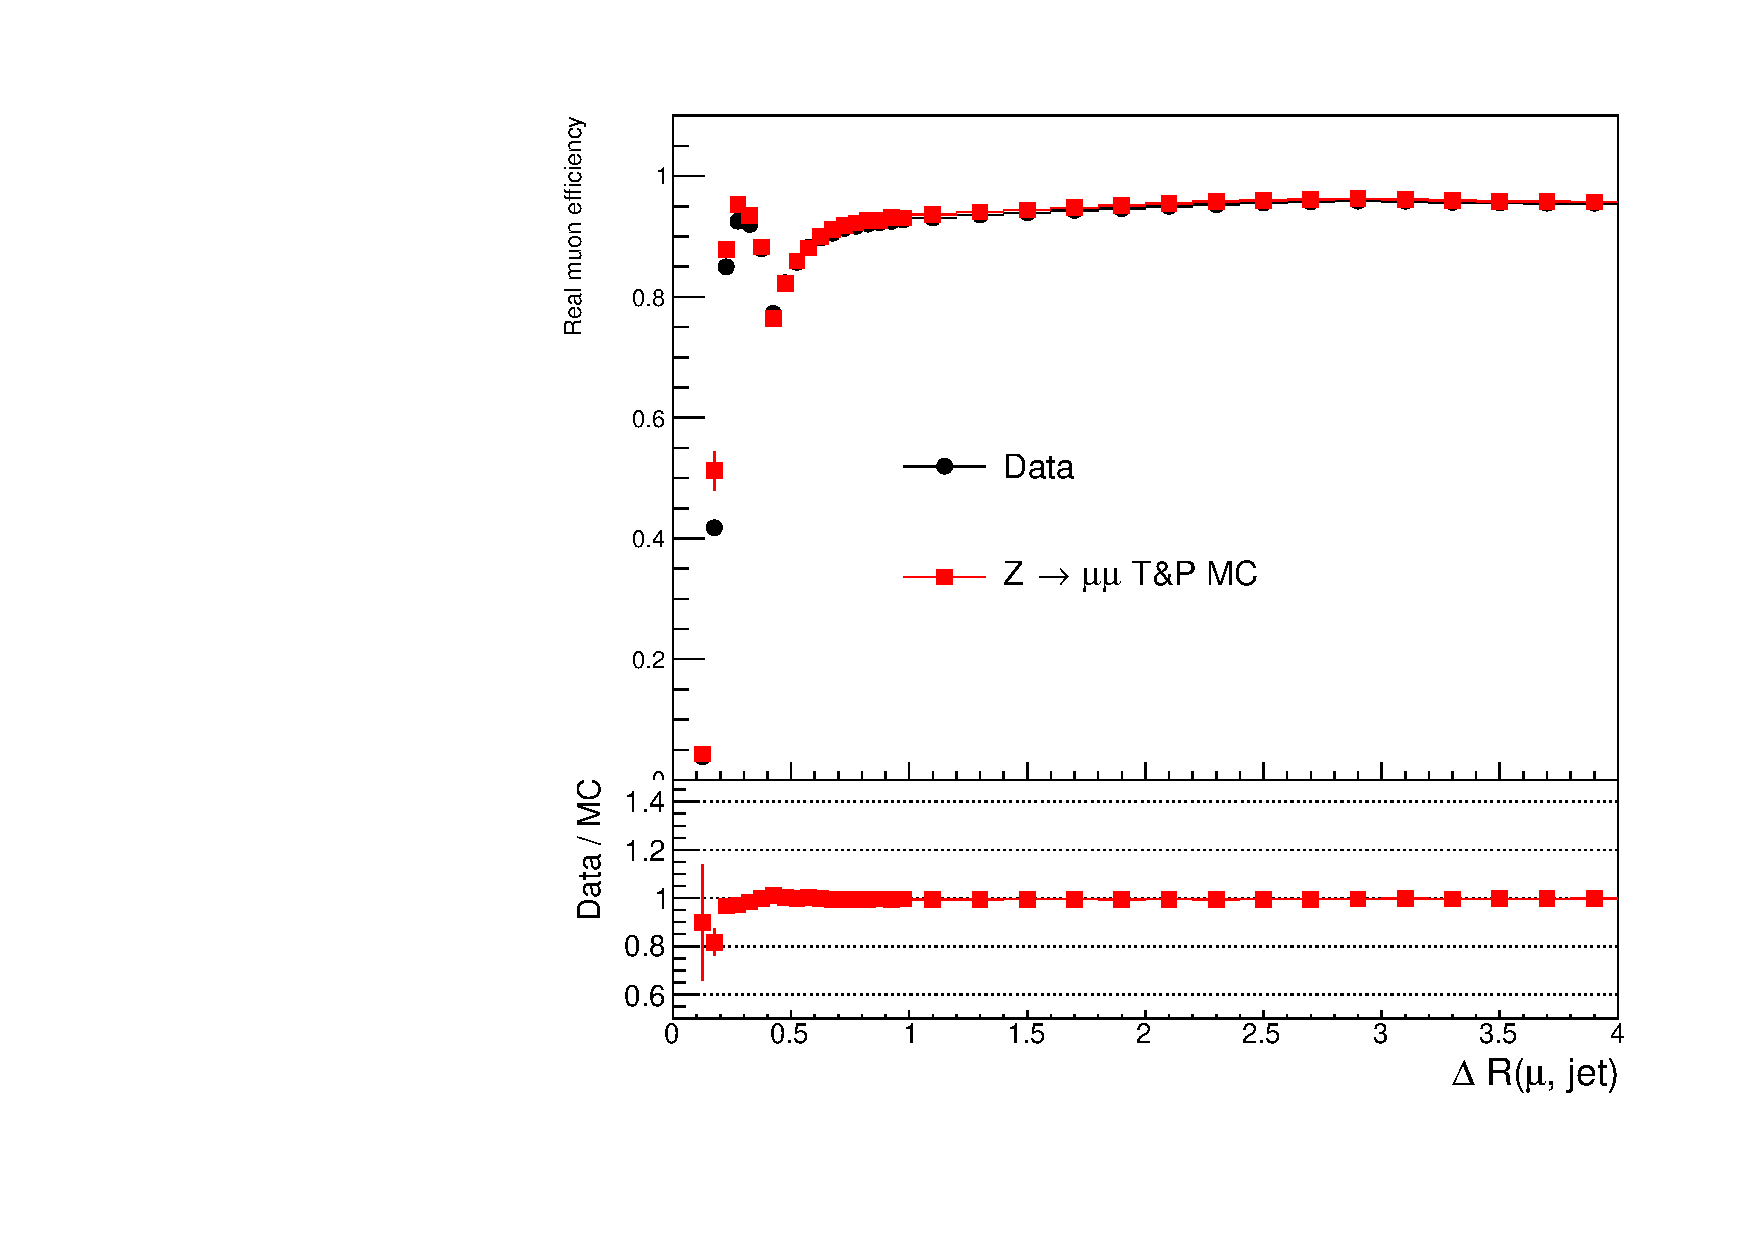
\includegraphics[width=0.33\textwidth]{real_efficiency_ratio_plot_muon_dRjet.pdf}
    \caption{The real lepton efficiencies as a function of $\pt$, $|\eta|$ and $\Delta R(\ell, jet)$ measured on data and MC using the $Z$ tag-and-probe method.
    The plots on the top row correspond to the real electron efficiencies and the plots on the bottown row correspond to the real muon efficiencies.
    The 2015 + 2016 data are denoted by the black dots, the $Z\to\ell\ell$ MC are shown using red squares and are reweighted to the data pile-up.
    The uncertainties shown in the plots are corresponding to the statistical uncertainties only.
    Some differences between data and $Z\to \ell\ell$ MC can be seen in the low $\Delta R(\ell, jet)$ region.
    The binning used for the real electron efficiencies as a function of $\eta$ corresponds to the geometry of the electromagnetic calorimeter.}
    \label{fig:app_RLE_real_efficiency_pt_eta_dRjet}
\end{figure}



\subsubsection{Real lepton efficiency versus pileup}
\label{subsubsec:RLE_vs_pileup}
 
The relations between the real lepton efficiencies and the pileup are also studied.
The efficiencies calculated using 2015 + 2016 data are compared with those obtained using $Z$ tag-and-probe method and truth matching MC samples.
The \ttbar and $\tilde{g}\to\ttbar\tilde{\chi^{0}_{1}}$ MC samples are also considered because we are interested in the behavior of the efficiencies with different event topologies.
Figure~\ref{fig:RLE_vs_pileup} shows the electron and muon real efficiencies as a function of the average interactions per crossing $<\mu>$.
The real electron efficiencies are about 92\% to 93\% at low $<\mu>$ and decrease when $<\mu>$ increase.
Comparing with the real lepton efficiencies calculated by data samples, the efficiencies computed using $\tilde{g}\to\ttbar\tilde{\chi^{0}_{1}}$ MC sample have lower efficiencies in both electron and muon cases.
But the real lepton efficiencies computed by the \ttbar have similar efficiencies with the data one in the electron case and have lower efficiencies in the muon case.
This is because the \ttbar MC has lower real muon efficiencies when $\pt<\SI{40}{GeV}$ with respect to data.
If we require a $\pt>\SI{40}{GeV}$ requirement on the probe leptons, then the real muon efficiencies for \ttbar MC agree with data.
The electron and muon real efficiencies as a function of $\pt$ compared with data and $Z\to\ell\ell$ are shown in Figure~\ref{fig:RLE_real_efficiency_ttbar_gtt}.
From which we notice the real lepton efficiencies of \ttbar process is lower than the data one when $\pt<\SI{40}{GeV}$ and the $\tilde{g}\to\ttbar\tilde{\chi^{0}_{1}}$ process has lower real lepton efficiencies in both electron and muon cases.

\begin{figure}[htbp]
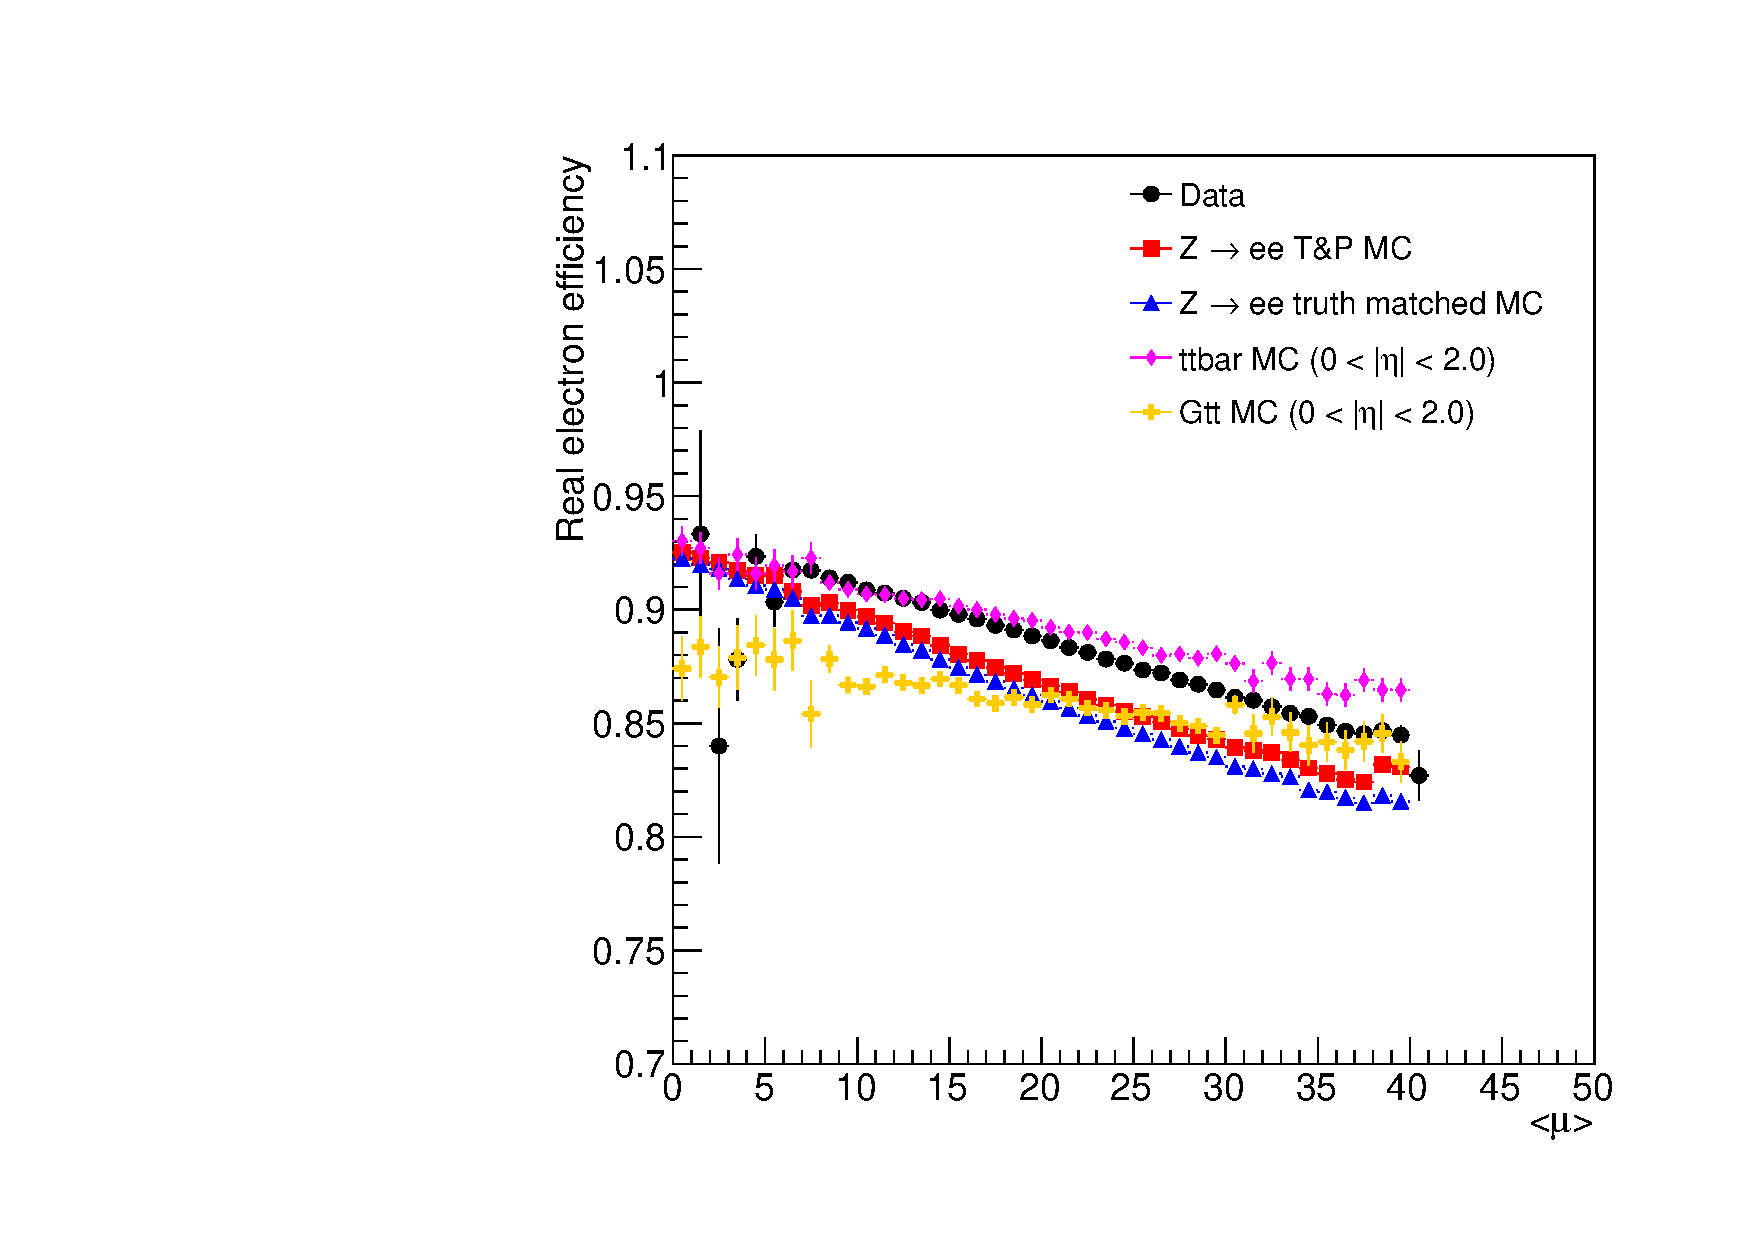
\includegraphics[width=0.48\textwidth]{real_efficiency_vs_AvgMu_elec.pdf}
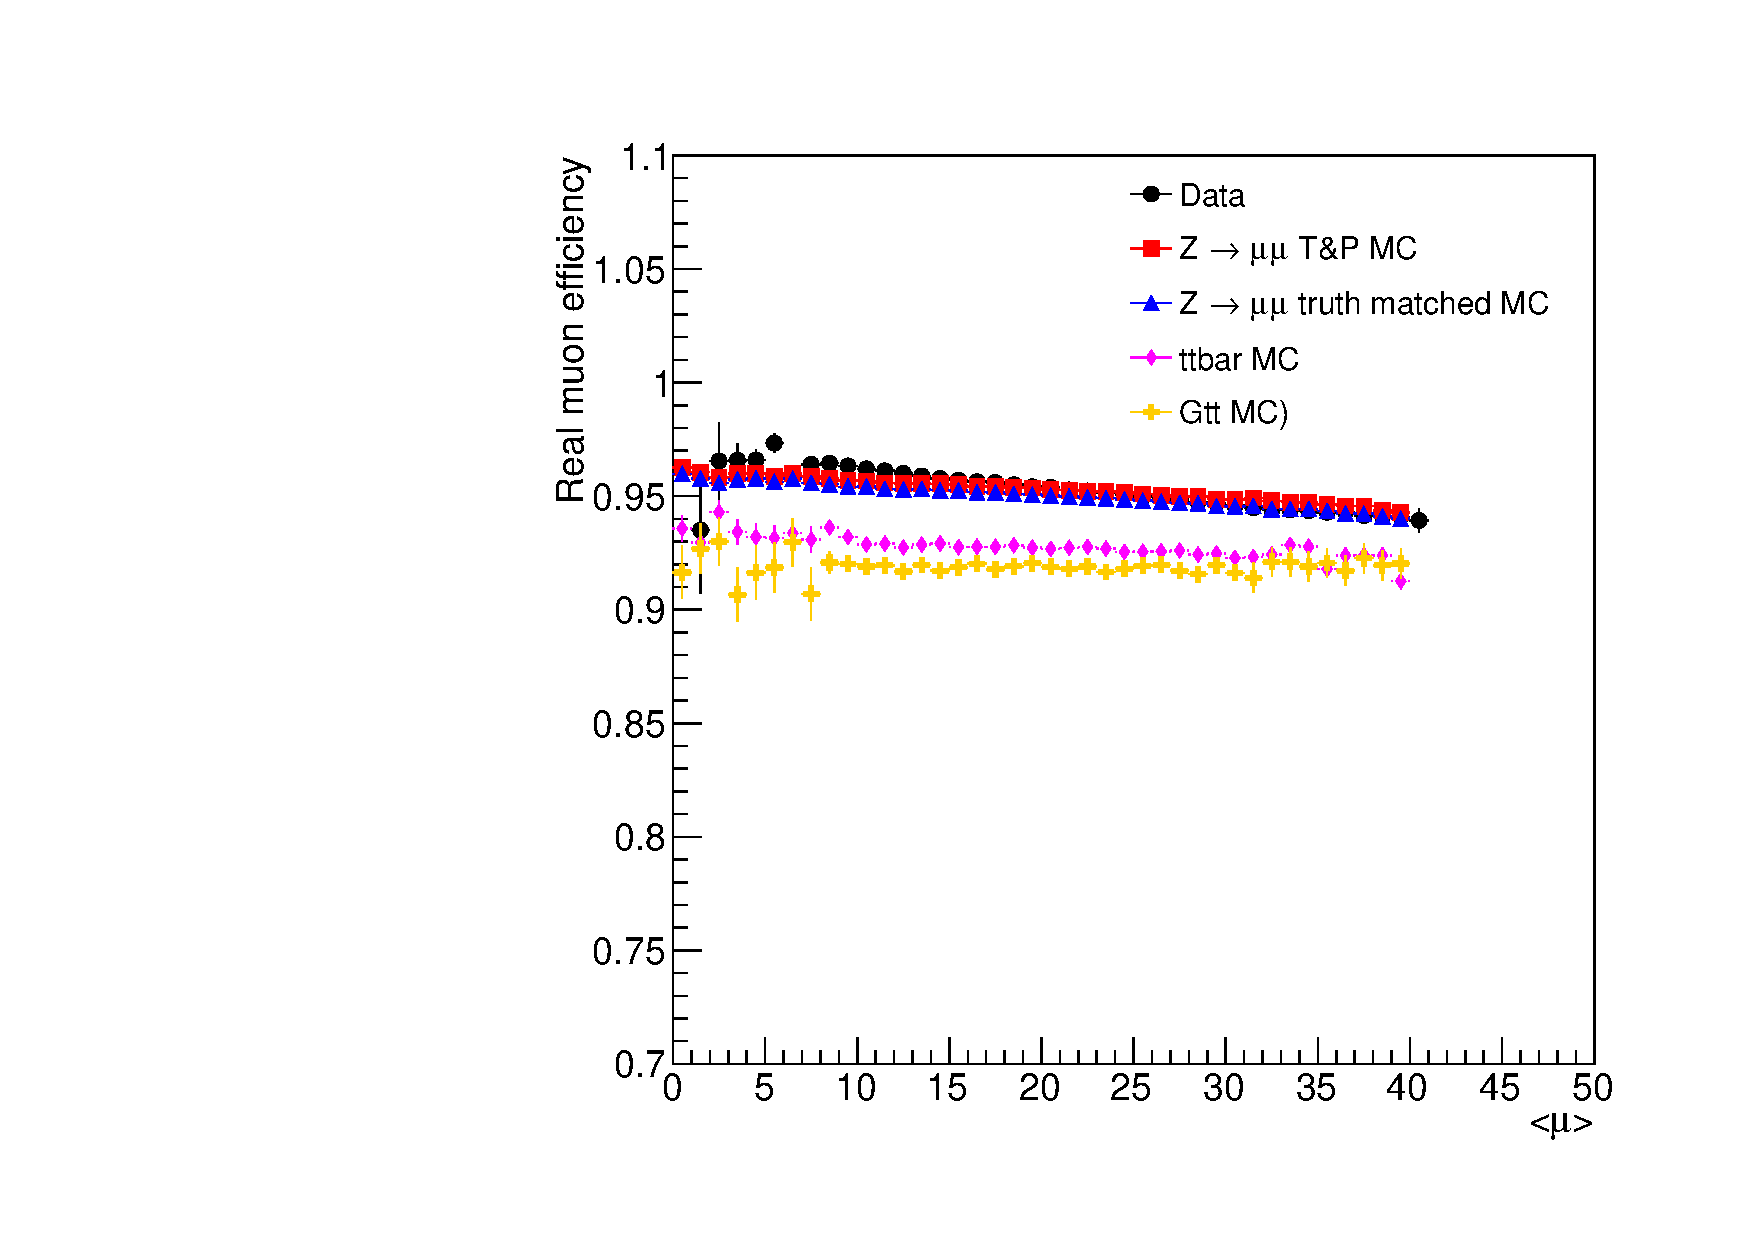
\includegraphics[width=0.48\textwidth]{real_efficiency_vs_AvgMu_muon.pdf}
\caption{
The real lepton efficiencies as a function of the average interactions per crossing $<\mu>$.
The data is shown as black dots and $Z\to \ell\ell$ tag-and-probe and truth matching are in red squares and blue triangles, respectively.
The real lepton efficiencies calculated using \ttbar and $\tilde{g}\to\ttbar\tilde{\chi^{0}_{1}}$ MC are also shown in magenta diamonds and yellow crosses.
And they show the real lepton efficiencies with different event topoloties.
The $|\eta|<2$ requirement has been applied on the \ttbar and $\tilde{g}\to\ttbar\tilde{\chi^{0}_{1}}$ MC samples for the electron case.
}
\label{fig:RLE_vs_pileup}
\end{figure}

\begin{figure}[htbp]
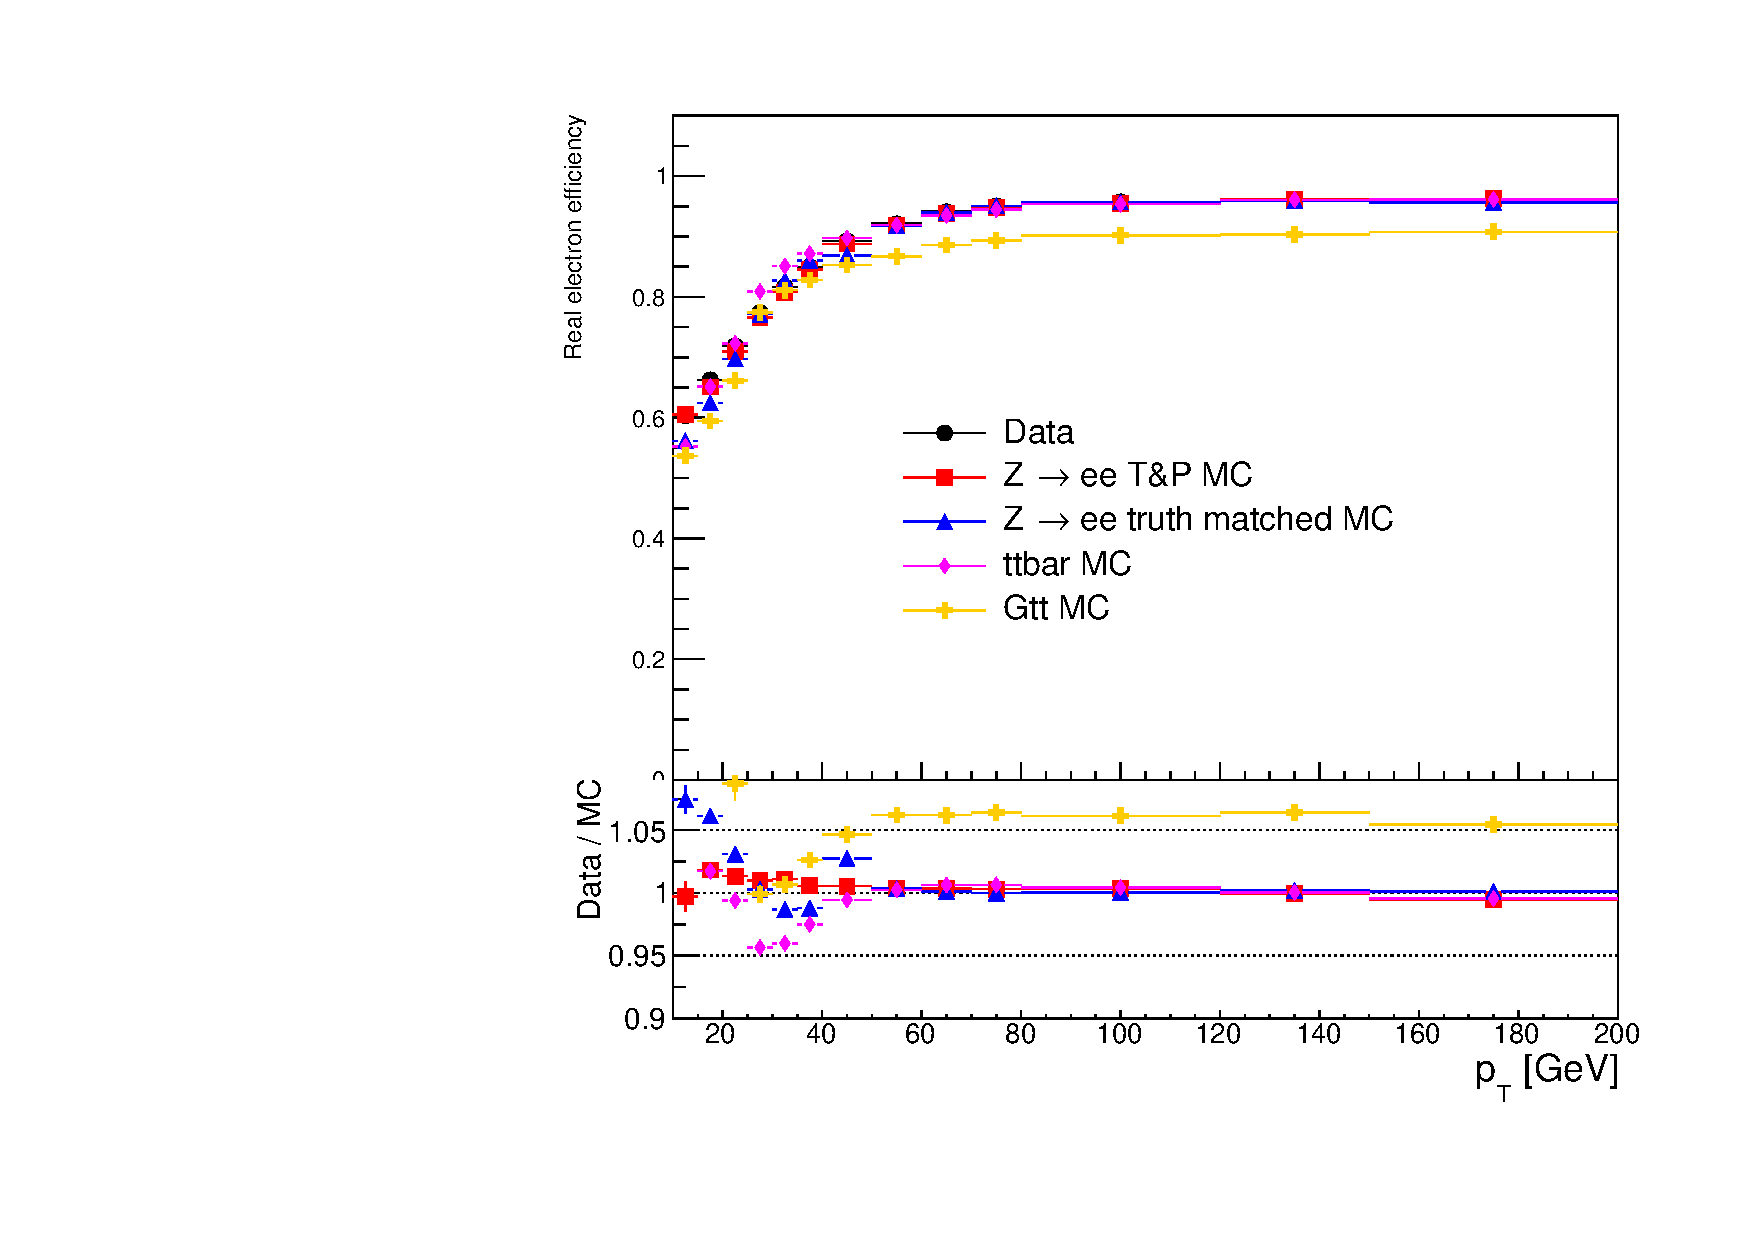
\includegraphics[width=0.48\textwidth]{real_efficiency_ratio_plot_electron_pt_ttbar_gtt.pdf}
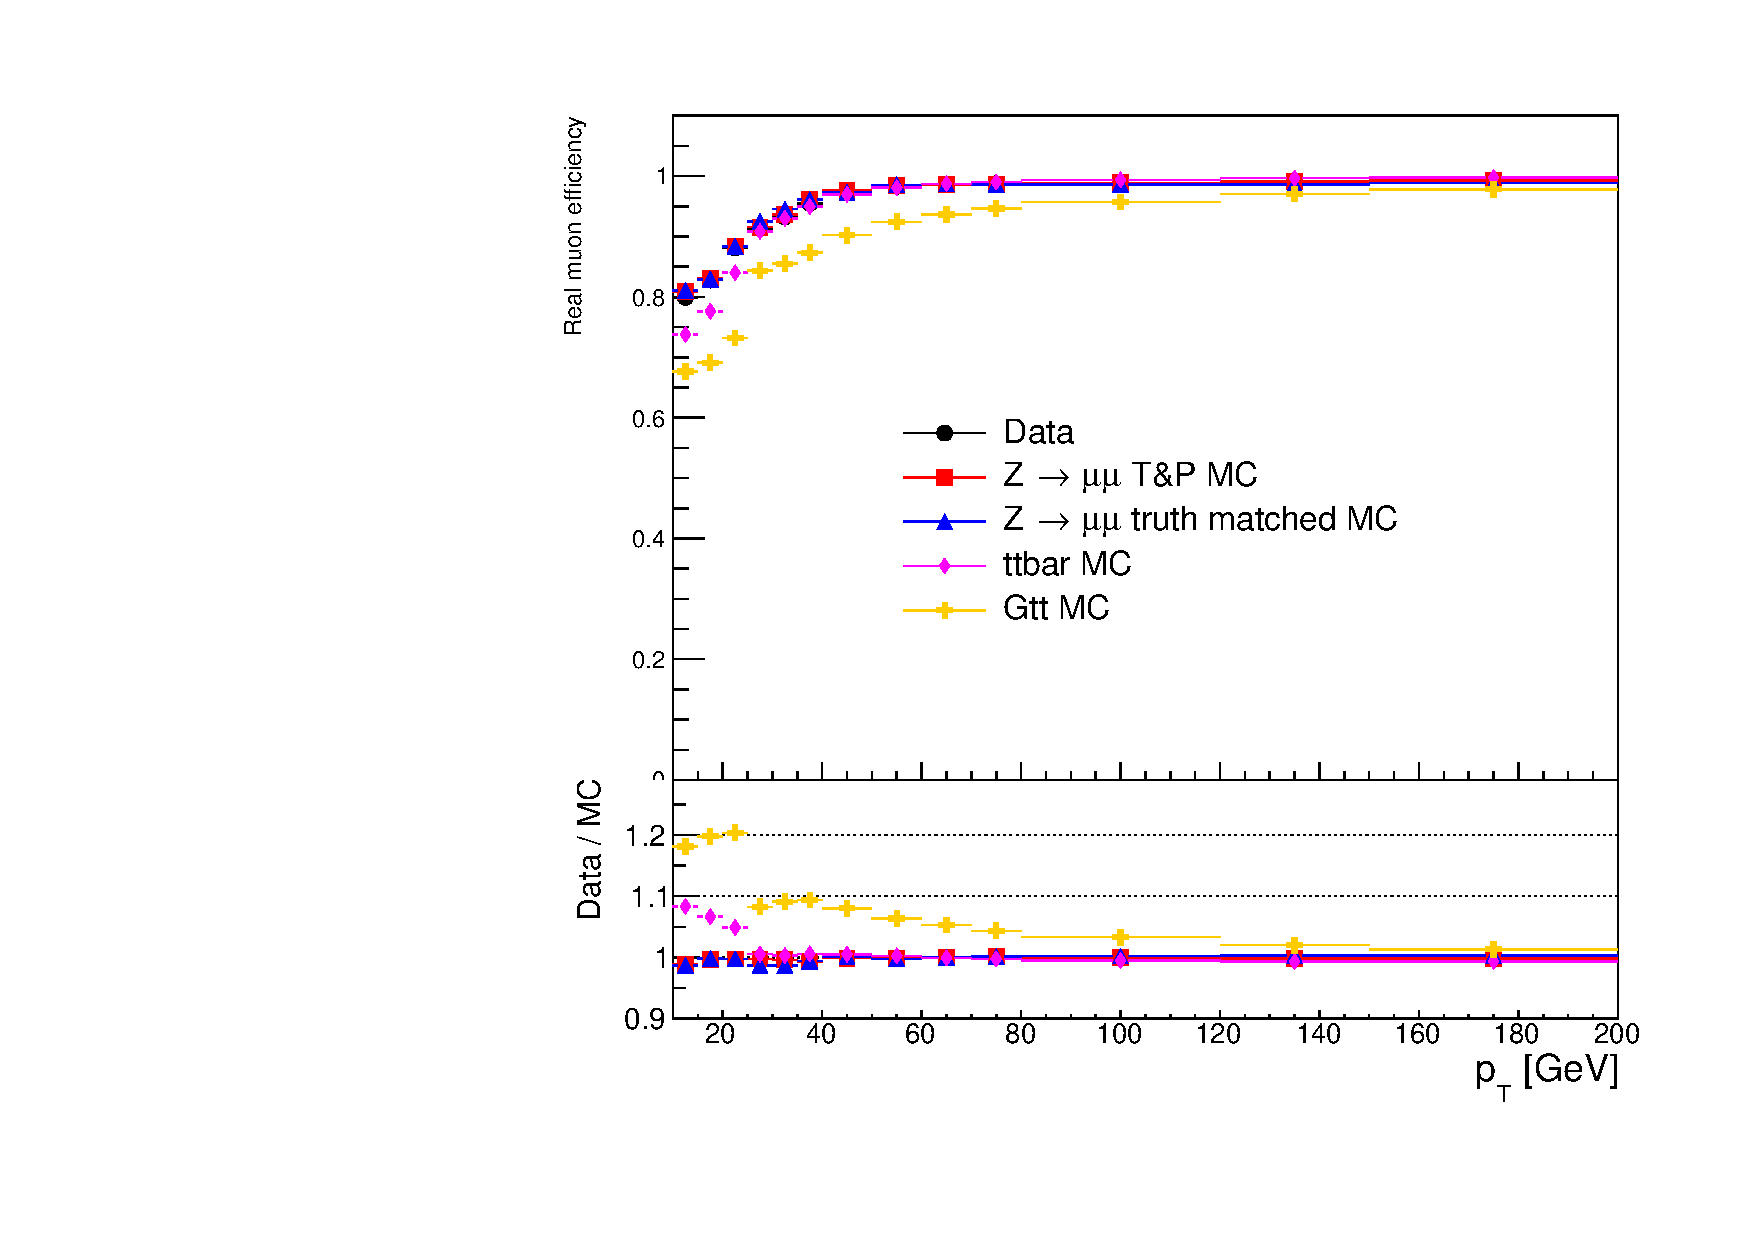
\includegraphics[width=0.48\textwidth]{real_efficiency_ratio_plot_muon_pt_ttbar_gtt.pdf}
\caption{
The electron and muon real efficiencies as a function of $\pt$.
The black dots stands for data, the red squares and blue triangles indicate $Z\to\ell\ell$ tag-and-probe and truth matching, respectively.
The \ttbar and $\tilde{g}\to\ttbar\tilde{\chi^{0}_{1}}$ are represented by magenta diamonds and yellow crosses, respectively.
All of the real lepton efficiencies computed by MC processes are agree with the data one when $\pt>\SI{40}{GeV}$.
The differences in the $\pt<\SI{40}{GeV}$ region come from the different event topologies. 
}
\label{fig:RLE_real_efficiency_ttbar_gtt}
\end{figure}
